%%%%%%%%%%%%%%%%%%%%%%%%%%%%%%%%%%%%%%%%%
% Masters/Doctoral Thesis 
% LaTeX Template
% Version 2.5 (27/8/17)
%
% This template was downloaded from:
% http://www.LaTeXTemplates.com
%
% Version 2.x major modifications by:
% Vel (vel@latextemplates.com)
%
% This template is based on a template by:
% Steve Gunn (http://users.ecs.soton.ac.uk/srg/softwaretools/document/templates/)
% Sunil Patel (http://www.sunilpatel.co.uk/thesis-template/)
%
% Template license:
% CC BY-NC-SA 3.0 (http://creativecommons.org/licenses/by-nc-sa/3.0/)
%
%%%%%%%%%%%%%%%%%%%%%%%%%%%%%%%%%%%%%%%%%


% Plan:
% - Intro
% - Electronic structure
%   - HF
%   - DFT
%   - Excited states
%   - Solid state (PW DFT)
% - Embedding methods
%   - Nothing new
% - Applications
%   - AIE
%   - CI
%   - ESIPT
%   - Excitons
% - JCTC result
% - fromage result
% - Application results
% - Conclusion


%----------------------------------------------------------------------------------------
%	PACKAGES AND OTHER DOCUMENT CONFIGURATIONS
%----------------------------------------------------------------------------------------

\documentclass[
11pt, % The default document font size, options: 10pt, 11pt, 12pt
%oneside, % Two side (alternating margins) for binding by default, uncomment to switch to one side
english, % ngerman for German
singlespacing, % Single line spacing, alternatives: onehalfspacing or doublespacing
%draft, % Uncomment to enable draft mode (no pictures, no links, overfull hboxes indicated)
%nolistspacing, % If the document is onehalfspacing or doublespacing, uncomment this to set spacing in lists to single
%liststotoc, % Uncomment to add the list of figures/tables/etc to the table of contents
%toctotoc, % Uncomment to add the main table of contents to the table of contents
%parskip, % Uncomment to add space between paragraphs
%nohyperref, % Uncomment to not load the hyperref package
headsepline, % Uncomment to get a line under the header
%chapterinoneline, % Uncomment to place the chapter title next to the number on one line
%consistentlayout, % Uncomment to change the layout of the declaration, abstract and acknowledgements pages to match the default layout
]{MastersDoctoralThesis} % The class file specifying the document structure

\usepackage[utf8]{inputenc} % Required for inputting international characters
\usepackage[T1]{fontenc} % Output font encoding for international characters
\usepackage{caption}% single spacing for captions
\captionsetup{font={singlespacing,normalsize}}
\usepackage{mathpazo} % Use the Palatino font by default
\usepackage{braket} % bra ket notation
\usepackage{amsmath}
\usepackage{amsfonts}
\usepackage{amssymb}
\usepackage{bm} %for bold maths
\usepackage{physics}
\usepackage[numbers,super,comma,sort&compress]{natbib}



\usepackage[version=3]{mhchem}
\DeclareUnicodeCharacter{2212}{-}

\usepackage{mathtools}
\usepackage{commath}
\usepackage{siunitx}
%\usepackage[demo]{graphicx}
\usepackage{graphicx}
\usepackage{array,booktabs} %tables
\usepackage{arydshln}
\usepackage{multirow} % multirows in tables
\usepackage{float}%Forces figure placement
\usepackage{siunitx}%Degree symbol
\usepackage{textcomp} % avoids warnings from gensymb
\usepackage{gensymb}
\usepackage{changepage}%center table
\usepackage{caption}
\usepackage{dcolumn}%align in table by decimal
\usepackage{pdfpages}%skill points pdf
\usepackage{hyperref}
\usepackage{verbatim}% comment bloacks
\usepackage{textcomp} %arrow
\usepackage{pifont}% http://ctan.org/pkg/pifont
\usepackage{notoccite}% don't use table of contents to order citations
%\usepackage{imakeidx}% index
\newcommand{\miguel}[1]{\textcolor{black}{#1}}
\newcommand{\mmiguel}[1]{\textcolor{black}{#1}}






%\usepackage[numbers,super,comma,sort]{biblatex} % Use the bibtex backend with the authoryear citation style (which resembles APA)


\usepackage[autostyle=true]{csquotes} % Required to generate language-dependent quotes in the bibliography

%%MACROS

%Embedded cluster
\newcommand{\EC}{OEC}
%Ewald embedded cluster model
\newcommand{\EEC}{OEEC}
%Self consistent Ewald embedded cluster model
\newcommand{\SCEEC}{SC-OEEC}
%2HC1
\newcommand{\HC}{\textbf{HC1}}
%2HC2
\newcommand{\HCC}{\textbf{HC2}}
%HPP
\newcommand{\HPP}{\textbf{HP}}

\DeclareMathOperator\erfc{erfc}

\def\SPSB#1#2{\rlap{\textsuperscript{{#1}}}\SB{#2}}
\def\SP#1{\textsuperscript{{#1}}}
\def\SB#1{\textsubscript{{#1}}}

\newcommand{\cmark}{\ding{51}}%
\newcommand{\xmark}{\ding{55}}%

%----------------------------------------------------------------------------------------
%	MARGIN SETTINGS
%----------------------------------------------------------------------------------------

\geometry{
	paper=a4paper, % Change to letterpaper for US letter
	inner=2.5cm, % Inner margin
	outer=3.8cm, % Outer margin
	bindingoffset=.5cm, % Binding offset
	top=1.5cm, % Top margin
	bottom=1.5cm, % Bottom margin
	%showframe, % Uncomment to show how the type block is set on the page
}

%----------------------------------------------------------------------------------------
%	THESIS INFORMATION
%----------------------------------------------------------------------------------------

\thesistitle{Computational Methods for Photochemistry in Organic Molecular Crystals} % Your thesis title, this is used in the title and abstract, print it elsewhere with \ttitle
\supervisor{Dr. Rachel \textsc{Crespo-Otero}} % Your supervisor's name, this is used in the title page, print it elsewhere with \supname
\examiner{} % Your examiner's name, this is not currently used anywhere in the template, print it elsewhere with \examname
\academicdeg{Doctor of Philosophy} % Your degree name, this is used in the title page and abstract, print it elsewhere with \degreename
\author{Miguel \textsc{Rivera}} % Your name, this is used in the title page and abstract, print it elsewhere with \authorname
\addresses{} % Your address, this is not currently used anywhere in the template, print it elsewhere with \addressname

\subject{Biological Sciences} % Your subject area, this is not currently used anywhere in the template, print it elsewhere with \subjectname
\keywords{} % Keywords for your thesis, this is not currently used anywhere in the template, print it elsewhere with \keywordnames
\university{Queen Mary University of London} % Your university's name and URL, this is used in the title page and abstract, print it elsewhere with \univname
\department{Department of Chemistry} % Your department's name and URL, this is used in the title page and abstract, print it elsewhere with \deptname
\faculty{School of Biological and Chemical Sciences} % Your faculty's name and URL, this is used in the title page and abstract, print it elsewhere with \facname

\AtBeginDocument{
\hypersetup{pdftitle=\ttitle} % Set the PDF's title to your title
\hypersetup{pdfauthor=\authorname} % Set the PDF's author to your name
\hypersetup{pdfkeywords=\keywordnames} % Set the PDF's keywords to your keywords
}

% line spacing
\linespread{1.6}
\begin{document}

\pagestyle{plain} % Default to the plain heading style until the thesis style is called for the body content

%----------------------------------------------------------------------------------------
%	TITLE PAGE
%----------------------------------------------------------------------------------------

\begin{titlepage}
\begin{center}

\vspace*{.06\textheight}
{\scshape\LARGE \univname\par}\vspace{1.5cm} % University name
\textsc{\Large Doctoral Thesis}\\[0.5cm] % Thesis type

\HRule \\[0.4cm] % Horizontal line
{\huge \bfseries \ttitle\par}\vspace{0.4cm} % Thesis title
\HRule \\[1.5cm] % Horizontal line
 
\begin{minipage}[t]{0.4\textwidth}
\begin{flushleft} \large
\emph{Author:}\\
{\authorname} % Author name - remove the \href bracket to remove the link
\end{flushleft}
\end{minipage}
\begin{minipage}[t]{0.4\textwidth}
\begin{flushright} \large
\emph{Supervisor:} \\
{\supname} % Supervisor name - remove the \href bracket to remove the link  
\end{flushright}
\end{minipage}\\[3cm]
 
\vfill

\large \textit{A thesis submitted in fulfilment of the requirements\\ for the degree of \degreename}\\[0.3cm] % University requirement text
\textit{in the}\\[0.4cm]
\deptname\\[2cm] % Research group name and department name
 
\vfill

{\large June 3, 2020}\\[4cm] % Date
%\includegraphics{Logo} % University/department logo - uncomment to place it
 
\vfill
\end{center}
\end{titlepage}

%----------------------------------------------------------------------------------------
%	DECLARATION PAGE
%----------------------------------------------------------------------------------------

\begin{declaration}
\addchaptertocentry{\authorshipname} % Add the declaration to the table of contents
\noindent I, Miguel Rivera, confirm that the research included within this thesis is my own work or that where it has been carried out in collaboration with, or supported by others, that this is duly acknowledged below and my contribution indicated. Previously published material is also acknowledged below.

I attest that I have exercised reasonable care to ensure that the work is original, and does not to the best of my knowledge break any UK law, infringe any third party’s copyright or other Intellectual Property Right, or contain any confidential material.

I accept that the College has the right to use plagiarism detection software to check the electronic version of the thesis.

I confirm that this thesis has not been previously submitted for the award of a degree by this or any other university.

The copyright of this thesis rests with the author and no quotation from it or information derived from it may be published without the prior written consent of the author.

 
\noindent Signed: Miguel Rivera\\
\rule[0.5em]{25em}{0.5pt} % This prints a line for the signature
 
\noindent Date: \today\\
\rule[0.5em]{25em}{0.5pt} % This prints a line to write the date
\end{declaration}

\cleardoublepage

%----------------------------------------------------------------------------------------
%	QUOTATION PAGE
%----------------------------------------------------------------------------------------

\vspace*{0.2\textheight}

\noindent\enquote{\itshape We were working late on the time machine in the little makeshift lab upstairs. The moon was stuck like the whorl of a frozen fingerprint to the skylight. In the back alley, the breaths left behind by yowling toms converged into a fog slinking out along the streets. Try as we might, our measurements were repeatedly off. In one direction, we'd reached the border at which clairvoyants stand gazing into the future, and in the other we'd gone backward to the zone where the present turns ghostly with memory and yet resists quite becoming the past. We'd been advancing and retreating by smaller and smaller degrees until it had come to seem as if we were measuring the immeasurable. Of course, what we really needed was some new vocabulary of measurement. It was time for a break.}\bigbreak

\hfill Stuart Dybek, \textit{Paper Lantern}

%----------------------------------------------------------------------------------------
%	ABSTRACT PAGE
%----------------------------------------------------------------------------------------

\begin{abstract}
\addchaptertocentry{\abstractname} % Add the abstract to the table of contents
\setstretch{1.1}
Organic molecular crystals hold great promise for photochemical applications such as photovoltaics, OLEDs or lasers. Understanding the excited states of these systems is particularly challenging due to the interconnectedness of the excited state character of the molecular wavefunctions and the environmental interactions within the condensed phase. The principal obstacle to this understanding is first and foremost the methodological gap between periodic simulation methods and molecular scale excited state formalisms. Multiscale cluster model methods are a viable extension of the latter, where they promise to recover the crystalline environmental interactions for excited state calculations whilst representing excitations as localised defects rather than periodic delocalised perturbations. This is pertinent to molecular crystals\textemdash{}periodic but non-covalently bonded, displaying quasilocal excitations\textemdash{}however, there is hitherto no software package dedicated their modelling as clusters.

The principal output of this project is the development and application of such a program. This thesis begins with a review of the theoretical background necessary to understand QM:QM' (Quantum Mechanics:Quantum Mechanics') cluster models for excited states, namely quantum electronic structure modelling methods, multiscale embedding methods, and molecular photochemistry. Then, three results chapters are presented, each based on a publication carried out during the project. First, the cluster model method is described, where the electrostatic embedding of the QM region has been extended to model the Madelung potential. Then, the program (\texttt{fromage}, the FRamewOrk for Molecular AGgregate Excitations) which implements this method is presented, along with a suite of analysis tools and command line utilities which enable the reproducible investigation of cluster geometries in molecular crystals. Finally, \texttt{fromage} is used to model an array of luminescent materials and investigate their competing radiative and nonradiative excited state decay pathways.
\end{abstract}

%----------------------------------------------------------------------------------------
%	ACKNOWLEDGEMENTS
%----------------------------------------------------------------------------------------

\begin{acknowledgements}
\addchaptertocentry{\acknowledgementname} % Add the acknowledgements to the table of contents
This thesis summarises the work that I carried out between October 2016 and March 2020. Whilst it did cost an undeniably large amount of effort, CPU hours, and keystrokes, it was overall a pleasure and privilege, thanks to the support of a group of outstanding entities which I will proceed to list.

I give my thanks to the members of my panel at QMUL. Isaac Abrahams, for chairing meetings and Devis Di Tommaso for being my second supervisor, always supportive and available to talk about science or careers.

All of the workers of the Joseph Priestley building deserve a mention, for solidarity and good mood. Thank you for Friday drinks at the Senior Common Room on a Friday evening, coffee while waiting for a fire alarm to blow over, or miming conversations through the plexiglass that separates the wet lab and computational office.

Speaking of the latter, the Computational Chemists at QMUL were my closest colleagues for these past years, and I am grateful to all of them for their support. To Anna, Bob, Dimitri, Etienne, Fariha, Filip, Fu, Matteo, and Xiangwen thank you for conversations, lunches, teas, and compassion.

Now I reach the point of my research group, where individual mentions are in order. Scott and Warda stand out as a duo of pre-PhD students who exceeded every expectation but became friends and colleagues, despite my ruining their learning by trying to explain k-space to them. Sorry about that. Ljiljana has been a supportive and compassionate presence ever since she arrived in the UK, and will receive my unreserved thanks just as soon as she watches and returns my DVD of \textit{Ast\'erix et Obélix : Mission Cl\'eop\^atre}. Federico is only a recent addition, but has already proven himself a great deskmate, and a power user of \texttt{fromage}, for which I can only admire his taste. Amir has been an incredibly hard working and fast learning PhD-mate, and it has been a privilege to share some of my new expertise with him. Michael, thank you for providing an example of how to manage science and Rachel, and how to care only the right amount. Your bash-fu is unmatched amongst peers, as can only be evidenced by your program “cdjob”, which literally must have saved me about a day of my life so far in typing. Back of the net!

I would also like to thank the Thomas Young Centre organisers and community, for making me feel a part of a larger group of researchers, and allowing me to share hardships with so many peers. To Bethan, Matthias, Patrick, Sam, and many others, I would like to present my gratitude.

Here seems as good a point as any to thank the communities which made my technical life easy and rewarding during my PhD. The list of useful programs and forums is extensive, so I will only highlight my favourites: vim, Stack Overflow, vmd, Chemcraft, Jmol, Psi4, GNU/Linux, \LaTeX{}, and the Python project.

Now for the extracurricular acknowledgments. I would like to extend my gratitude to my flatmates with whom I shared three-odd years in the Bethnal Green apartment; Dag, Devi, Jolien, and Merry (Emma, Lachlan and Yean get honorable mentions here). Your kindness and caring are only matched by the amount of disassembled mannequin parts scattered around your lair. More specifically, thank you: Dag for warmth, Devi for attentiveness, Jolien for care, and Merry for joy. Let the record show that the final stretch of this thesis is being written on Merry’s antique laptop, which was delivered to me by Yean.

To my comrades in board games, roleplaying games, card games, and any other kind of games, thank you for late nights, laughs, camaraderie, and victories. Of those not yet mentioned, I add Dan, Emrys, Emy, Feargus, Hugo, Jasper, Oli, Ryan, and Sally.

Members of my musical sphere also deserve my gratitude, and I would like to thank for grooves, hummings, and wailings: Ben, Charlie, Harry, Jamie, Max, Mike, The Roundhouse Choir, and The Martinis.

Arthur and Matt must be singled out for being a part of all of the above adventures, and more. Thank you for everything. You know what you did.

I would like to thank Kasia, for her support and presence during some of the hardest parts of this story, as well as all of the other wonderful human beings that she allowed me to meet in Poland and elsewhere.

This thesis is written with calm and joy, thanks in no small part to Lucie, and her innate glow. You are wonderful, caring, and really good at eating apples. Thank you also, and by extension, to the members of the Hiron clan, for their giddiness and blissful chaos. The Grafton Road Noodles, also deserve my warmest thanks, for my countless invasions. Marty, for cool moves, Jay for delight, and \'Elise for peace and for taking Lucie to a Brad Mehldau Concert in March 2019.

To my family in France, Switzerland, Colombia, Canada, Spain, London, and any other number of satellite countries, my absolute thanks. You are a well of warmth, kindness, and practicality, which has served me my whole life, but particularly in the last four years. Thank you to my parents for support, homegrown vegetables, and bash advice, and to my brother Alejandro, for dedication, conversations, and altruism.

There only remains to thank the true mastermind behind this thesis, Rachel. I don’t think I have ever told you this, but when I am asked what my supervisor is like, I usually compare you to Yoda. You are cheerful and aloof, which fools unsuspecting Jedi into underestimating your vastly superior Force power (here, the Force, is excited state Computational Chemistry). With the hindsight of a few years, I can safely assert what I started to suspect only a few months after meeting you: when we disagree, you are usually right, and it’s better to just follow your advice in the first place before opposing any sort of battle (you can show this sentence to future PhD students, just try to hide your smugness). I chose to pursue this project in great part because of your and Michael’s characters, and you have proven that it was one of the best decisions of my life. Your combination of patience, joy, and rigour have brought me comfort and guidance at the worst lows of the project (e.g. after having to repeat months’ worth of calculations because of a typo, or when my personal life got in the way). You have granted me confidence, expertise, and wisdom, and allowed me to preserve my life alongside an ambitious work project. For your support, presence, music recommendations, and pad thais at the Rusty Bike thank you. Anita and David are in good company.

This acknowledgments page is being written at a time of global crisis. In the spirit of camaraderie, and whatever the situation of the reader, I would like to extend my sincere sympathies for the hardships they may be encountering, however large or small, and solidarity in the obstacles to come.

\end{acknowledgements}

%----------------------------------------------------------------------------------------
%	LIST OF CONTENTS/FIGURES/TABLES PAGES
%----------------------------------------------------------------------------------------

\tableofcontents % Prints the main table of contents

\listoffigures % Prints the list of figures

\listoftables % Prints the list of tables

%----------------------------------------------------------------------------------------
%	ABBREVIATIONS
%----------------------------------------------------------------------------------------

\begin{abbreviations}{ll} % Include a list of abbreviations (a table of two columns)

\textbf{ADC2} & \textbf{A}lgebraic \textbf{D}iagrammatic \textbf{C}onstruction \textbf{2}\\
\textbf{AIE} & \textbf{A}ggregation \textbf{I}nduced \textbf{E}mission\\
\textbf{BO} & \textbf{B}orn-\textbf{O}ppenheimer\\
\textbf{CASPT2} & \textbf{C}omplete \textbf{A}ctive \textbf{S}pace \textbf{P}erturbation \textbf{T}heory \textbf{2}\\
\textbf{CASSCF} & \textbf{C}omplete \textbf{A}ctive \textbf{S}pace \textbf{S}elf-\textbf{C}onsistent \textbf{F}ield\\
\textbf{CC} & \textbf{C}oupled \textbf{C}luster\\
\textbf{CCS} & \textbf{C}oupled \textbf{C}luster \textbf{S}ingles\\
\textbf{CCSD} & \textbf{C}oupled \textbf{C}luster \textbf{S}ingles and \textbf{D}oubles\\
\textbf{CGF} & \textbf{C}ontracted \textbf{G}aussian \textbf{F}unction\\
\textbf{CI} & \textbf{C}onfiguration \textbf{I}nteraction\\
\textbf{CSF} & \textbf{C}onfiguration \textbf{S}tate \textbf{F}unction\\
\textbf{CT} & \textbf{C}harge \textbf{T}ransfer\\
\textbf{DFT} & \textbf{D}ensity \textbf{F}unctional \textbf{T}heory\\
\textbf{DFTB} & \textbf{D}ensity \textbf{F}unctional \textbf{T}ight-\textbf{B}inding\\
\textbf{FC} & \textbf{F}rank-\textbf{C}ondon\\
\textbf{FGR} & \textbf{F}ermi’s \textbf{G}olden \textbf{R}ule\\
\textbf{fromage} & \textbf{FR}amew\textbf{O}rk for \textbf{M}olecular \textbf{AG}gregate \textbf{E}xcitations\\
\textbf{GGA} & \textbf{G}eneralised \textbf{G}radient \textbf{A}pproximation\\
\textbf{GTO} & \textbf{G}aussian \textbf{T}ype \textbf{O}rbital\\
\textbf{HF} & \textbf{H}artree-\textbf{F}ock\\
\textbf{IMOMM} & \textbf{I}ntegrated \textbf{M}olecular \textbf{O}rbital \textbf{M}olecular \textbf{M}echanics\\
\textbf{IMOMO} & \textbf{I}ntegrated \textbf{M}olecular \textbf{O}rbital \textbf{M}olecular \textbf{O}rbital\\
\textbf{KS} & \textbf{K}ohn-\textbf{S}ham\\
\textbf{LDA} & \textbf{L}ocal \textbf{D}ensity \textbf{A}pproximation\\
\textbf{MM} & \textbf{M}olecular \textbf{M}echanics\\
\textbf{MP2} & \textbf{M}{\o}ller \textbf{P}lesset \textbf{2}\\
\textbf{MRCI} & \textbf{M}ultireference \textbf{C}onfiguration \textbf{I}nteraction\\
\textbf{MRSCF} & \textbf{M}ultireference \textbf{S}elf-\textbf{C}onsistent \textbf{F}ield\\
\textbf{OLED} & \textbf{O}rganic \textbf{L}ight \textbf{E}mitting \textbf{D}iode\\
\textbf{ONIOM} & \textbf{O}wn \textbf{N}-layered \textbf{I}ntegrated molecular \textbf{O}rbital\\& and molecular \textbf{M}echanics for \textbf{Q}uantum \textbf{M}echanics\\
\textbf{PBE} & \textbf{P}erdew-\textbf{B}ecke-\textbf{E}rnzerhof\\
\textbf{PCM} & \textbf{P}olarisable \textbf{C}ontinuum \textbf{M}odel\\
\textbf{QE} & \textbf{Q}uantum \textbf{E}fficiency\\
\textbf{QM} & \textbf{Q}uantum \textbf{M}echanics\\
\textbf{RACI} & \textbf{R}estricted \textbf{A}ccess to \textbf{C}onical \textbf{I}ntersections\\
\textbf{RIM} & \textbf{R}estriction of \textbf{I}ntramolecular \textbf{M}otions\\
\textbf{SCF} & \textbf{S}elf-\textbf{C}onsistent \textbf{F}ield\\
\textbf{SE} & \textbf{S}hr\"{o}dinger \textbf{E}quation\\
\textbf{SLE} & \textbf{S}olid state \textbf{L}uminescent \textbf{E}nhancement\\
\textbf{TDDFT} & \textbf{T}ime-\textbf{D}ependent \textbf{D}ensity \textbf{F}unctional \textbf{T}heory\\
\textbf{TISE} & \textbf{T}ime \textbf{I}ndependent \textbf{S}hr\"{o}dinger \textbf{E}quation\\
\end{abbreviations}

%----------------------------------------------------------------------------------------
%	THESIS CONTENT - CHAPTERS
%----------------------------------------------------------------------------------------

\pagestyle{thesis} % Return the page headers back to the "thesis" style

% Include the chapters of the thesis as separate files from the Chapters folder
% Uncomment the lines as you write the chapters

% Chapter 1
\chapter*{Introduction}% Main chapter title
\addcontentsline{toc}{chapter}{Introduction}  
\label{Chapter1} % For referencing the chapter elsewhere, use \ref{Chapter1} 

%----------------------------------------------------------------------------------------

% Define some commands to keep the formatting separated from the content 
\newcommand{\keyword}[1]{\textbf{#1}}
\newcommand{\tabhead}[1]{\textbf{#1}}
\newcommand{\code}[1]{\texttt{#1}}
\newcommand{\file}[1]{\texttt{\bfseries#1}}
\newcommand{\option}[1]{\texttt{\itshape#1}}

%----------------------------------------------------------------------------------------

The luminescent response of molecular crystals has found applications in several recent and impactful technologies such as biosensing devices, Organic Light Emitting Diodes (OLEDs), field-effect-transistors, lasers, and photovoltaics.\cite{Li2012,Kwok2015,Huang2013,Zhao2011,Aldred2013,Gierschner2016,Hains2010,Lee2015} However, the theoretical investigation of the photochemistry of solids has not been as reliable an experimental aid as that of liquids or gases, due to the added complexity associated with modelling condensed phases. Indeed the calculation of a molecular excited states is often restricted to the low hundreds of atoms due to its prohibitive computational cost and theoretical inadequacy for extended correlated systems. On the other hand, solids are often defined by their long-range interactions, which can involve moles of collaborating atoms for periodic systems. Molecular condensed phases held together by van der Waals forces occupy a liminal space in this picture, where due to their non-bonded nature, they share properties both of crystals and single molecules, indicating that an overlap in methodologies could be used to investigate their excited states in a robust way.

In recent years, multiscale modelling methods such as "our Own N-layered Integrated molecular Orbital and molecular Mechanics for Quantum Mechanics:Quantum Mechanics'" (ONIOM QM:QM')\cite{Humbel1996,Svensson1996} have proven a useful asset in modelling the excited states of molecular crystals.\cite{Kochman2013,Kochman2013a,Presti2014,Presti2016,Presti2016a,Presti2017,Wilbraham2016a} Cluster model methods represent excitations as defect perturbations rather than fully delocalised phenomena as in full unit-cell periodic excited state calculations. They also limit the amount of molecules to be calculated in the excited state in all cases but the ones with smallest unit cells. Finally, their use of local orbital basis sets avoids the increased computational cost of plane-wave Density Functional Theory (DFT) for highly accurate functionals, which remains a topic of research.\cite{Bowler2012} Hybrid DFT and post-Hartree-Fock methods are therefore available within the cluster model paradigm.

However the conventional ONIOM QM:QM' method presents several weaknesses in modelling the condensed phase:
\begin{enumerate}
    \item The system-environment interactions between the excitation and the crystal are truncated to include only the nearest neighbours.
    \item The electrostatic interactions are modelled as point charge potentials whose charge values are not uniquely defined.
    \item The response of the environment to the electronic reorganisation of the system is ignored.
    \item They lack an implementation tailored to excited organic molecular crystals.
\end{enumerate}
These shortcomings are elaborated upon in Section \ref{sec:problems}, after presenting the necessary theoretical framework to understand them.

\textbf{The object of this thesis is to offer solutions to the above problems in QM:QM' modelling for excited states in organic molecular crystals, in the form of new modelling methods implemented in a software package, and to apply these methods in order to understand luminescent phenomena in systems previously difficult to model.}

A principal outcome of the doctoral project, along with the publications cited throughout and this thesis, is the program \texttt{fromage}, the FRamewOrk for Molecular AGgregate Excitations. Readers interested in the practical applications of the topics discussed herein can peruse the software project at: \href{https://github.com/Crespo-Otero-group/fromage}{https://github.com/Crespo-Otero-group/fromage}.

The present work is split in two parts. Part I focuses on the required theoretical background to understand the use of cluster models to model photochemistry in molecular crystals. Chapter 1 introduces the quantum mechanical modelling methods which are used throughout, Chapter 2 presents the embedding schemes employed to allow these methods to account for a system's environment, and Chapter 3 introduces foundational topics in photochemistry which will help contextualise what it is that the cluster models are to simulate. Then, Part II presents the results of the thesis. Chapter 4 introduces new ONIOM QM:QM' cluster models tailored to model excited molecular crystals, Chapter 5 describes the program which implements them and other auxiliary tools for analysing these systems, and Chapter 6 investigates of the competing radiative and nonradiative mechanisms of an array of luminescent organic crystals, relying on the new methodological advances.

The following publications constitute the broader output of this doctorate:
\begin{itemize}
\linepenalty100
    \item M. Dommett, M. Rivera and R. Crespo-Otero, How Inter- and Intramolecular Processes Dictate Aggregation-Induced Emission in Crystals Undergoing Excited-State Proton Transfer. \textit{J. Phys. Chem. Lett.}, 2017, \textbf{8} (24), 6148–6153.
    \item M. Rivera, M. Dommett and R. Crespo-Otero, ONIOM(QM:QM') Electrostatic Embedding Schemes for Photochemistry in Molecular Crystals. \textit{J. Chem. Theory Comput.}, 2019, \textbf{15} (4), 2504–2516. \hbox{}\hfill \textbf{Chapter \ref{chap:jctc}}
    \item M. Dommett, M. Rivera, M. T. H. Smith and R. Crespo-Otero, Molecular and Crystalline Requirements for Solid State Fluorescence Exploiting Excited State Intramolecular Proton Transfer. \textit{J. Mater. Chem. C}, 2020, \textbf{8} (7), 2558–2568.
    \item M. Rivera, M. Dommett, A. Sidat, W. Rahim and R. Crespo‐Otero, fromage : A Library for the Study of Molecular Crystal Excited States at the Aggregate Scale. \textit{J. Comput. Chem.}, 2020, \textbf{41} (10), 1045–1058. \hfill \textbf{Chapter \ref{chap:prog}}
    \item M. Rivera, L. Stojanovi\'c, R. Crespo-Otero, Competition between radiative and nonradiative excited state processes in photoluminescent organic molecular crystals. \textit{in preparation}, 2020. \hfill \textbf{Chapter \ref{chap:molecules}}
    \item V. Posilgua, D. Pandya, M. Rivera, R. Crespo-Otero, R. Grau-Crespo, Two-dimensional porphyrin-based metal organic frameworks for photocatalytic water splitting: a computational investigation. \textit{in preparation}, 2020.
\end{itemize}



\part{Background}
\chapter{Electronic Structure Methods} % Main chapter title

\label{chap:meth}

NB: The notation in this chapter is largely borrowed from the following texts: \textit{Modern Quantum Chemistry: Introduction to Advanced Electronic Structure Theory} by Szabo and Ostlund,\cite{Szabo} \textit{Time-Dependent Density-Functional Theory: Concepts and Applications} by Ullrich,\cite{Ullrich} and \textit{Quantum Theory of the Solid State: An Introduction} by Kantorovich.\cite{Kantorovich2004}


\section{Wavefunctions Methods}

The state function of a nonrelativistic quantum mechanical system is wholly described by the Shr\"{o}dinger equation (SE):
\begin{equation}
    i\hbar \frac{d}{dt} \ket{\Psi(t)} = \hat{H} \ket{\Psi(t)}
    \label{eq:tdse}
\end{equation}
Where the $\ket{\Psi(t)}$ is the time dependent wave function, and $\hat{H}$ is the Hamiltonian operator. In a system of $N$ electrons and $M$ nuclei, $\hat{H}$ has the form:

\begin{equation}
    \hat{H} = - \sum_{i=1}^N \frac{1}{2} \nabla^2_i
              - \sum_{A=1}^M \frac{1}{2M_A} \nabla^2_A
              - \sum_{i=1}^N \sum_{A=1}^M \frac{Z_A}{r_{iA}}
              + \sum_{i=1}^N \sum_{j>i}^N \frac{1}{r_{ij}}
              + \sum_{A=1}^M \sum_{B>A}^M \frac{Z_AZ_B}{r_{AB}}
    \label{eq:full_hamilton}
\end{equation}

Where $\nabla^2_i$ and $\nabla^2_A$ are the Laplacian operators acting on electrons and nuclei respectively, $Z_A$ is the charge of nucleus $A$ and $r_{AB}$ is the distance between points $A$ and $B$.

In an equilibrium, the quantum system becomes time independent by definition, and has a simpler equation of state, the  time-independent Shr\"{o}dinger equation (TISE):\cite{Schrodinger1926}
\begin{equation}
    \hat{H} \ket{\Psi} =  E \ket{\Psi}
    \label{eq:tise}
\end{equation}
Where $\ket{\Psi}$ is the time independent wave function and $E$ its associated energy.

\subsection{The Born-Oppenheimer Approximation}

The SE is analytically unsolvable for any system with more than two particles. We must therefore employ approximations to model chemically meaningful situations.

Nuclei are several orders of magnitude heavier than electrons, suggesting that the Hamiltonian can be split into an electronic and a nuclear term. The electronic term treats nuclei as static potentials, and can yield an electronic wavefunction, uncorrelated with the nuclear one, which does not take into account the nuclear kinetic and internuclear potential terms of Equation \ref{eq:full_hamilton}:

\begin{equation}
    \hat{H}_{el} = - \sum_{i=1}^N \frac{1}{2} \nabla^2_i
              - \sum_{i=1}^N \sum_{A=1}^M \frac{Z_A}{r_{iA}}
              + \sum_{i=1}^N \sum_{j>i}^N \frac{1}{r_{ij}}
    \label{eq:el_ham}
\end{equation}

\begin{equation}
    \hat{H}_{el} \Phi = E_{el} \Phi
    \label{eq:el_tise}
\end{equation}

This is known as the Born-Oppenheimer (BO) approximation, and allows for the nuclear coordinates to be considered only parametrically when calculating the energy of a given nuclear geometry.\cite{Born1927}

\subsection{Many-Electron Wavefunctions}

Electrons are fermions of spin 1/2. Therefore the wavefunction which describes an electron should contain both a spatial part ($\psi(\bm{r})$), and a spin part ($\alpha(\omega)$ or $\beta(\omega)$ for spin up or down). Single electron wavefunctions are therefore called spin orbitals and, for example for spin up, are written:
\begin{equation}
\begin{split}
    \chi(\bm{x}) &= \psi(\bm{r})\alpha(\omega)\\
    \ket{\chi} &= \ket{\psi}\ket{\alpha}
    \label{eq:spinorb}
\end{split}
\end{equation}
Where the $\bm{x}$ coordinate contains both the position $\bm{r}$ and the spin $\omega$.

A many electron wavefunction should be constructed taking into account the properties of fermions that they are antisymmetric under exchange. To fulfil $\Psi(\bm{x_1},\bm{x_2}) = - \Psi(\bm{x_2},\bm{x_1})$, we can exploit the property of the matrix determinant, which changes sign with the interchange of row or column. This kind of wavefunction is called the Slater determinant:\cite{Slater1929}

\begin{gather}
    \Psi^{SD}(\bm{x_1},\bm{x_2},\ldots,\bm{x_N}) 
    = (N!)^{-1/2}
      \begin{vmatrix}
   \chi_i(\bm{x}_1) & \chi_j(\bm{x}_1) & \dotsm & \chi_k(\bm{x}_1) \\
   \chi_i(\bm{x}_2) & \chi_j(\bm{x}_2) & \dotsm & \chi_k(\bm{x}_2) \\
   \vdots           & \vdots           &        & \vdots           \\
   \chi_i(\bm{x}_N) & \chi_j(\bm{x}_N) & \dotsm & \chi_k(\bm{x}_N) 
   \end{vmatrix}
\end{gather}

In Dirac notation, we adopt the convention $\Psi^{SD}(\bm{x_1},\bm{x_2},\ldots,\bm{x_N}) = \ket{\bm{x_1}\bm{x_2}\ldots\bm{x_N}}$.


\subsection{The Hartree-Fock Method}
We now wish to find a method to compute all spin orbitals of the electronic system's Slater determinant to obtain the most accurate wavefunction possible. To do so, for each spin orbital, we write a one-electron secular equation:
\begin{equation}
    f(1)\chi(\bm{x}_1) = \epsilon  \chi(\bm{x}_1)
    \label{eq:one_electron_HF}
\end{equation}
    
$f(1)$ is called the Fock operator, and is written:

\begin{equation}
    f(1) = h(1) + v^{HF}(1)
\end{equation}{}

Where $h(1)$ is the one-electron core Hamiltonian:

\begin{equation}
    h(1) = - \frac{1}{2} \nabla^2_1 - \sum_{A=1}^M \frac{Z_A}{r_{1A}}
\end{equation}{}

And $v^{HF}(1)$ is the Hartree-Fock (HF) potential, associated with the multi-electronic interaction energy. It, in turn, is comprised of Coulomb and exchange electron-electron interactions, and is expressed:
\begin{equation}
    v^{HF}(1)=\sum_{b}(\mathcal{J}_b(1) - \mathcal{K}_b(1))
\end{equation}

Where the Coulomb operator $\mathcal{J}_b(1)$ expresses the electrostatic potential on the electron $1$ in orbital $\chi_a$ from electron $2$ in orbital $\chi_b$:
\begin{equation}
    \mathcal{J}_b(1) = \int \frac{|\chi_b(2)|^2}{r_{12}} d\bm{x}_2
\end{equation}
The exchange operator, on the other hand, is a nonlocal operator; it depends on the value of $\chi_a$ at points of space different from $\bm{x}_1$ as follows:
\begin{equation}
    \mathcal{K}_b(1)\chi_a(1) = \left[\int \chi_b(2)^*r^{-1}_{ij}\chi_a(2) d\bm{x}_2\right]\chi_b(1)
\end{equation}

In its full form, the Fock operator is therefore:\cite{Hartree1935,Fock1930,Fock1930a}

\begin{equation}
    f(1) = - \frac{1}{2} \nabla^2_1 - \sum_{A=1}^M \frac{Z_A}{r_{1A}} + \sum_{b} (\mathcal{J}_b(1) - \mathcal{K}_b(1))
\end{equation}

% In a closed shell system of $N$ electrons, the spatial Fock operator can be shown to adopt the form:
% \begin{equation}
%     f(1) = h(1) + \sum_a^{N/2} 2J_a(1)-K_a(1)
% \end{equation}
% where the closed-shell Coulomb and exchange operators are:
% \begin{equation}
%     \begin{split}
%         &J_a(1)=\int\psi^*_a(2)r^{-1}_{12}\psi_a(2)\\
%         &K_a(1)\psi_i(1) = \left[\int  \psi^*_a(2)r^{-1}_{12} \psi_a(1) d\bm{r}_2  \right] \psi_a(1)
%     \end{split}
% \end{equation}

\subsection{Atomic Orbital Basis Sets}
The two above operators involve the integration of products of spatial orbitals. If we could decompose these orbitals in an infinite number of functions spanning all of space, this would yield an exact spin orbital within the constraints of Hartree-Fock theory. However, due to the computational constraints of our finite central processing units, we must settle for an easily integrable set of functions which are arranged in a physically meaningful way. 

In the context of a molecular system, it makes most sense to employ sets of atom-centred functions which have the shapes of individual electrons about a particular nucleus. These are called atomic orbitals, and their linear combination makes up a molecular orbital. If our set has $K$ basis functions, we write spatial orbital $\psi_i$:

\begin{equation}
    \psi_{i} = \sum_{\mu = i}^K C_{\mu i}\phi_{\mu}
    \label{eq:lcao}
\end{equation}

For ease of integration, we often use a solutions of the hydrogen atom multiplied by Gaussian radial component. This is called a Gaussian Type Orbital (GTO). However, the behaviour of Gaussian functions in the limit of large distance does not necessarily reflect the behaviour of atomic orbitals, which instead follow an inverse law, thus in practice we use linear combinations of several GTOs, whose coefficients are called contractions, explaining the name Contracted Gaussian Functions (CGFs).

Oftentimes, the valence electrons are assigned more than one CGF, to obtain a better resolution of the interatomic interactions. Basis sets with several CGFs per valence electron are called split valence, or Pople basis sets if they are written in the form \textit{X-YZG}. For example, the basis set 6-31G has six GTOs per core electron basis function, and two CFGs for valence electrons, one with three GTOs and one with one GTO.

Additionally, the basis sets may be complemented by diffuse Gaussians to accurately describe the region of the atom far from the nucleus, or asymmetric functions to represent the polarisability of the atom. A 6-31G basis set complemented by diffuse and polarisable functions is written 6-31G(d,p).

\subsection{The Roothaan Equations}

Armed with our basis set, we are able to re-write the HF equation in matrix form by enclosing the Fock operator with basis functions. We write:

\begin{equation}
    \bm{F} \bm{C} = \bm{S} \bm{C} \bm{\epsilon}    
\label{eq:rooth}
\end{equation}

Where the Fock matrix has elements $F_{\mu \nu} = \int \phi^*_{\mu}(1)f(1)\phi_{\nu}(1)d\bm{r}_1$, $\bm{S}$ is the overlap matrix with elements $S_{\mu \nu} = \int \phi_{\mu}^*(1) \phi_{\nu}(1) d\bm{r}_1$, which account for the nonorthogonality of the basis, $\bm{C}$ defines the basis coefficients of the spin orbitals in Equation \ref{eq:lcao}, and $\bm{\epsilon}$ is the diagonal matrix of orbital energies:

\begin{gather}
    \bm{\epsilon} =
  \begin{pmatrix}
    \epsilon_{1} & & \mbox{\Large 0}\\
    & \ddots & \\
    \mbox{\Large 0} & & \epsilon_K
  \end{pmatrix}
\end{gather}

 The equations originating from the canonical Equation \ref{eq:rooth} are called the Roothaan equations. They can be manipulated to become orthogonal, and adopt a solvable form without the interfering overlap matrix. A particularity of the Roothaan equations is that since the Fock matrix contains the HF potential, it depends on the spin orbitals, which are themselves defined in $\bm{C}$. This indicates that the Roothaan equations must be solved iteratively, in order to find a self-consistent set of spin-orbitals. This procedure is known as the Self-Consistent Field (SCF) method.

The SCF method allows us to obtain a set of $K$ spatial orbitals and thus $2K$ spin orbitals. If we construct a wavefunction which is the Slater determinant of the $N$ lowest spin orbitals, we obtain the HF ground state:
\begin{equation}
    \ket{\Psi_0} = \ket{\chi_1 \chi_2 \ldots \chi_K}
\end{equation}

\subsection{Electronic Correlation}

The $N$ spin orbitals which make up the HF ground state are called \textit{occupied} orbitals, while all of the higher energy spin orbitals are \textit{virtual} orbitals.

We can construct new Slater determinants by swapping out occupied orbitals for virtual orbitals from the HF ground state. These are called excited Slater determinants, and are characterised by the amount of virtual orbitals included at one time, for instance, single excitation, double excitation and so on. The real wavefunction has the conformational space to adopt any combination of excited determinants, therefore, ignoring the size of the basis set, the best possible description of the nonrelativistic BO wavefunction would be a linear combination of all HF Slater determinants.

\begin{equation}
    \ket{\Phi} = c_0 \ket{\Psi_0} + \sum_{ra} c^r_a\ket{\Psi^r_a} + \sum_{\substack{a<b\\r<s}} c^{rs}_{ab}\ket{\Psi^{rs}_{ab}} + \sum_{\substack{a<b<c\\r<s<t}} c^{rst}_{abc}\ket{\Psi^{rst}_{abc}} + \ldots
    \label{eq:fullci}
\end{equation}

Where $\ket{\Psi_{\{\alpha\beta\ldots\}}^{\{\mu\nu\ldots\}}}$ is the Slater determinant with the excitations $\alpha\rightarrow\mu, \beta\rightarrow\nu \ldots$ with the corresponding expansion coefficient $c_{\{\alpha\beta\ldots\}}^{\{\mu\nu\ldots\}}$. $\ket{\Phi}$ is called the full configuration interaction (CI) wavefunction.

Due to the explosively increasing number of terms of the full CI wavefunction, it is impractical to calculate for systems of more than a few electrons. However, it gives us a formal definition for the error in the HF ground state. We define the \textit{correlation} energy as the difference between the energies of the HF ground state ($E_0$) and full CI wavefunctions ($\mathcal{E}_0$):

\begin{equation}
    E_{\text{corr}} = \mathcal{E}_0 - E_0
\end{equation}

Several methods have been developed to recover correlation energy by including the effect of excited determinants in the HF ground state.

\subsection{M{\o}ller Plesset Perturbation Theory}
Rayleigh–Schr{\"o}dinger perturbation theory is a numerical method in quantum mechanics which corrects small errors in approximate wavefunctions in the form of an asymptotic series. If we use the Fock operator, shifted by the sum of the orbital energies, as the the reference wavefunction, then the correlation energy can act as the perturbation.\cite{Moller1934}

The order of the asymptotic series increases with cost and accuracy of the method. At first order, this energy\textemdash{}called M{\o}ller Plesset 1 (MP1)\textemdash{}matches the HF ground state ($E_{\text{MP1}} = E_{0}$). At second order, the energy takes the form:
\begin{equation}
    E_{\text{MP2}} = 2 \sum_{abrs}^{N/2} \frac{\bra{ab}\ket{rs} \bra{rs}\ket{ab}}{\epsilon_a + \epsilon_b - \epsilon_r - \epsilon_s} - \sum_{abrs}^{N/2} \frac{\bra{ab}\ket{rs} \bra{rs}\ket{ba}}{\epsilon_a + \epsilon_b - \epsilon_r - \epsilon_s}
\end{equation}

Where we have adopted the shorthand:

\begin{equation}
\braket{ij}{kl} = \braket{\chi_i\chi_j}{\chi_k\chi_l} = \int \chi^*_i(\bm{x}_1) \chi^*_j(\bm{x}_2) r^{-1}_{12} \chi_k(\bm{x}_1) \chi_l(\bm{x}_2) d\bm{x}_1\bm{x}_2
\end{equation}

And $\epsilon_i$ is the energy of orbital $i$. The MP3 and MP4 energies have a more complex form and are not as widely used as MP2 due to the increased computational cost with modest increase in accuracy. Furthermore the perturbative expansion of the HF wavefunction diverges when degenerate energy corrections occur. Olsen and J\o{}rgensen showed that the energy F$^-$ diverged starting at only third order.\cite{Olsen2000}

\subsection{Coupled Cluster}

Coupled cluster techniques are an alternate method of recovering electron correlation, where excited determinants are directly used. We introduce the \textit{cluster operator} $\hat{T} = \hat{T}_1 + \hat{T}_2 + \hat{T}_3 + \cdots$ such that $\hat{T}_n$ is the operator of all of the excitations of $n$th order. The operation of $\hat{T}_n$ on wavefunctions is computationally costly at high $n$, thus we often truncate the sum to first or second order. The order of the truncation defines the approximation, where the first order is the Coupled Cluster method for Singles (CCS) and the second order is for Singles and Doubles (CCSD).

The coupled cluster wavefunction is written:\cite{cizek1966}
\begin{equation}
    \ket{\Psi_{\text{CC}}} = e^{\hat{T}} \ket{\Psi_0}
\end{equation}

Operating on a wavefunction with $e^{\hat{T}}$ has useful properties due to the expansion of the exponential function:
\begin{equation}
    e^{\hat{T}} = 1 + \hat{T} + \frac{1}{2!}\hat{T}^2 + \cdots
\end{equation}
Thus, in CCSD, even when $\hat{T} = \hat{T}_1 + \hat{T}_2$, we are still allowing for contributions from excitations of higher order than two due to the exponents appearing on $\hat{T}$ in the expansion. As we employ higher order forms of coupled cluster such as CCSD(T), we allow a larger contribution to higher order excitations, which are naturally scaled down in the expansion above.

CCSD(T) considers triple excitations perturbatively, and is often used as a benchmark method. Indeed its accuracy has been shown to be in the range of 1 kcal/mol for small molecules.\cite{Feller2001}

\subsection{Multireference Methods}
\label{sec:multiref}
All of the methods introduced thus far have used the HF ground state as the reference wavefunction. In a closed-shell system with an even number of electrons, this wavefunction is composed of all of the occupied spin orbitals, which are weighted equally in the Slater determinant. One could construct alternate Slater determinants with different expansion coefficients for the spin orbitals\textemdash{}called occupancies\textemdash{}which encompass some of the full CI wavefunction which was earlier rationalised as a collection of differently excited determinants. This paradigm treats electronic excitations of the wavefunction in a very different way than single-determinant based methods (which will be described in Section \ref{sec:excited}). Here, not only do occupancies change for different roots of the multireference secular equation, the molecular orbitals themselves would also be state-specific.

Our target wavefunction would be a combination of these partially occupied Slater determinants, except we must first impose an orthogonality condition to allow for this decomposition. We can produce a symmetry adapted linear combination of partially occupied Slater determinants, called a Configuration State Function (CSF). CSFs can then be, in turn, combined together variationally to produce a multireference CI (MRCI) wavefunction. The amount of CSFs determines the cost and accuracy of the MRCI procedure. Overall, the wavefunction will have the form:

\begin{equation}
    \ket{\Psi_{\text{MRCI}}} = \sum_{\mu} C_{\mu} \ket{\mu}
\end{equation}
Where $C_{\mu}$ are the occupancies and $\ket{\mu}$ are the CSFs.\cite{Almlof1981}

We can reduce the amount of necessary CSFs by optimising the spin orbitals themselves as the procedure is carried out. This is known as multireference SCF (MRSCF). Furthermore, we usually limit the amount of CSFs to all of those arising from a certain number of electrons within a certain number of spin orbitals. These spin orbitals are called the \textit{active space} and the method, Complete Active Space SCF (CASSCF).\cite{Roos1980,Siegbahn1981,Roos2007} We use the notation CASSCF($a$,$b$), indicating that we consider the CSFs which vary the occupation of $a$ electrons in $b$ orbitals. Figure \ref{fig:cas} gives a visual representation of the CASSCF orbital arrangement, as compared to a closed shell HF arrangement.

\begin{figure}
\centering
\includegraphics[width=10cm]{Chapters/2Methods/active_space.pdf}
\caption{Occupancy diagram of a closed shell Hartree-Fock wavefunction compared to a CASSCF(2,2) wavefunction. The occupancies $C_{\mu}$ are shown to be partial in the active space.}
\label{fig:cas}
\end{figure}

CASSCF recovers a large amount of correlation due to near-degenerate configurations, which are ignored in HF. However it does not encompass all of the low excitation determinants, as is for example done in CCSD. To correct for this type of correlation, we can apply a perturbative correction of second order to the multistate CASSCF wavefunction. This produces the Complete Active Space Perturbation Theory 2 method, CASPT2.\cite{Andersson1990,Andersson1992} Alternate implementations, such as CASMP2 where the correlation from an MP2 calculation is used, are also possible.\cite{McDouall1988}

\section{Density Functional Theory}

The previous section lists some of the most successful methods of calculating electronic properties of chemical systems by approximating their wavefunctions. However some of the most popular quantum chemistry methods today avoid calculating the wavefunction altogether, in favour of focusing on the electronic density as the principal state function.

\subsection{The Hohenberg-Kohn Theorems}
If we wish to express the energy of a system of $N$ interacting electrons under some external potential $v_{\text{ext}}$, we can write:
\begin{equation}
    E_{v_{\text{ext}}}[v_{\text{ext}},n] = \int n(\bm{r}) v_{\text{ext}}(\bm{r}) d\bm{r} + F[n]
\end{equation}
Where $n$ is the electron density and $F[n]$ is the \textit{universal functional} which maps $n$ to the energy of the enclosed $N$ interacting electron system.

Hohenberg and Kohn proved in the 1960s two fundamental theorems related to the electronic density $n$:\cite{Hohenberg1964}
 \begin{enumerate}
     \item The external potential of a quantum system $v_{\text{ext}}$ has a one-to-one correspondence with its electron density $n(\bm{r})$.
     \item The density which minimises the total energy of the system is the real ground state density.
 \end{enumerate}

Theorem 1 implies that the energy of the system is a functional of its electron density, $E_{v_{\text{ext}}}[v_{\text{ext}},n] \equiv E_{v_{\text{ext}}}[n]$. Theorem 2 states that we can find this density by evaluating its energy at each point, and varying it until we have found the minimum. This framework is known as Density Functional Theory (DFT). However, since the form of $F[n]$ is unknown, we must employ an approximation.

\subsection{Kohn-Sham theory}
The universal functional $F[n]$ is composed of the kinetic energy of the electron cloud $T[n]$ and the electron-electron interactions $W[n]$. The kinetic part is nontrivial to solve for electron densities, and the second one can be chosen to be the Coulomb interaction. In their wavefunction operator form, we would write:
\begin{equation}
    \hat{F}=\hat{T}+\hat{W}
\end{equation}

Where now the kinetic energy operator $\hat{T} = - \frac{\nabla^2}{2}$ is easy to solve for wavefunctions of a known form. We begin our model by imagining a set of $N$ non-interacting electrons submitted to a fictitious$v_s(\bm{r})$. We can write their secular equations as:\cite{Sham1965}
\begin{equation}
    (\hat{T} + v_s(\bm{r})) \varphi_i (\bm{r}) = (- \frac{\nabla^2}{2} + v_s(\bm{r})) \varphi_i (\bm{r}) = \epsilon_i \varphi_i (\bm{r})
    \label{eq:ks1}
\end{equation}
 
Where the eigenfunctions $\varphi_i (\bm{r})$ are known as the Kohn-Sham (KS) orbitals. The idea is to construct a KS wavefunction $\Psi_{\text{KS}}(\bm{x}_1,\ldots,\bm{x}_N)$ from the Slater determinant of the $N/2$ lowest energy spatial KS orbitals. For this to work, we need $v_s(\bm{r})$, which we call the KS potential, to accurately represent all of the electron-electron interactions which, based on the first Hohenberg-Kohn theorem, would yield a unique electron density:

\begin{equation}
n(\bm{r}) = \int |\Psi_{\text{KS}}(\bm{x}_1,\ldots,\bm{x}_{N/2})|^2 d\bm{x}_1\ldots d \bm{x}_{N/2} = 2\sum_j^{N/2} |\varphi_i(\bm{r})|^2
\label{eq:ks2}
\end{equation}

The second Hohenberg-Kohn theorem requires this density to minimise the total energy functional. Fortunately, there is a systematic way of improving the accuracy of the wavefunction, and thus variationally reducing its energy. The external potential $v_s(\bm{r})$ must depend on the solutions of Equation \ref{eq:ks1}. This means that they can be solved iteratively, in an SCF procedure analogous to that of HF. Equations \ref{eq:ks1} and \ref{eq:ks2} are known as the KS equations, and form the basis of KS DFT.

\subsection{The Kohn-Sham Potential}

We have yet to comment on the form of $v_s(\bm{r})$. Since it depends on the density, we write it as a functional:
\begin{equation}
    v_s[n](\bm{r}) = v_{\text{ext}}(\bm{r}) + v_{\text{Har}}[n](\bm{r}) + v_{\text{XC}}[n](\bm{r})
    \label{eq:external}
\end{equation}

Where the first term is the external potential, including nuclear potentials under the BO approximation but also any external imposed potentials $v_{\text{field}}(\bm{r})$ to the system:
\begin{equation}
    v_{\text{ext}}(\bm{r}) = v_{\text{field}}(\bm{r}) + \sum_i^{N_Z} \frac{Z_i}{|\bm{R}_i - \bm{r}|}
    \label{eq:ext_decomp}
\end{equation}
Where we have considered $N_Z$ nuclei at positions $\bm{R}_i$ with charge $Z_i$.

The second term of Equation \ref{eq:external} is the Hartree potential:
\begin{equation}
    v_{\text{Har}}[n](\bm{r}) = \int \frac{n({\bm{r}')}}{|\bm{r} - \bm{r}'|}d\bm{r}'
\end{equation}
Which represents the electron-electron Coulomb potential.

The final term of Equation \ref{eq:external} should represent all other electron-electron interactions, namely exchange and correlation. We write it as the derivative of the exchange-correlation functional $E_{\text{XC}}[n]$:
\begin{equation}
    v_{\text{XC}}[n](\bm{r}) = \frac{\delta E_{\text{XC}}[n]}{\delta n(\bm{r})}
\end{equation}
We write it in this form because we will need the exchange-correlation functional when calculating the energy of the KS DFT system.

\subsection{The Exchange-Correlation Functional}

$E_{\text{XC}}[n]$ does not have a known exact solution, and we therefore adopt certain approximations in order to carry out DFT calculations.

\subsubsection{Local Density Approximation}
The simplest non-trivial exchange-correlation functional uses the analytical solution for the exchange energy density of a homogeneous electron gas $e^h_{\text{x}}(n(\bm{r}))$. The correlation part of the energy, $e^h_{\text{c}}(n(\bm{r}))$, has no known solution but one can parameterise it to match those of very accurate quantum Monte Carlo calculations.\cite{Tanatar1989}

We can write the functional as the integral of the two energy densities:
\begin{equation}
    E^{\text{LDA}}_{\text{XC}}[n] = \int e^h_{\text{x}}(n(\bm{r})) + e^h_{\text{c}}(n(\bm{r})) d\bm{r}
\end{equation}

This functional is named the Local Density Approximation (LDA), since at each point, it only conveys the non-Coulombic many-electron interactions of an uniform electron gas with the density of the point. Surprisingly, this approximation still recovers the correct general structure of many bulk solids, for instance, though the error in energy is in the range of 1 eV per atom, which renders it poorly suited to quantitative prediction.\cite{Zhang2018}

\subsubsection{Generalised Gradient Approximation}
LDA functionals can be improved by using the exchange and correlation from the fictitious system of the electron gas of constant gradient, instead of constant density. In the general terms, these Generalised Gradient Approximation (GGA) functionals can be written:
\begin{equation}
    E^{\text{GGA}}_{\text{XC}}[n(\bm{r})] = \int e^{\text{GGA}}_{\text{XC}}(n(\bm{r},\nabla n(\bm{r})) d\bm{r}
\end{equation}

The GGA exchange-correlation energy density $e^{\text{GGA}}_{\text{XC}}$ can take many forms. For example, one of the most popular GGA functionals, developed by Perdew, Becke and Ernzerhof\cite{Perdew1996} (PBE), was developed in order to be completely \textit{ab intio} and satisfies as many exact properties of the KS wavefunction as possible. For instance, it is favoured by the community which simulates metal-organic frameworks for its affordability\textemdash{}given unit cells of up to hunders of atoms\textemdash{}and accuracy in modelling bond angles with a precision greater than 0.1 \AA{}.\cite{Nazarian2015}

One could also list the Becke 1988 exchange functional, B88\cite{A.D.Becke1988}, or the Lee-Yang-Parr correlation functional (LYP)\cite{Lee1989} which combine into the BLYP functional.

\subsubsection{Hybrids}
A further improvement to consider is that of including exchange from a wavefunction-based calculation into our results. Indeed HF calculations have no correlation by definition but provide exact nonlocal exchange:
\begin{equation}
    e^{\text{exact}}_{\text{x}} = - \frac{1}{2} \sum_{\sigma} \sum_{i,j=1}^{N_{\sigma}}
    \frac{
    \varphi^*_{i \sigma}(\bm{r}') \varphi_{j \sigma}(\bm{r}')
    \varphi_{\sigma i}(\bm{r}') \varphi^*_{j \sigma}(\bm{r}') 
    d\bm{r}'
    }{
    |\bm{r} - \bm{r}'|
    }
\end{equation}
Where the $\sigma$ indices represent spin up or down.

By mixing this exact exchange with different proportions of LDA and GGA terms, one can construct hybrid exchange-correlation functionals. PBE0 combines PBE with exact exchange\cite{Adamo1999} for increased accuracy. The Heyd–Scuseria–Ernzerhof (HSE) functional screens the exchange part of PBE0 with an error function for added efficiency, calculating the long-range exchange with PBE.\cite{Heyd2003,Heyd2006} B3LYP is a three parameter exchange-correlation functional which mixes LDA and B88 exchange with LDA and LYP correlation.\cite{Stephens1994} B3LYP is currently the most used density functional\cite{Zhang2010}, and predicts bond lengths of bulk TiO$_2$ with an accuracy of 0.01\AA{}, compared to 0.1 \AA{} for LDA.

\subsubsection{Range Separated Hybrids}
Other combinations of exchange and correlation terms are possible, and they can be screened by a distance parameter, in order to assign short-range energies to the best performing short-range functionals and \textit{vice versa} for long-range ones. Here, we will only mention $\omega$B97X-D,\cite{Chai2008} which uses the Becke 97 short-range GGA functional\cite{Becke1997} and combines it with long-range HF exchange and a small portion of short-range H exchange. It reproduced CC2 excitation energies with a 0.2 eV accuracy on biochromophores, indicating a high reliability.\cite{Shao2020}

The long-range behaviour of exchange-correlation interactions is particularly relevant to intermolecular processes, since the interactions between monomers is beyond the distance of atomic bonds. In particular, excited state wavefunctions are typically more diffuse than their corresponding ground state, further justifying the use of range-separated functionals. Important delocalised phenomena such as charge transfer require such tools.


\subsubsection{Dispersion Correction}
Due to the parameterisation of the correlation functional at the root of LDA theory, KS DFT often omits the long-range correlation between electrons which results in dispersion (sometimes called van der Waals interaction), even when mixing HF exchange.

Grimme's D2 method\cite{Grimme2006} accounts for the dispersion of the system \textit{a posteriori}, allowing for the correction of any of the functionals described above. In fact the \textit{D} in $\omega$B97X-D implies that this functional already uses Grimme's D2 correction.

\subsection{Density Functional Tight-Binding}

DFT is also the basis of a variety of semi-empirical methods, which aim to combine the efficiency of classical simulation with the accuracy of an electronic description. Prominently, the Density Functional Tight-Binding (DFTB) model eschews the determination of a KS density. Instead, it uses atomic KS orbitals, which have been previously parameterised through DFT calculations. The atomic orbitals are then combined in a Taylor expansion of the exchange-correlation functional.\cite{Foulkes1989,Seifert2012}

The order of this Taylor expansion ranges in practice from one to three, where the first order energy expression is:
\begin{equation}
    E^{\text{DFTB1}}=\sum_{i}n_i \epsilon_i + \frac{1}{2}V^{\text{rep}}_{ab}
\end{equation}

Where $n_i$ is the occupation of KS orbital $i$, $\epsilon_i$ is its orbital energy, and $V^{\text{rep}}_{ab}$ are repulsive pair potentials either fitted from DFT calculations or from empirical data.\cite{Elstner1998}

For organic systems, routine calculations usually use the second order, where density fluctuations are considered for all atoms. In this case, the atomic charge density fluctuations are modelled as exponentially decaying distributions with a decay parameter $\tau_a$ fitted to DFT calculations:
\begin{equation}
    \delta \rho_a(\bm{r}) \approx \Delta q_a \frac{\tau_a^3}{8\pi}e^{-\tau_a\abs{\bm{r}-\bm{R}_a}}
\end{equation}
Where $\Delta q_a$ is the fluctuation in partial charge on a given atom $a$, and $\bm{R}_a$ is the position of the atomic nucleus.

The energy becomes:
\begin{equation}
    E^{\text{DFTB2}}=E^{\text{DFTB1}} + \frac{1}{2}\sum_{ab} \Delta q_a \Delta q_b \gamma_{ab}(\tau_a,\tau_b,R_{ab})\end{equation}

 Where $\gamma_{ij}(\tau_i,\tau_j,R_{ij})$ is an analytical function resulting from evaluating the Hartree energy between the decaying charge densities and $R_{ij}$ is the distance between two atomic centres.\cite{Foulkes1989}
 
 Second order DFTB can be very accurate when applied to well-studied systems, since it is semi-empirical. Indeed it matches the accuracy of B3LYP in calculating geometrical parameters of TiO2 nanostructures.\cite{Selli2017}
\section{Solid State Electronic Structure}

Not only has DFT found success in molecular systems, it has also been formulated to address problems in systems with a natural periodicity such as crystals, surfaces or polymers.

\subsection{The Periodic Lattice}



The defining feature of a crystal is that its structure has a given periodicity. We call the smallest repeating unit constituting the whole crystal by translations the \textit{unit cell}. These translations determine the shape of the unit cell, and we therefore usually define a unit cell by it's three primitive lattice vectors $\bm{a}_1$, $\bm{a}_2$, and $\bm{a}_3$.

Any atom within the unit cell is therefore located at:
\begin{equation}
    \bm{R}_s = s_1\bm{a}_1 + s_2\bm{a}_2 + s_3\bm{a}_3
\end{equation}
Where $0\le{}s_i<1$. By definition, given an arbitrary number of transitions $n_1$, $n_2$ and $n_3$ such that $n_i \in \mathbb{Z}$, there are atoms of the same type at all positions:
\begin{equation}
    \bm{R}' = \bm{R} + n_1\bm{a}_1 + n_2\bm{a}_2 + n_3\bm{a}_3 \equiv \bm{R} + \bm{L_{n_1,n_2,n_3}}
\end{equation}
Where we have defined $\bm{L_{n_1,n_2,n_3}}$ as an arbitrary lattice translation. By this process, an entire lattice can be constructed as shown in Figure \ref{fig:lat_diag}.

\begin{figure}
\centering
\includegraphics[width=7cm]{Chapters/2Methods/lattice_diagram.pdf}
\caption{Schematic representation of the role of the unit cell in generating a lattice. In this 2-D example, $\bm{a}_1$ and $\bm{a}_2$ are lattice vectors, and $\bm{R}_s$ is an atomic position in the unit cell.}
\label{fig:lat_diag}
\end{figure}

\subsection{Bloch's Theorem}
We now wish to describe the wavefunction of electrons in a periodic array of nuclei, which is the application of the BO approximation to the crystal. The Schr\"{o}dinger equation is in this case:
\begin{equation}
    \left( - \frac{\nabla^2}{2} + V(\bm{r})\right) \psi(\bm{r}) = E\psi(\bm{r})
\end{equation}
Where the periodic potential is $V(\bm{r}) = V(\bm{r} + \bm{L_{n_1,n_2,n_3}})$ for any lattice translation.

It can be shown that electrons in periodic potentials have wavefunctions in a basis of the form:
\begin{equation}
    \psi_{n\bm{k}}(\bm{r}) = e^{i\bm{k}\cdot\bm{r}} u_{n\bm{k}}(\bm{r})
    \label{eq:bloch}
\end{equation}

Where $n$ is the integer energy level of the wavefunction, $\bm{k}$ is called the \textit{crystal wave vector} and has a dimension of inverse distance, and $u_{n\bm{k}}(\bm{r})$ is a function with the periodicity of the potential. These basis functions are called \textit{Bloch waves}.


\subsection{Reciprocal Space}

We now examine what would happen to the Bloch wave if $\bm{k}$ is shifted by any vector $\bm{b}_n$ such that $\bm{b}_i\cdot\bm{a}_j=2\pi\delta_{ij}$, where the set of $\bm{a}_n$ vectors defines the periodicity of the potential.

\begin{equation}
    \begin{split}
        \psi_{n(\bm{k}+\bm{b})}(\bm{r}) &= e^{i(\bm{k}+\bm{b})\cdot\bm{r}} u_{n(\bm{k}+\bm{b})}(\bm{r})\\
        &= e^{i\bm{k}\cdot\bm{r}} e^{i\bm{b}\cdot\bm{r}} u_{n(\bm{k}+\bm{b})}(\bm{r})\\
        &= e^{i\bm{k}\cdot\bm{r}} \tilde{u}_{n(\bm{k}+\bm{b})}(\bm{r})
    \end{split}
\end{equation}

For the cases where $\bm{r}' = \bm{L_{n_1,n_2,n_3}}$, we have $e^{i\bm{b}\cdot\bm{r}'}=e^{i2n\pi}=1$, which means that the function $\tilde{u}_{n(\bm{k}+\bm{b})}(\bm{r}) = e^{i\bm{b}\cdot\bm{r}} u_{n(\bm{k}+\bm{b})}(\bm{r})$ has the same periodicity as $V(\bm{r})$. $\psi_{n(\bm{k}+\bm{b})}(\bm{r})$ can therefore be expressed as a Bloch wave with wave number $\bm{k}$, and presuming non-degenerate Bloch states, $\tilde{u}_{n(\bm{k}+\bm{b})}(\bm{r}) = u_{n\bm{k}}(\bm{r})$ and $\psi_{n(\bm{k})}(\bm{r}) = \psi_{n(\bm{k}+\bm{b})}(\bm{r})$. This result can also be shown to hold for degenerate Bloch states. In other words, $\bm{k}$ is periodic with respect to the vectors $\bm{b}_n$.

We call the inverse distance space of the lattice \textit{reciprocal space}. It follows that the vectors $\bm{b}_n$ are reciprocal primitive lattice vectors which form a space analogous to the primitive cell called the \text{1st Brillouin Zone} (1BZ).

\subsection{k-point Sampling}
We have observed that electronic wavefunctions in crystals are expressed in the basis of Bloch waves. Therefore, setting aside the calculation of $u_{n\bm{k}}(\bm{r})$, the representation of the wavefunction can be improved by increasing the size its basis, and therefore considering Bloch waves of more $\bm{k}$ values. The cost of a periodic DFT calculation is multiplied for each k-point considered, so it is important to calculate as few as necessary to represent the required properties of the system.

k-points can be understood as representing the periodicity of the material, therefore unit cells with a small lattice vector $\bm{a}_1$ should have a large amount of k-points in the $\bm{b}_1$ direction, and \textit{vice versa}. In practice, we often use a grid of $N_1$x$N_2$x$N_3$ k-points, where the $N_i$ values are chosen to be approximately inversely proportional to the lengths of the lattice vectors $\bm{a}_1$, $\bm{a}_2$, and $\bm{a}_3$. This defines the Monkhorst-Pack grid.\cite{Monkhorst1976}

\subsection{Plane Wave Basis Sets}
We now wish to calculate the $u_{n\bm{k}}(\bm{r})$ term of Equation \ref{eq:bloch} using DFT. As in the case of molecular systems, periodic systems need to be decomposed in a basis in order to calculate the matrix elements of the external potential.

Since the wavefunction is periodic, its basis functions must also have a periodicity. We choose to use plane waves because their periodicity is easily tunable and their products can be integrated very efficiently using fast Fourier transforms.

\begin{equation}
    u_{n\bm{k}}(\bm{r}) = \sum_{\bm{G}} c_{\bm{G},\bm{k}} e^{i\bm{G}\cdot \bm{r}}
\end{equation}

Where $\bm{G}$ are reciprocal lattice vectors. As $|\bm{G}|$ becomes larger, the expansion coefficients $c_{\bm{G},\bm{k}}$ become smaller and therefore these terms of the expansion less important. Since we need to select a finite number of $\bm{G}$ values for computation, we choose a cut-off value $G_{\text{cut}}$ such that we only include plane waves with $|\bm{G}| \leq G_{\text{cut}}$ in the expansion.

This method works well for valence electrons, however since the energies of the electrons nearest to the nuclei are comparatively very high, we would need basis functions of a higher frequency to represent them and therefore a very high $G_{\text{cut}}$. To avoid this, we usually avoid representing core electrons altogether, since they are unlikely to be involved in the chemical processes we are interested in. Instead, we represent the combined effect of the nucleus and the core electron's screening by functions called \textit{pseudopotentials}.

\subsection{The Ewald Potential}
\label{sec:ewald}
This subsection is adapted from \textit{ONIOM(QM:QM') Electrostatic Embedding Schemes for Photochemistry in Molecular Crystals} by Miguel Rivera, Michael Dommett, and Rachel Crespo-Otero.\cite{Rivera2019}

An additional subtlety of performing DFT calculations in periodic systems comes from the new form of the nuclear potential. Indeed, the external potential of the KS equations has a component which is traditionally composed of atom centred point charges of the value of the atomic number. This is the second term in Equation \ref{eq:ext_decomp}. However in a periodic system, there are infinite nuclei involved, and the potential is therefore impossible to compute through direct summation.

A na\"{i}ve approach would be to choose a large spherical region of the crystal, and, for each KS equation, consider only the nuclei of the crystal that fall within the chosen radius. Unfortunately, the Madelung sum\textemdash{}the electrostatic potential of the whole lattice\textemdash{}is known to be a slowly and conditionally convergent property.\cite{Kittel1986,Kantorovich2004} The former is due to the fact that Coulomb decay as an inverse law with distance, which is much further reaching than other forms of interatomic interactions like exchange. The latter can be understood from the fact that lattice has discrete sites in space which are not equally spaced from a particular point. Thus a radial truncation will necessarily be imbalanced towards some directions more than others.

The long-range Coulomb interactions with distant atomic centres are therefore traditionally evaluated using the Ewald summation technique\cite{Weber2010,Torras2008,McKenna2007}. The expression for the Ewald potential at position $r$ is:

\begin{equation}
V^{\text{Ewald}} ( \bm{r} ) = \sum_{\bm{L}s} q_s \frac{\erfc{}(\gamma|\bm{r} - \bm{L} - \bm{R}_s|)} {|\bm{r} - \bm{L} - \bm{R}_s|}
+ \frac{4 \pi} {v_c}
\sum_{\bf{G}\neq 0} \frac{1}{G^2} e^{-G^2/4\gamma^2}
\Bigg{[}\sum_s q_s e^{i\bm{G}(\bm{r} - \bm{R}_s )}\Bigg{]}
\label{eq:ewald}
\end{equation}
Where $\bm{L}$ and $\bm{G}$ are the real and reciprocal space lattice translations, $q_s$ are the charges of each site $s$ of the unit cell at positions $\bm{R}_s$, $\gamma$ is the Ewald constant and $v_c$  is the volume of the unit cell. Here, the direct sum electrostatic potential has been recast as a sum of two rapidly converging series. Short-range Coulomb terms are calculated in direct space and long-range interactions using a Fourier series in reciprocal space. To evaluate the Ewald potential on a lattice site $\bm{R}_i$, the self-potential of the charge must be subtracted to avoid a singularity which amounts to replacing the $\bm{L} = 0$ and $s = i$ case of the first term of Equation \ref{eq:ewald} with $- \frac{2 \gamma q_i}{\sqrt{\pi}}$.\cite{Kantorovich2004,Kittel1986,Toukmaji1996,Sauer1989a}


\section{Excited States}
\label{sec:excited}
The methods outlined above focused on obtaining accurate and affordable ground state properties of chemical systems. However many processes of practical interest involve excited state systems which require specialised methods to model. We will first show how to extend DFT to the excited state and then focus on wavefunction based methods.

\subsection{Linear-Response}

We wish to obtain observable quantities, such as the density, from an optically excited system. This can be understood as investigating a system which starts in the ground state and is perturbed by a time-dependent potential $v(\bm{r},t)$ infinitesimally later than a time $t_0$, where this potential will have the same frequency as the incident photon.

The difference in density between a time $t$ and the initial perturbation time $t_0$ is called the \textit{response} of the density ($n(t)-n(t_0)$). This response can be expanded in powers of $v(\bm{r},t)$:
\begin{equation}
    n(t)-n(t_0) = n_1(t) + n_2(t) + \ldots
\end{equation}

The first and largest term of this expansion is called the \textit{linear response} of the density. It is written:
\begin{equation}
    n_1(\bm{r},t) = \int^{\infty}_{0} dt' \int d\bm{r}  \chi_{nn}(\bm{r},\bm{r}',t-t') v_1(\bm{r},t)
\end{equation}

Where $v_1(\bm{r},t)$ is the linearised time-dependent potential and $\chi_{nn}(\bm{r},\bm{r}',t-t')$ is the density-density response function defined as:
\begin{equation}
    \chi_{nn}(\bm{r},\bm{r}',t-t') = -i\theta(t-t')\bra{\Psi_0}[\hat{n}(\bm{r'},t-t'),\hat{n}(\bm{r})]\ket{\Psi_0}
\end{equation}

Where we have introduced the density operator $\hat{n}(\bm{r}) = \sum_i \delta(\bm{r}-\bm{r}_i)$ where the summation is over all electrons.

This expression can be recast into the frequency domain and shown to depend on the excitation energies of the system $\Omega_n = E_n - E_0$ where the energies are associated with the excited state wavefunctions $\Psi_n$:
\begin{equation}
    \chi_{nn}(\bm{r},\bm{r}',\omega) = \lim_{\eta\to+0} \sum^{\infty}_{n=1} \left\{ 
    \frac{\bra{\Psi_0}\hat{n}(\bm{r})\ket{\Psi_n} \bra{\Psi_n}\hat{n}(\bm{r}')\ket{\Psi_0}}{\omega - \Omega_n + i\eta}
    -
    \frac{\bra{\Psi_0}\hat{n}(\bm{r}')\ket{\Psi_n} \bra{\Psi_n}\hat{n}(\bm{r})\ket{\Psi_0}}{\omega + \Omega_n + i\eta}
    \right\}
    \label{eq:lehmann}
\end{equation}


Where $\omega$ is the frequency of the perturbation, and $\eta$ is a vanishingly small positive scalar chosen to avoid unphysical infinite response values. This is known as the Lehmann representation, and shows that if we can obtain an expression for $\chi_{nn}(\bm{r},\bm{r}',\omega)$, we know that its poles will yield the excitation energies of the system.

\subsection{Time-Dependent Density Functional Theory}

We wish to use some of the pre-established formalisms of DFT in our efforts to define a DFT density-density response function, hopefully culminating in a time-dependent DFT (TDDFT). We begin with the fundamental theorem of TDDFT:

\begin{itemize}
    \item The time-dependent external potential of a quantum system $v(\bm{r},t)$ has a one-to-one correspondence with its time-dependent electron density $n(\bm{r},t)$ up to a time-dependent phase.
\end{itemize}
This is known as the Runge-Gross theorem and it ensures that the correspondence established before $t_0$ by the first Hohenberg-Kohn theorem is maintained during the perturbation of the system. The second theorem can be cast into the time-dependent case by showing that the time-dependent density determines the action of the quantum system, which itself should be minimised by the variational theorem for the real wavefunction.

\subsection{The Kohn-Sham Response Function}
We are therefore justified in taking the steps of calculating the density-density response function in the non-interacting KS system. The principal difference will be that the linearised external potential has the form:
\begin{equation}
    v_{s1} = v_1(\bm{r},t) + \int \frac{n_1(\bm{r},t)}{|\bm{r}-\bm{r}|}d\bm{r} + v_{\text{xc}1}(\bm{r},t)
\end{equation}

Where the first term is the linearised perturbation potential, the second is the Hartree potential, and the third the linearised exchange-correlation potential:
\begin{equation}
    v_{\text{xc}1}(\bm{r},t) = \iint \frac{\delta v_{\text{xc}}[n](\bm{r},t)}{\delta n(\bm{r',t})} \Bigr|_{n(\bm{r},t_0)} n_1(\bm{r},t') d\bm{r} dt'
\end{equation}

Where we use the shorthand:
\begin{equation}
    f_{\text{xc}} (\bm{r},t,\bm{r}',t') =\frac{\delta v_{\text{xc}}[n](\bm{r},t)}{\delta n(\bm{r',t})} \Bigr|_{n(\bm{r},t_0)}
\end{equation}

This is called the exchange-correlation kernel and is analogous to the exchange-correlation functional in ground state DFT, where the same approximations can be employed. In practice, the time dependence of this kernel implies that it depends on all past fluctuations of the density. An approximation to circumvent this tremendous requirement is to fix the kernel to its value at the beginning of the perturbation. This constitutes the \textit{adiabatic local density approximation}. 

A further improvement is to cast the kernel into the frequency domain, then written $ f_{\text{xc}}(\bm{r},\bm{r}',\omega)$, simplifying our task by using the periodicity of the perturbation. This is called the frequency dependent LDA.

Still in the frequency domain, we can construct a KS linear response of the density by means of a Fourier transform:
\begin{equation}
    n_1(\bm{r},\omega) = \int \chi_s(\bm{r},\bm{r'},\omega) \left[v_1(\bm{r}',\omega) + \int \left(\frac{1}{|\bm{r}'-\bm{x}|} + f_{\text{xc}}(\bm{r}',\bm{x},\omega) \right) n_1(\bm{x},\omega)d\bm{x}\right] d\bm{r}'
\end{equation}

Where the KS density-density response function is:
\begin{equation}
    \chi_s(\bm{r},\bm{r'},\omega) = \sum_{j,k=1}^{\infty} (f_k - f_j)
    \frac{\varphi^0_j(\bm{r})\varphi^{0*}_k(\bm{r})\varphi^{0*}_j(\bm{r}')\varphi^0_k(\bm{r}')}
    {\omega-\omega_{jk}+i\eta}
\end{equation}

Where $f_j$ and $f_k$ are the occupancies of the KS orbitals at time $t_0$, $\varphi^0_j$ and $\varphi^0_k$, in the ground state and $\omega_{ij}=\epsilon_j - \epsilon_k$ where $\epsilon_j$ and $\epsilon_k$ are the orbital energies. Ideally, the KS original excitation energies $\omega_{ij}$ should match the real excitations $\Omega_n$ of Equation \ref{eq:lehmann}, relying upon the fact that the KS orbital transitions form a sufficient basis to represent this excitation. This hinges upon the form of the exchange-correlation functional, which explains its importance.

\subsection{The Casida Formulation}
We would like to formulate the above linear response problem into an eigenproblem, which is solvable in a direct way.

We first construct a coupling-matrix for the KS orbital transitions and add a spin index to each KS orbital:
\begin{equation}
    K_{jk\sigma,j'k'\sigma'} = \iint \varphi^{0*}_{j\sigma}(\bm{r})\varphi^0_{k\sigma}(\bm{r})
    \left(\frac{1}{|\bm{r} -\bm{r}'|} + f_{\text{xc}}(\bm{r},\bm{r}',\Omega) \right)
    \varphi^{0*}_{j'\sigma'}(\bm{r}')\varphi^0_{k'\sigma'}(\bm{r}')
    d\bm{r}' d\bm{r}
\end{equation}

We can write the tensors:
\begin{equation}
    \begin{split}
        A_{ia\sigma,i'a'\sigma'}(\Omega) &= \delta_{ii'}\delta_{aa'}\delta_{\sigma\sigma'}\omega_{a'i'\sigma'} + K_{ia\sigma,i'a'\sigma'}(\Omega)\\
        B_{ia\sigma,i'a'\sigma'}(\Omega) &= K_{ia\sigma,i'a'\sigma'}(\Omega)
    \end{split}
\end{equation}

Each element of the $A_{ia\sigma,i'a'\sigma'}(\Omega)$ and $B_{ia\sigma,i'a'\sigma'}(\Omega)$ tensors represents an individual KS orbital transition. We can build an anti-Hermitian eigenvalue problem which will tell us the contributions from each of these transitions to a given excitation:
\begin{gather}
    \begin{pmatrix}
    \mathbb{A}&\mathbb{B}\\
    \mathbb{B}&\mathbb{A}
    \end{pmatrix}
    \begin{pmatrix}
    \bm{X}\\
    \bm{Y}
    \end{pmatrix}
    =
    \Omega
    \begin{pmatrix}
     - \mathbb{1}&0\\
    0&\mathbb{1}
    \end{pmatrix} 
    \begin{pmatrix}
    \bm{X}\\
    \bm{Y}
    \end{pmatrix}
\end{gather}

Where the elements of $\bm{X}$ and $\bm{Y}$ can be shown to correspond to the orbital transition coefficients for the single excitation of energy $\Omega$. These are called the Casida equations,\cite{Casida1998} and they enable us to efficiently calculate excitation energies, occupancies and oscillator strengths of excited states in TDDFT.


\subsection{Algebraic Diagrammatic Construction}
We aim to produce an excited state wavefunction of N electrons without using the density as the state function, which defines DFT. To do so, we first calculate all of the states resulting from the single excitations of a ground state wavefunction. Since they are not, in general, orthonormal, we employ successive Gram-Schmidt orthogonalisations to build a satisfactory basis of intermediate states $\{\ket{\tilde{\Psi}^N_J}\}$.\cite{Schirmer2004}

We now build the so-called Algebraic Diagrammatic Construction (ADC) matrix:
\begin{equation}
    M_{IJ}=\bra{\tilde{\Psi}^N_I}\hat{H}-E^N_0\ket{\tilde{\Psi}^N_J}
\end{equation}

Where we have shifted the Hamiltonian by the ground state energy $E^N_0$. This matrix yields the eigenvalue equation:
\begin{equation}
    \bm{MX}=\bm{X\Omega}
\end{equation}
Where $\bm{\Omega}$ is the diagonal matrix of eigenvalue excitation energies $\Omega_n$ and $\bm{X}$ has values used to reconstruct the exact wavefunction from the basis of intermediate states like so:
\begin{equation}
    \ket{\Psi^N_n} = \sum_J X_{nJ} \ket{\tilde{\Psi}^N_J}
\end{equation}

To carry out this scheme, we need an accurate ground state wavefunction. A common choice is the MP2 wavefunction, which yields the ADC2 excited state wavefunction.\cite{Trofimov1995,Trofimov1997}

\subsection{Excited State Coupled Cluster}

CC methods can also be cast into an eigenvalue form for the excited states:\cite{Sneskov2012}
\begin{equation}
    \bm{AR}=\bm{\Omega{}R}
\end{equation}
Where the $\bm{A}$ matrix arises from linear response theory, much in the same spirit of Casida TDDFT:
\begin{equation}
    A_{\mu_i \nu_j} = \bra{\mu_i} e^{-\hat{T}}[\hat{H},\hat{\tau}_{\mu_j}]\ket{\Psi^0_{\text{CC}}}
\end{equation}

Where $\hat{\tau}_{\mu_j}$ is the $i$-tuple excitation operator and $\mu_i$ the collection of orbitals involved in this excitation.

In this paradigm, one can employ the full CCSD expression for the ground state, and only use perturbative double excitations for the excited state. The resulting scheme is called CC2 and scales with a power of $N^5$ orbitals instead of the $N^6$ of CCSD.\cite{Christiansen1995}

\subsection{Multireference Methods (bis)}

Finally, multireference methods can also naturally be applied to the excited state, as can be understood from Section \ref{sec:multiref}. CASSCF excited state calculations are usually calculated in a state-averaged way, in order to take into account the different excited states in the total density.

CASPT2 can apply its dynamic correlation correction to several state-averaged CASSCF wavefunctions simultaneously.\cite{Almlof1981} This is called Multistate CASPT2 or MS-$N$-CASPT2 where $N$ is the amount of excited states.\cite{Finley1998} It is a method of state-of-the-art accuracy, for example predicting a vertical singlet excitation of 7.98 eV in ethene, compared to the best estimate of 7.8 eV, where CC2 predicts 8.40 eV.\cite{Schreiber2008}

Multireference methods are necessary to model highly nonadiabatic regions of the PES, such as bond breaking or conical intersections, which are discussed in Section \ref{sec:conicals_sec}. While ADC(2) and CC2 methods may be able to approximate the topology of certain conical intersections,\cite{Tuna2015} their pertinence is unpredictable, and CASSCF or CASPT2 are the most robust tools available for this task. In particular, TDDFT, a workhorse of excited state modelling, displays serious qualitative deficiencies in this domain.\cite{Levine2007}

Whilst the accounts of the accuracy of multireference methods for excited states are extensive,\cite{Silva-Junior2008,Silva-Junior2010,Helmich-Paris2019} their formidable cost limits their use. Indeed whilst most single reference methods discussed herein scale their cost with power laws, multireference methods scale factorially.\cite{Helmich-Paris2019a} This imposes significant restrictions to the system sizes and basis sets available to multireference methods. In particular, until recently, CASPT2 energy gradients could only be computed numerically,\cite{Shiozaki2018} making geometry optimisation out of the capabilities of routine calculations on institutional clusters for practically sized molecules.
\chapter{Embedding Methods}
\label{chap:emb}
\section{Introduction}
The electronic structure methods outlined in the previous chapter all succeed in achieving increased accuracy with greater computational cost. In the case of chemical processes in condensed phases, the amount of electrons representing every actor in the process becomes unmanageably large.

Fortunately, oftentimes, the process of interest is confined to a local area within the material. We may therefore adopt the strategy of selecting a molecular sample from the system, and performing calculations on this subsystem. Of course, the interaction of the environment with the subsystem can be determining in the process under study, and therefore often needs to be reflected in the computational simulation.

\section{Polarisable Continuum Models}
The first approximation to the environmental interactions between a solvent or crystal and a local site, is that of directly applying a model potential to the Hamiltonian of the quantum description of that site. This is in contrast to later discussed methods which explicitly represent the environment of the area of interest. As such, in the current case, the molecules under scrutiny are said to be placed in a \textit{continuum}, and the large family of implicit solvation models are also called continuum models.\cite{Tomasi2005}

As a general rule, continuum models partition the simulation space between a cavity, which contains a large portion of the electron density of the simulated molecule, and an infinite environment, meant to represent the medium. An effective method to reflect the electrostatic potential of the medium, is to reduce it to a potential on the surface of the cavity. The potential within the cavity is related to the surface charge $\sigma(\bm{s})$ as follows:\cite{Mennucci2012}

\begin{equation}
    V_{\sigma}(\bm{r}) = \int_{\Gamma} \frac{\sigma(\bm{s})}{\abs{\bm{r}-\bm{s}}} d\bm{s}
\end{equation}
Where we are integrating over the surface of the cavity $\Gamma$. The correct form of $\sigma(\bm{s})$ determines the quality of this kind of continuum model. If we presume that the inner and outer regions of the cavity have different but isotropic dielectric permittivities, we can derive a surface charge:\cite{Miertus1981}

\begin{equation}
    \sigma (\bm{s}) = \frac{\epsilon - 1}{4\pi \epsilon} \frac{\partial}{\partial \bm{n}} (V_M(\bm{s}) + V_{\sigma}(\bm{s}))
    \label{eq:surface_charge}
\end{equation}

Where the $\epsilon$ is the medium's dielectric constant, $V_M(\bm{\sigma})$ and $V_{\sigma}(\bm{\sigma})$ are the electrostatic potentials emanating from the inner region charge density and the surface charge, and $\bm{n}$ is the unit vector normal to the surface at point $\bm{s}$. The surface charge is a function of its own potential, making Equation \ref{eq:surface_charge} require self-consistent calculations to solve.

This method is known as the Dielectric Polarisable Continuum Model (DPCM, sometimes PCM). It has the advantage that it does not require additional explicit molecular calculations to evaluate the solvation properties of the sample, and the solvent is defined by a tunable dielectric constant. However it ignores non-electrostatic interactions, which are key to the structure of dense condensed phases. Moreover, it presumes an isotropy which, loses the ordered property of the Coulomb environment in crystal materials.

\section{Point Charge Embedding}
\label{sec:pce}
\subsection{Non-isotropic Media}
The electrostatic interactions between a molecular system and its environment can indeed be highly directional. In molecules with an asymmetric polarity, the periodic stacking of their crystal form means that one side of the molecule will be in closer contact with electronegative atoms than the other. Thus, instead of using a continuum, it would be useful to locate the sources of electrostatic potential\textemdash{}the environment atoms\textemdash{}in space.

Given a certain partial charge $q_i$ on an environment atom at position $\bm{R_i}$, one can use atom centred point charges to represent the total electrostatic potential of the medium as such:
\begin{equation}
    V^{\text{ES}}(\bm{r})=\sum_i \frac{q_i}{\abs{\bm{r}-\bm{R_i}}}
    \label{eq:point_char}
\end{equation}
If we embed the system's Hamiltonian in the above potential, we can make its electron density respond to the environmental Coulomb potential.

Note that this scheme does not include any non-Coulombic forces, giving it a very poor description of short range interatomic interactions. Furthermore, while in the long range limit, the electrostatic potential from an atom does tend towards an inverse law, it does not have the infinite growth at $\bm{r} = \bm{R_i}$ which exists in Equation \ref{eq:point_char}. It, instead, shows a finite cusp centred about the nucleus, called Kato's cusp, whose value depends on the charge of the nucleus.\cite{Kato1957,March1986}

Thus, we must be aware that the accuracy of the electrostatic potential emanating from point charges deteriorates as the distance from the nucleus becomes small. We call the error in electronic calculations caused by this discrepancy \textit{overpolarisation}.\cite{Biancardi2016} In such cases, with the point charge potential being infinitely attractive, the simulated charge density can be funnelled to the nuclear position. It is therefore important to choose a basis set which does not allow the wavefunction of the molecular system to extend onto nuclear positions in the environment.

\section{General QM:MM}
\subsection{Cluster Models}

An alternate method for modelling a multiscale system is by explicitly modelling the environment at a lower level of theory than the site of interest. This defines the family of \textit{hybrid} methods, which combine different quantum or classical methods into one.
At this point, it becomes important to concretise what would take the role of the central region and environment in the case of molecular crystals. Thankfully, the non-covalent nature of these materials offers us an inherent partition.

If we care about a process localised on a few neighbouring molecules, then they become the high level of theory region (region $\bm{1}$), and a surrounding cluster of molecules taken from their crystal position becomes the low level of theory region (region $\bm{2}$). This partition is represented on Figure \ref{fig:benz_clu} for the case of a cluster of benzene molecules where the active site is one unit. The size and shape of this cluster is a topic of discussion, but the smallest useful one would include all of the nearest neighbours to the region $\bm{1}$ molecules, ensuring an isotropic coverage of the short range interactions.

\begin{figure}
\centering
\includegraphics[width=7cm]{Chapters/3Embedding/benz_example_cluster.pdf}
\caption{Example of a cluster of benzene atoms taken from their lattice positions. The pink molecule denotes the central region.}
\label{fig:benz_clu}
\end{figure}

As a side note, if we wanted to partition the cluster through a covalent bond, we would terminate the dangling bonds of region $\bm{1}$ and potentially $\bm{2}$ with appropriate fictitious monovalent atoms. This explains why in certain scenarios, region $\bm{1}$ is referred to as \textit{model} system, in the literature. We forego this convention, since this discussion is centred around system-environment boundaries which do not cleave bonds.

\subsection{Intermolecular Interactions}
Our main goal now consists in modelling the energy of region $\bm{1} \cup \bm{2}$. We can write:
\begin{equation}
    E_{\text{high}:\text{low}}(\bm{1} \cup \bm{2}) = E_{\text{high}}(\bm{1}) + E_{\text{low}}(\bm{2}) + E^{\text{int}}_{\text{high}:\text{low}}(\bm{1},\bm{2})
    \label{eq:generic_hybrid}
\end{equation}
Where $E_{l}(\bm{n})$ is the energy of the isolated region $\bm{n}$, at the level of theory $l$, and $E^{\text{int}}_{\text{high}:\text{low}}(\bm{1},\bm{2})$ is the interaction energy between the two regions. The first developed hybrid methods, and still the most popular today, were those combining quantum mechanics methods with molecular mechanics methods (QM:MM). We can rewrite Equation \ref{eq:generic_hybrid} with QM:MM indices:\cite{Warshel1976}

\begin{equation}
    E_{\text{QM}:\text{MM}}(\bm{1} \cup \bm{2}) = E_{\text{QM}}(\bm{1}) + E_{\text{MM}}(\bm{2}) + E^{\text{int}}_{\text{QM}:\text{MM}}(\bm{1},\bm{2})
    \label{eq:generic_qmmm}
\end{equation}
 The crux of QM:MM techniques relies in finding an appropriate expression for $E^{\text{int}}_{\text{QM}:\text{MM}}(\bm{1},\bm{2})$. The family of methods which focus on calculating the first two terms of Equation \ref{eq:generic_qmmm} with electronic structure and molecular mechanics packages, and then computing the interaction term explicitly are called \textit{additive} QM:MM.

\section{IMOMM}
A parallel family of methods uses a different formulation, instead choosing to implicitly consider the interaction term \textit{via} a subtraction. First, we consider the components of the energy of the whole system in at the MM level of theory:
\begin{equation}
    E_{\text{MM}}(\bm{1} \cup \bm{2}) = E_{\text{MM}}(\bm{1}) +  E_{\text{MM}}(\bm{2}) + E^{\text{int}}_{\text{MM}}(\bm{1},\bm{2})
\end{equation}{}

We can reorder this as $E_{\text{MM}}(\bm{2}) + E^{\text{int}}_{\text{MM}}(\bm{1},\bm{2}) = E_{\text{MM}}(\bm{1} \cup \bm{2}) - E_{\text{MM}}(\bm{1})$, and insert it in Equation \ref{eq:generic_qmmm}, provided that we only require an MM level description of the interaction energy. The full Integrated Molecular Orbital Molecular Mechanics (IMOMM), energy is finally written:\cite{Maseras1995}

\begin{equation}
    E^{\text{ONIOM}}_{\text{QM}:\text{MM}}(\bm{1} \cup \bm{2}) = E_{\text{QM}}(\bm{1}) + E_{\text{MM}}(\bm{1} \cup \bm{2}) - E_{\text{MM}}(\bm{1})
    \label{eq:imomm}
\end{equation}
The meaning of the term ``ONIOM'', is explained later. The energy gradients can naturally be calculated in the same way. For instance the force on region 1 atoms is the negative of the following:

\begin{equation}
    \frac{dE^{\text{ONIOM}}_{\text{QM}:\text{MM}}(\bm{1} \cup \bm{2})}{d\bm{1}} = \frac{dE_{\text{QM}}(\bm{1})}{{d\bm{1}}} + \frac{dE_{\text{MM}}(\bm{1} \cup \bm{2})}{d\bm{1}} - \frac{dE_{\text{MM}}(\bm{1})}{d\bm{1}}
    \label{eq:imomm_grad}
\end{equation}

Let us carefully compare Equations \ref{eq:generic_qmmm} and \ref{eq:imomm}. In the former, only one MM calculation is carried out, as opposed to two in the latter, including one necessarily larger one ($\bm{1}\cup\bm{2}$). In our case, this is not a significant issue, since we will wish to push the accuracy of the QM level of theory, making it, and not any MM calculations, the computational bottleneck of the method.

We have also gotten rid of any explicit calculation of the interaction term. This is a promising feature, since the components of the intermolecular interaction are difficult to express and disentangle, however we are now left with the inter-region interactions reflected only by their MM description.

\section{QM:MM Electrostatic Embedding}
One significant issue of the MM description of inter-region interactions is that they do not capture any electronic response from the region $\bm{1}$ atoms to the environment at a quantum level of theory. This is a particularly severe shortcoming for electrostatic interactions, which are far-reaching by nature, and can determine the electronic structure of the investigated ground or excited states.

To overcome this difficulty, the inter-region electrostatic energy in the second term of Equation \ref{eq:imomm} must be removed\textemdash{}this is a known quantity in MM calculations\textemdash{}and injected in the first term. This method is called \textit{electrostatic embedding}, and hybrid methods without it are said to use \textit{mechanical embedding}. The most common electrostatic embedding method complements the QM Hamiltonian of region $\bm{1}$ with point charges at the location of region $\bm{2}$ atoms, with charge values determined by the forcefield. This allows the electron density of region $\bm{1}$ to respond to the electrostatic potential of the environment, as is discussed in Section \ref{sec:pce}.

\section{ONIOM QM:QM'}

If we want to increase the level of accuracy of the inter-region interactions, while still using a subtractive scheme, we must use a better low level of theory than MM. The Integrated Molecular Orbital Molecular Orbital (IMOMO) method, does just this, yielding an energy equation of the form:\cite{Humbel1996}
\begin{equation}
    E^{\text{ONIOM}}_{\text{QM}:\text{QM}'}(\bm{1} \cup \bm{2}) = E_{\text{QM}}(\bm{1}) + E_{\text{QM}'}(\bm{1} \cup \bm{2}) - E_{\text{QM}'}(\bm{1})
    \label{eq:imomo}
\end{equation}
Where QM' is a quantum level of theory lower in accuracy than QM. At this point, it is worth mentioning that these hybrid method schemes can be extended to include as many regions and methods as necessary. The general term for subtractive schemes, regardless of number of layers and type of modelling method, is \textit{our own n-layered integrated molecular orbital and molecular mechanics} (ONIOM).\cite{Svensson1996} ONIOM is a superset of IMOMM and IMOMO, and we therefore employ it in our energy expressions since specifying the levels of theory involved renders the distinction between IMOMM or IMOMO superfluous.

If we want to keep using electrostatic embedding for IMOMO, the implementation is more delicate than for IMOMM. Here, the inter-region Coulomb interaction is not a known quantity which could be removed from the second term of Equation \ref{eq:imomo}. Instead, we must embed the third term in point charges, thus cancelling out the electrostatic interaction present in the second. A discussion of the choice of point charge can be found in Chapter \ref{chap:jctc}.

\section{Shortcomings of ONIOM Embedding Methods}
\label{sec:problems}
This section serves as a motivation for the rest of the work presented in this thesis. As such, some of the problems of ONIOM methods are briefly discussed now, and are addressed in Chapter \ref{chap:jctc}.

\subsection{Inclusion of Long-Range Effects}
\label{sec:prob_lr}
In ONIOM schemes, region $\bm{1}$ is subject to the environmental interaction of region $\bm{2}$. A region $\bm{2}$ containing only the nearest neighbour molecules should suffice to cover the non-electrostatic effect, owing to their short-range nature.\cite{Fornari2017} However electrostatic effects decay as an inverse law, and therefore can have a significant impact on the electronic state of region $\bm{1}$.

It is unclear how many layers of molecules in region $\bm{2}$ would suffice to represent the screened electrostatic potential in an amorphous material, but the larger the region, the higher the cost to model computationally. Moreover, as discussed in Section \ref{sec:ewald}, in a crystal, the accuracy of the potential does not systematically improve with a larger region, making traditional ONIOM a poor choice if long-range effects have a role in the system under study.

\subsection{Point Charge Representation}
\label{sec:prob_char}
The use of point charge embedding to represent electrostatic effects presumes a similarity between the Coulomb potential of a point charge and that of an atomic charge density. We have already discussed a discrepancy in the short-range in Section \ref{sec:pce}, but how can we ensure that the point charge values which we employ for each atom will have the correct behaviour in the mid-to-long-range?

Indeed, there is no absolute definition of an atom's partial charge, and the variety of population analysis schemes available to use suggests that some will be more appropriate than others in representing the electrostatic potential of the atom for the embedding of region \textbf{1} at high and low levels of theory. A successful scheme, combined with valid electronic structure methods, would reproduce accurate absorption and emission energies of molecules in their crystal environment, whilst fulfilling an appropriate cancellation of errors in the ONIOM equation.

A commonly used method for both is that of the Mulliken analysis,\cite{Hratchian2008} which essentially accounts for the contribution of individual atomic orbitals to the overall electron density, and then sums up this contribution between all the orbitals belonging to one atom.\cite{Mulliken1955}

Some known problems are the fact that the electron population being shared between two orbitals of different atoms will necessarily be split in half, not accounting for the potential discrepancy between the electron affinity of the nuclei. Furthermore, due to being directly defined by the basis set of the calculation, Mulliken charges are highly basis set dependent. For instance the charge values on a water molecule can vary up to 0.7 $\mathrm{e^-}$ depending on the basis set.\cite{Martin2005}

It is therefore unclear whether the most commonly used partial charge scheme is appropriate for electrostatic embedding. We ought to seek out alternatives, and compare the effect of their embedding on the electronic structure of region \textbf{1} molecules.

\subsection{Mutual Polarisation}
\label{sec:prob_sc}
The electrostatic embedding methods described above allow for the representation of the static Coulomb interaction of the crystal on the active site. This one-way relation is not an accurate representation of the real scenario where the regions \textbf{1} and \textbf{2} mutually polarise each other until they find an equilibrium at fixed nuclear coordinates, following the BO approximation.

Mutual polarisation plays an important role in certain excited state processes. For instance, the charge transfer states in LiF interacting with a Be atom were probed with different kinds of QM:MM implementations; and the non-polarisable one overestimated excited state energies by over 0.1 eV.\cite{hagras_polarizable_2018}. It is as of yet unclear how important these errors become in molecular crystals, and which methods should be employed to mitigate them. 

\subsection{Implementation}
\label{sec:prob_imp}
Finally, QM:QM' techniques face many issues in terms of their software implementation. On a technical level, the electronic structure programs which offer this feature are few and far between. Furthermore, each of those programs only implements a limited set of electronic structure methods, thus limiting the amount of QM and QM' method combinations available to the user. When modelling excited states, having as much flexibility as possible in the choice of method is crucial, due to the variety in character of many body excited state wavefunctions.

On a practical level, the task of selecting a region \textbf{1} and \textbf{2} combination, and assigning point charges to pertinent lattice positions is laborious, and difficult to incorporate in a reproducible workflow. For instance, \textit{nearest neighbour molecules} is a term with no formal definition, and while they can often be recognised at a glance, edge cases are certainly subjective to the researcher. An algorithmic method for the practical steps of setting up these calculations is therefore desirable.
 
\chapter{Photochemistry}
With the arsenal of methods discussed in Chapters \ref{chap:meth} and \ref{chap:emb}, we are in a position to model some photochemical systems in the excited state. This chapter outlines the theory behind photochemistry in the vacuum and aggregate phases so that we can better understand the phenomena we are trying to model.

\section{Absorption}
\subsection{Principles of Photochemistry}
Light-induced chemical processes follow two fundamental laws:\cite{Persico2018}
\begin{itemize}
    \item \textbf{Grotthuss–Draper Law}: Only light which is absorbed by the chemical system can produce change.
    \item \textbf{Stark–Einstein Law}: The energy of each absorbed photon corresponds to the energy difference between the initial and newly excited states of the system.
\end{itemize}
The combination of these laws implies that in order for a photochemical process to occur, the incident photons to the chromophore need to be of an energy matching an allowed electronic transition. This gain in energy takes the wavefunction from its original ground state to a new, excited state one.

In the BO approximation, the energy of the molecular wavefunction depends parametrically on the nuclear coordinates. This implies that for a given electronic excitation state, there is a continuous hyperdimensional landscape which maps a set of nuclear coordinates to a potential energy. Such Potential Energy Surfaces (PESs) are represented in Figure \ref{fig:pes_example}, displaying different excited state mechanisms (see later subsections).

\begin{figure}
\centering
\includegraphics[width=10cm]{Chapters/4Photochem/PES.pdf}
\caption{Example of a potential energy surface demonstrating either a radiative decay \textit{via} fluorescence, or a nonradiative decay \textit{via} funnelling through a conical intersection.}
\label{fig:pes_example}
\end{figure}

First, bringing our attention to the absorption process, we can see how the difference in energy between two potential energy surfaces at a fixed ground state geometry would correspond to the energy of one photon. Even considering all of the possible excitations present in the full CI expansion of Equation \ref{eq:fullci}, electronically excited states only occupy discrete levels of energy, in this limited picture. In reality, molecular and crystalline systems absorb as continuous spectra across the electromagnetic range, as shown in Figure \ref{fig:hpp_abs} for the 2-hydroxyphenyl)propenone single crystal. This material holds promise for solid state luminescent applications such as lasers or OLEDs.\cite{Tang2016a}

\begin{figure}
\centering
\includegraphics[width=10cm]{Chapters/4Photochem/hpp_abs.pdf}
\caption{Absorption spectrum of (2-hydroxyphenyl)propenone (HPP) in single crystal form.\cite{Tang2016a}}
\label{fig:hpp_abs}
\end{figure}

Several effects contribute to the broadening and mixing of the excitation energies, shaping this absorption spectrum.

\subsection{Oscillator Strength}
\label{sec:osci}
First, we will investigate what the probability is of photons being absorbed for a given transition.

To answer this, we begin by examining the transition dipole moment (TDM) between an initial state $i$ and final state $j$:
\begin{equation}
    (\bm{T}_{ij})_x = \int \psi^*_j(\bm{r}) \hat{x} \psi_i(\bm{r}) d\bm{r}
    \label{eq:tdm}
\end{equation}
Where $\psi_n(\bm{r})$ is the wavefunction of state $n$. This equation gives the $x$ component of the total vector TDM, $\bm{T}_{ij}$. The probability of transition from one quantum state to another is worked out from the quantum eleoctrodynamical treatment of spontaneous emission. It is
proportional to the square of the TDM, and to the energy gap between the states:\cite{Hilborn1982}
\begin{equation}
    f_{ij} \propto (E_j - E_i) \abs{\bm{T}_{ij}}^2
\end{equation}
Where $E_n$ is the energy of state $n$, and $f_{ij}$ is called the \textit{oscillator strength} of the transition $i \rightarrow j$. The oscillator strength can therefore serve as a measure of the likelihood of population of different excited states, depending on the frequency of the incident light.

\subsection{Natural Linewidth}

For a given molecule, we therefore have several energy levels at which photons can be absorbed, with different probabilities. Additionally, we should consider the energy-time form of the uncertainty principle:
\begin{equation}
    \Delta E \Delta t \geq \frac{\hbar}{2}
\end{equation}
Which imposes a minimum on the product between the uncertainty in the excited state energy $\Delta E$ and the uncertainty in its lifetime $\Delta t$. There is therefore a so called \textit{natural linewidth} which ensures that incident photons do not need to match the energy difference between states at infinite precision.


\subsection{Role of Vibrations}

Note that the wavefunctions in Equation \ref{eq:tdm} have both an electronic an a nuclear part. Working under the BO approximation, these parts can be factorised, and the transition dipole moment ends up accounting for both the change in dipole from the transition of the electron cloud, and the overlap between the nuclear vibrational states. Labelling the different potential states involved in a transition as $\psi_{n,\nu_m}$, for the $m$th electronic excitation and $M$th vibrational substate, we end up with a large amount of possible combinations, depicted schematically in Figure \ref{fig:manifold}.

\begin{figure}
\centering
\includegraphics[width=10cm]{Chapters/4Photochem/jablo.pdf}
\caption{Diagram showing the manifold of transitions between two electronic states, each with four vibrational substates. The electronic wavefunctions are denoted $\psi_n$ and the vibrational states $\nu_m$.}
\label{fig:manifold}
\end{figure}

Moreover, for periodic materials, we consider lattice vibrations rather than molecular ones, and bands of energy rather than discrete levels. This further contributes to the continuity of the spectrum in Figure \ref{fig:hpp_abs}

\section{Emission}

We now return to Figure \ref{fig:pes_example} to understand what can happen to the molecule after excitation. If the molecular system is at rest at the time of absorption, its nuclear coordinates will be at the point of lowest energy, the ground state geometry. The corresponding excited state at the same geometry is reached after absorption, and is referred to as the \textit{Frank-Condon point} (FC). Since the FC geometry is unlikely to be a minimum of the excited state potential energy surface, the molecule will have enough energy to travel downhill (or through tunnelling, or extra vibrational energy) to new nuclear configurations.

\subsection{Fluorescence}
When the excited state reaches a minimum geometry, the molecule naturally oscillates around this minimum. However excited states are by definition metastable, and therefore the energy difference between ground and excited state must be released in some way. Such transitions from states of same multiplicity are called \textit{fluorescence}. When a molecule fluoresces, it emits a photon of the frequency corresponding to the difference in energy between excited and ground state.

The lifetime of this process is dependent on the overlap of the wavefunctions of initial and final state (see Section \ref{sec:osci}) and the relative populations of the two states within the chemical system. The result is usually lifetimes of the order of nanoseconds.

\subsection{Phosphorescence}
In certain cases, as a part of the excited state mechanism, the wavefunction may enter a state of different multiplicity than the ground state. In this case, after reaching the excited state minimum, the transition between states is classically forbidden due to the spin flip involved. The process may still occur, but the lifetime of phosphorescence can reach minutes or hours.


\section{Nonradiative Decay}
Electronic wavefunctions can also decay from the excited to the ground state nonradiatively. Understanding how to limit this behaviour is essential in designing efficient luminescent materials.

\subsection{Vibrational Internal Conversion}
\label{sec:fgr}

Fermi's Golden Rule (FGR) gives an expression for the rate of transfer between quantum states under small perturbations.\cite{dirac1927} The nonradiative transition between separate excited state of the same spin multiplicity in the adiabatic regime is called internal conversion. Derived from perturbation theory on the TDSE, FGR states:
\begin{equation}
    k_{\text{IC}}^{\text{Fermi}} = \frac{2\pi}{\hbar} \sum_{\nu_i,\nu_f} P_{i\nu_i}(T) \abs{\sum_k \bra{\Psi_{f,\nu_f}}\hat{P}_k\ket{\Psi_{i,\nu_i}}}^2 \delta(E_{i\nu_i} - E_{f\nu_f})
    \label{eq:fermiprime}
\end{equation}

Where $P_{i\nu_i}(T)$ is the Boltzmann distribution at temperature $T$ of the vibrational manifold at the initial electronic state, $\Psi_{n,\nu_n}$ is the wavefunction at electronically excited state $n$ and vibrational state $\nu_n$, and $\hat{P}_k$ are the nuclear momentum operators for the $k$-th normal mode of vibration.

In the BO approximation, we can separate the wavefunction $\ket{\Psi_{i\nu_i}}=\ket{\Phi_i \Theta_{i\nu_i}}$ into a product $\ket{\Psi_{i\nu_i}}=\ket{\Phi_i} \ket{\Theta_{i\nu_i}}$, where $\Phi_i$ is the electronic wavefunction and $\Theta_{i\nu_i}$ is the vibrational wavefunction.

This allows us to rearrange the internal conversion rate as follows:\cite{Niu2010,Peng2016c}
\begin{equation}
    k_{\text{IC}}^{\text{Fermi}} = \frac{2\pi}{\hbar} \sum_{\nu_i,\nu_f} P_{i\nu_i}(T) \abs{\sum_k \bra{\Phi_f}\hat{P}_k\ket{\Phi_i} \bra{\Theta_{f\nu_f}}\hat{P}_k\ket{\Theta_{i\nu_i}}}^2 \delta(E_{i\nu_i} - E_{f\nu_f})
    \label{eq:fermi}
\end{equation}

All else being fixed, this allows us to express the rate of internal conversion in terms of the overlap between vibrational wavefunctions, which can be rationalised as the energy barrier between PESs being overcome by thermal vibrations.

Under FGR, the transition occurs between degenerate vibrational states rather than necessarily degenerate electronic ones. Because of this, the numerical methods for solving Equation \ref{eq:fermi} use approximations for the nuclear motion of the molecule, such as a harmonic potential. This potentially leaves out points of degeneracy far from excited state minima.

\subsection{Conical Intersections}
\label{sec:conicals_sec}
In certain scenarios, however, the excited and ground electronic potential energy surfaces are prone to meeting, as is shown in the rightmost phenomenon of Figure \ref{fig:pes_example}. In this case, the time-dependent SE has two degenerate solutions. Additionally, the coupling between excited and ground states also has critical points, where the adiabatic separation between them breaks down. The points which combine these two conditions allow for the funnelling of the wavefunction from the excited to the ground state without emission at any point.

We can inspect these exceptional cases by enclosing the TISE in wavefunctions in the Born-Huang representation:
\begin{equation}
    \ket{\Psi} = \sum_i^\infty \ket{\Phi_i} \ket{\Theta_i}
    \label{eq:bornhuang}
\end{equation}
Where we have separated the electronic wavefunction $\Phi$ from the nuclear one $\Theta$ and labeled the excited state $i$.

The result is that sufficient condition for this particular degeneracy to occur between states $i$ and $j$, is the following:
\begin{equation}
    \bm{v}_{ij} = \frac{\bra{\Phi_i} \frac{\partial \hat{H}^{\text{el}}}{\partial \bm{R}} \ket{\Phi_j} }{E_j-E_i} \rightarrow \infty
\end{equation}

\begin{equation}
    \bm{g}_{ij} = \frac{\partial}{\partial \bm{R}} \left(\bra{\Phi_i} \hat{H}^{\text{el}} \ket{\Phi_i} - \bra{\Phi_j} \hat{H}^{\text{el}} \ket{\Phi_j}\right) = 0
\end{equation}

Where $\Phi_n$ is the electronic wavefunction of state $n$, $\hat{H}^{\text{el}}$ is the electronic Hamiltonian, $E_n$ is the energy of state $n$, and $\bm{R}$ are the nuclear coordinates. $\bm{v}_{ij}$ is called the nonadiabatic coupling vector and $\bm{g}_{ij}$ is the derivative coupling vector.\cite{Mead1982}

The intersections are \textit{conical} because they are determined by two coordinates in hyperspace. They should be understood as a multidimensional seam in the potential energy surfaces.\cite{Yarkony1998} This leads us to consider the point of lowest energy along that seam with special interest. The Minimal Energy Conical Intersection (MECI), is an important geometry to characterise, since energy relative to that of the FC geometry dictates its accessibility, and thus the availability of a nonradiative decay channel.

We should clarify the distinction between this decay and the internal conversion through thermal vibrations. The former involves a seam of electronically degenerate states, attainable through thermal motion. The latter directly has to do with the overlap of vibrational wavefunctions, and provides a probability of transition. Both decays can be attained through vibrations, though they are distinct processes which can collaborate or not. Conical intersection decay is the dominant one in the strongly nonadiabatic regions of the PES and \textit{vice versa} elsewhere.\cite{Escudero2019}

\section{Excited States in Aggregates}
\subsection{Excitons}
In molecular aggregates, it is possible for the excited state process to delocalise over several molecules. A collection of thus correlated excited states is called an exciton, when speaking at the molecular scale. As a semantic aside, when considering a lattice, excitons usually refer to an electron-hole pair; however, for small groups of molecules, this charge separation is usually much less distinct, and we call exciton what a spectroscopist might call an "exciplex". Our convention is in line with the language used in the field of molecular photochemistry at the aggregate scale.\cite{Arag2015,Fornari2017,Jurinovich2018}

For clarity of explanation, we will consider the case of two molecules, but know that much of what is discussed is generalisable to the trimer, tetramer, and so on.

Two neighbouring molecules are said to be excitonically coupled if their excited states in isolation are different to those as a dimer. We can quantify this exciton coupling by writing the Hamiltonian of the molecular system in the diabatic basis:
\begin{gather}
    H^{\text{D}} = 
    \begin{pmatrix}
    E^{\text{D}}_1 & J\\
    J & E^{\text{D}}_2
    \end{pmatrix}
\end{gather}
where $E^{\text{D}}_n$ is the diabatic energy of state $n$ and $J$ is the exciton coupling.

\subsection{Kasha's Model}
Obtaining the above Hamiltonian matrix is not a trivial effort, therefore a common approximation is employed to characterise the excitonic states is to reduce each molecule to a point dipole and investigate their electrostatic interaction upon transition. In this case, the relative arrangement of the point dipoles determines the exciton coupling. The expression for the exciton coupling between two molecules $i$ and $j$ can be derived by the Coulomb energy of two point dipoles. It is, in atomic units:\cite{Kasha1965}
\begin{equation}
    J_{ij}=\frac{1}{r_{ij}^3}\left(\bm{\mu}_i \cdot \bm{\mu}_j - 3 \frac{(\bm{\mu}_i \cdot \bm{r}_ij)(\cdot \bm{r}_ij \cdot \bm{\mu}_j)}{|\bm{r}_{ij}|^2}\right)
    \label{eq:kashaequation}
\end{equation}
Where $\bm{\mu}_i$ and $\bm{\mu}_j$ are the transition dipole moments for each molecule and $\bm{r}_{ij}$ is the distance between their centroids. This approximation, known as Kasha's exciton model, is used to rationalise the blue or red shifting of the excitation of molecules in aggregate due to collective excitation.

The exciton coupling causes a splitting of the multi-molecular excited state, thereby selecting the ordering between the symmetric and antisymmetric combination, and the allowed same-symmetry radiative decay transition.\cite{Gierschner2016} Dimers with a negative coupling have the $\frac{\ket{i}+\ket{j}}{\sqrt{2}}$ wavefunction lower in energy than the $\frac{\ket{i}-\ket{j}}{\sqrt{2}}$ wavefunction, and are denoted J aggregates. The opposite is the case for H aggregates.

Due to the dot products in Equation \ref{eq:kashaequation}, the sign of $J_{ij}$, and therefore the classification of the dimer, solely hinges upon the angle between transition dipole moments, and the vector between the monomer's centroids. The transition occurs at an angle of 54.7\degree{}.

Following Kasha's rule, decay to the ground state overwhelmingly happens from the lowest energy excited state. Therefore, for H aggregates, radiative decay is quenched and blue shifted, while for J aggregates, it is red shifted.

\subsection{Types of Exciton}

Of course, in reality, the electron density of the two monomers does not behave like a static point dipole. Beyond the missing short-range interactions and the higher resolution of the Coulomb potential, one should also take into account the reorganisation of the density inter- and intramolecularly.\cite{Fornari2017}

Indeed three extreme scenarios are possible, represented on Figure \ref{fig:exciton_ex}. Upon excitation, the electron density of each molecule can reorganise within and between them. The exciton is then said to be delocalised. In a different case, the reorganisation could be confined to only one molecule, making the exciton localised, occasionally called a Frenkel exciton. Finally, the electron density can migrate from one molecule to another, producing a charge transfer (CT) state.\cite{Hestand2018}

\begin{figure}
\centering
\includegraphics[width=8cm]{Chapters/4Photochem/excitons_example.pdf}
\caption{Visual representation of the three extreme types of excitons.}
\label{fig:exciton_ex}
\end{figure}


CT states are of much relevance to photovoltaic applications due to their role in electron transport within a material. They also have a role in nonradiative decay mechanisms, where an excitation can split into a CT state and therefore dissipate the photon energy by releasing the electron-hole pair at the surfaces of the material.

\section{Quantum Yield of Fluorescence}
The net effect of fluorescent radiative and nonradiative mechanisms, is a ratio of emitted photons to absorbed photons. This is a measurable quantity, called the \textit{quantum efficiency of fluorescence} (QEF), which is usually the principal result reported from experiments on luminescent materials:
\begin{equation}
    \Phi_{\text{f}} = \frac{k_{\text{r}}}{k_{\text{r}} + k_{\text{nr}}}
\end{equation}
Where $k_{\text{r}}$ is the radiative decay rate, related to the oscillator strength, and $k_{\text{nr}}$ is the non-radiative decay rate, principally related to the accessibility of conical intersections, the exciton hopping rate, and the coupling between vibrational states. Additional mechanisms such as intersystem crossing are possible, but not relevant to this work.

An accurate modelling of the excited state potentially energy landscape of a molecule informs us of the oscillator strength of the potential transitions, their energy gaps, and the relative energy of the MECI. Examining the vibrational phase space of the molecules and the electronic structure of the excited state aggregates completes the picture of the nonradiative part of the QEF.

Of course the challenge is modelling all of these within the crystal environment of the excited state process.

\section{Example of Application: Four-Level Lasers}

To further motivate the importance of accurately modelling photochemistry in crystals, this section briefly explains the mechanism behind a four-level laser, and how it relates to the concepts presented in this chapter.

The full mechanism is represented in Figure \ref{fig:laser_diag}. In a solid state organic molecular crystal laser, the medium can be pumped by an incident photon, taking it to its FC state from the ground state (GS). The excited molecule(s) then reorganise to a minimum geometry S$_1^*$ nonradiatively (where the asterisk indicates the excited state), from which they undergo fluorescent decay to S$_1$ (still the same geometry but now in the ground state. Finally, the system relaxes back to the GS geometry though thermal vibration.

\begin{figure}
\centering
\includegraphics[width=8cm]{Chapters/4Photochem/laser.pdf}
\caption{Diagram of the mechanism behind a four-level laser. Each step in the photocycle is labelled with its usual notation\textemdash{}Ground State (GS), Frank-Condon (FC), excited state minimum (S$_1^*$) and the corresponding ground state (S$_1$).}
\label{fig:laser_diag}
\end{figure}

The four-level structure is motivated by the expression for the Maxwell-Blotzmann thermodynamic equilibrium between two states:
\begin{equation}
    \frac{n_2}{n_1} = e^{-\frac{E_2-E_1}{kT}}
    \label{eq:popinv}
\end{equation}
Where $k$ is the Boltzmann constant, $E_i$ is the energy of state $i$, and $T$ is the temperature. The left-hand side of Equation \ref{eq:popinv} is vanishingly small, indicating that at an equilibrium, $n_1 \gg n_2$. To encourage emission, we should invert this ratio, and take the system out of equilibrium. In our four-level laser example, the 1 state, labelled S$_1$, is very depopulated compared to S$_1^*$ due to the efficient vibrational decay which takes the ground state molecule from its S$_1$ geometry to FC. Thus we have $n_{S_1^*} \gg n_{S_1}$, enabling population inversion.

Additionally, the efficiency of the laser depends on the QEF of the lasing transition. A large Stokes shift is also desirable, to minimise reabsorption, therefore requiring a substantial reorganisation between the FC and S$_1^*$ geometries. Furthermore, if the lasing transition is only accessible through S$_0$\textendash{}S$_1$ absorption, then the S$_1$\textendash{}S$_2$ energy gap should be large enough to discourage absorption to S$_2$ and higher states.

Such specific properties make organic single crystals ideal candidates for laser media. The conformational variety of their crystal packing makes their intermolecular properties tunable, which can principle be exploited to tailor optimal materials. Reference \citenum{Gierschner2016}, reviews a large list of different organic single crystals which desirable emissive properties spanning across the visible spectrum.
\part{Results}
\chapter{Ewald Embedded Cluster}
\label{chap:jctc}
This chapter is adapted from the published version of Reference \citenum{Rivera2019}.

\begin{figure}[h]
\centering
\includegraphics[width=8cm]{Chapters/5Ewald/TOC.pdf}

\label{fig:toc_jctc}
\end{figure}


% \section{Abstract}

% Understanding photoinduced processes in molecular crystals is central to the design of highly emissive materials such as organic lasers and organic light-emitting diodes. The modelling of such processes is, however, hindered by the lack of excited state methodologies tailored for these systems. Embedding approaches based on the Ewald sum can be used in conjunction with excited state electronic structure methods to model the localised excitations which characterise these materials. In this article, we describe the implementation of a two-level ONIOM(QM:QM') point charge embedding approach based on the Ewald method, the ONIOM Ewald Embedded Cluster (\EEC{}) model. An alternative self-consistent method is also considered to simulate the response of the environment to the excitation. Two molecular crystals with opposing photochemical behaviour were used to benchmark the results with single reference and multireference methods. We observed that the inclusion of an explicit ground state cluster surrounding the QM region was imperative for the exploration of the excited state potential energy surfaces. Using \EEC{}, accurate absorption and emission energies as well as S$_1$\textendash{}S$_0$ conical intersections were obtained for both crystals. We discuss the implications of the use of these embedding schemes considering the degree of localisation of the excitation. The methods discussed herein are implemented in an open source platform (\texttt{fromage}, \href{https://github.com/Crespo-Otero-group/fromage}{https://github.com/Crespo-Otero-group/fromage}) which acts as an interface between popular electronic structure codes (\texttt{Gaussian}, \texttt{Turbomole} and \texttt{Molcas}). 

\section{Introduction}


% Highly emissive organic crystals have great potential for the development of optoelectronic and photonic devices such as organic-light-emitting diodes and organic lasers.\cite{Li2014a,Lee2015,Gierschner2016} The electronic structure of the constituent monomers, intermolecular interactions and the electrostatic field in the crystal environment all contribute to the competition between radiative and nonradiative pathways, such as internal conversion and intersystem crossing. The exploration of excited state potential energy surfaces (PESs) in the solid state can help decipher the role of these interconnected factors and rationalise observed quantum yields. 


Excitations in organic molecular crystals have been found to localise on only a few constituent monomers of the crystal.\cite{Arag2015} This poses a challenge for traditional electronic structure methods, which have been designed to describe either highly localised or periodic delocalised electronic states. In this context, embedding techniques, such as those discussed in Chapter \ref{chap:emb}, represent a viable option by combining higher quantum mechanical levels of theory to describe the excited region (QM) and more approximate methods for the crystal environment (QM' or MM).\cite{SeveroPereiraGomes2012a} 

Within the ONIOM scheme, the QM' method can be chosen to be plane-wave DFT\cite{Kochman2013,Kochman2013a} for a natural description of the lattice periodicity, although this usually means sacrificing the electrostatic embedding. Correlated wavefunction-in-DFT periodic embedding approaches are a promising alternative\cite{Libisch2014,Cheng2017,Cheng2017a}. One of the most common approaches is to use cluster models to describe the periodic crystal.\cite{Presti2014,Presti2016a,Presti2016} The cluster is extracted from the atomic lattice positions and provides an energetic description of the short-range interactions with the QM region.

In the case of ionic or highly polar crystals, long-range interactions can be of great importance since the electrostatic potential is slowly and conditionally convergent. This prompts the use of the Ewald summation, to evaluate long-range Coulomb interactions in the crystal (see Section \ref{sec:ewald}).

When considering embedded finite cluster models, the electrostatic embedding can be modified to reflect the Ewald potential. In this case, the electrostatic interactions affecting the QM region extend beyond just the short-range and up to the infinitely large in a periodic system. Klintenberg \textit{et al.} developed a methodology where a large array of point charges is fitted to reproduce the exact Ewald potential inside the QM region of a cluster model.\cite{Klintenberg2000,Derenzo2000,Weber2010} This procedure has been used for the investigation of ionic crystals and the calculation of NMR parameters in organic crystals.\cite{Jug2004,Weber2010,Stueber2001} Sokol \textit{et al.} have implemented a related method in Chemshell to model defects in ionic materials.\cite{Sokol2004,Metz2014} An alternative is the procedure proposed by Abrenkov and Sushko, where compensating point charges are added within unit cells to approach the Ewald potential.\cite{Abarenkov2007,Sushko2010}   

Ewald embedding methods have been used with QM:MM and ONIOM approaches allowing the evaluation of the short-range non-Coulombic interactions.\cite{Kobayashi2015a,Nam2005a,Wang2013a,Sushko2013a,Sousa2013a,Cui2011a} However a simpler variant is the Point Charge Embedding approach (PCE) where only the Coulomb interactions are considered, using point charges, and non-electrostatic interactions are neglected.\cite{SeveroPereiraGomes2012a,Weber2010} The performance of these  methods for the investigation of excited states PESs of molecular crystals is relatively unexplored. Recently, Ciofini and co-workers\cite{Wilbraham2016a,Presti2017,Wilbraham2018} have implemented an Ewald PCE scheme based on the method proposed by Derenzo \textit{et al.}.\cite{Derenzo2000} In order to consider mutual polarisation effects of the crystal environment, a self-consistent algorithm was employed in the investigation of a crystal displaying aggregation-induced emission.\cite{Presti2017} Self-consistent schemes are typical tools used in QM:MM schemes when the polarisation of the environment is important.\cite{Cieplak2009,Warshel2007,Xie2007}

In this chapter, we present different Ewald embedding approaches for the description of PESs of molecular crystals, with specific focus on the treatment of excited state minima and conical intersections. We show that due to the lack of short-range non-Coulombic interactions, geometry optimisation with the PCE method can be extremely problematic. As a solution, we implement an Ewald-embedded QM:QM' cluster model that can be used to explore the PES of flexible molecules. We assess the efficacy of these schemes with two crystals based on 2'-hydroxychalcone (\HC{} and \HCC{}, shown in Figure \ref{fig:molecules}). These molecules undergo excited state intramolecular proton transfer (ESIPT), where the large changes in electronic structure in the excited state pose a challenge to embedding methods. The figure represents the enol (\textbf{E}) form. The keto form (\textbf{K}), where the proton is bonded to the other oxygen atom, is unstable in the ground state.

\begin{figure}
\centering
\includegraphics[width=7cm]{Chapters/5Ewald/molecules.pdf}
\caption{Molecular diagram of the 2’-hydroxychalcone derivatives, \HC{} and \HCC{}. The access to conical intersections for theses molecules is centred around the rotation of the blue group about the dihedral angle shown in bold. The notable atoms with large partial charge are labelled in pink.}
\label{fig:molecules}
\end{figure}

Our group has previously investigated \textbf{HC1} and \textbf{HC2} in the context of Solid State Luminescent Enhancement (SSLE).\cite{Dommett2017a,Dommett2017c} We opt for the term SSLE over Aggregation Induced Emission (AIE), which is more popular in the field, because it is more specific, as outlined in Reference \citenum{Shi2017}.
The population of the keto (\textbf{K*}) and enol (\textbf{E*}) excited states depends on the identity of the substituents and crystal packing.\cite{Dommett2017c} \HC{} displays emission in the crystal with promising properties to be used in solid state lasers\cite{Zhang2015} and predominantly forms herringbone-type aggregates. In contrast, \HCC{}'s decay is mainly non-radiative and its crystal structure features mainly $\pi$-stack dimers. Their excited state PESs were found to be particularly sensitive to the electrostatic environment. The SLE character of \HC{} can be understood using the Restricted Access to Conical Intersections (RACI) model\cite{Blancafort2018,Li2013a} wherein upon aggregation the energy of the S$_1$-S$_0$ conical intersections increases, thereby blocking nonradiative deactivation pathways and enhancing the emissive response.

The chapter is organised as followed. First, we present the different embedding models and the details of their implementation. Next, we define how to choose the size of the high-level QM region, an important step in the division of the cluster regions. We then determine the effect of different point charge embedding schemes and assess their overall performance. In our conclusions, we suggest a protocol for researchers studying excited states in molecular crystals. The presented methodologies are implemented in a new open-source platform: \texttt{fromage} (FRamewOrk for Molecular AGgregate Excitations). 


\section{Embedding Schemes}
\label{sec:theo}
\subsection{Point Charge Embedding}
We consider two electrostatic Ewald embedding approaches to investigate excited states in molecular crystals: PCE and a two-level ONIOM(QM:QM') model. For the PCE approach, where only the Coulombic interactions are considered, we adopt a strategy similar to that proposed by Wilbraham \textit{et al.}\cite{Wilbraham2016a}. The atomic charges were obtained using the \texttt{Ewald} program from Derenzo \textit{et al.} \cite{Derenzo2000} after being modified to allow non-integer charge values. The origin of the charges is discussed in Section \ref{sec:origin_charges}. The effect of the polarisation of the environment was considered for both methods within a self-consistent embedding algorithm. These approaches were implemented in \texttt{fromage}, the source code and the documentation are available online.\cite{fromage,fromagedoc}

In the \texttt{Ewald} program,\cite{Derenzo2000} an array of about $10^{4}$ charges is generated from a supercell. Three zones are defined, the central region (zone \textbf{I}) is where the highest level of theory will be used. It is spherically surrounded by a buffer region (zone \textbf{II}) of approximately 500 point charges. Charges of both zone \textbf{I} and \textbf{II} are held constant. The rest of the charges (zone \textbf{III}) are altered to reproduce the Ewald potential in the central and buffer regions upon the direct summation of all point charges. The algorithm removes any artificial dipole moment introduced in the procedure. A detailed description of the method and the corresponding program can be found in Reference \citenum{Derenzo2000}.

The implementation of PCE in \texttt{fromage} consists of electronic structure calculations at zone \textbf{I} atomic sites, embedded in the atomic charges of zones \textbf{II} and \textbf{III}. For clarity, we refer to zone \textbf{II} and \textbf{III} charges as Ewald charges. Excited state energies are obtained with TDDFT, CASSCF, CASPT2 and CC2 \textit{via} interfaces with \texttt{Gaussian},\cite{g16} \texttt{Molcas},\cite{Aquilante2016} and \texttt{Turbomole}\cite{TURBOMOLE}. An interface with \texttt{DFTB+}\cite{Aradi2007} is under development. The atomic charges can be obtained from molecular or periodic crystal calculations. We consider RESP, Mulliken and NBO from molecular calculations and RESP, Mulliken, Hirshfeld and AIM charges from periodic calculations. Currently, atomic charges can be read from \texttt{Gaussian} and \texttt{CP2K}.
  
 \texttt{fromage} provides tools for the exploration of PESs of molecular crystals. The L-BFGS minimisation algorithm is used to locate stationary points. A complete characterisation of excited state potential energy surfaces in molecular crystals require the description of conical intersections. We have implemented the penalty function method of Levine \textit{et al.}\cite{Levine2008} to optimise Minimal Energy Conical Intersection (MECI) geometries. In contrast with other methods,\cite{Ruiz2015} this approach does not require nonadiabatic coupling vectors. A function of the averaged S$_1$ and S$_0$ energies ($\bar{E}_{1-0}$) and the S$_1$\textendash{}S$_0$ energy gap ($\Delta E$) is minimised:
\begin{equation}
\label{eq:ciopt}
F = \bar{E}_{1-0} + \sigma \frac{\Delta E^2}{|\Delta E|+ \alpha}
\end{equation}
where $\sigma$ is a Lagrangian multiplier and $\alpha$ is a parameter such that $\alpha \ll |\Delta E|$. The purpose of this functional form is to find a smooth minimum for the S$_1$\textendash{}S$_0$ energy difference, with a weight $\sigma$, whilst minimising the overall energy with a weight $1/\sigma$.

This algorithm is implemented in \texttt{fromage} for CASSCF, CC2 and TDDFT electronic methods. We would like to emphasise that even when multireference quantum methods are preferable for modelling S$_1$\textendash{}S$_0$ crossings,\cite{Levine2007,Barbatti2014} in many cases single-reference methods can provide a qualitative description of these regions of the PES. Conical intersections can approximatively be described with single-reference methods such as TDDFT.\cite{Barbatti2014} Nonadiabatic dynamics simulations with these methods have shown for multiple systems that methods such as ADC(2) and CC2 can provide reasonable results.\cite{Gozem2014a,Tuna2015} In the case of TDDFT, a careful selection of the functional is required.\cite{Crespo-Otero2014,Barbatti2015} Considering the computational cost of multireference methods and the sensitivity of their active space, it can at times be necessary to resort to single-reference methods. However, their performance near S$_1$\textendash{}S$_0$ crossings should be carefully tested by comparison with multireference calculations.




\subsection{Ewald Embedded ONIOM QM:QM'}
\label{sec:oniom_energy}

Geometry optimisation and conical intersection search become problematic within the PCE scheme because of the lack of short-range non-Coulombic interactions which results in overpolarisation effects (see section \ref{sec:PCE}). To overcome these limitations, we formulate an ONIOM\cite{Chung2015} Ewald Embedded Cluster (\EEC{}) model. It is devised as an extension of the commonly used ONIOM Embedded Cluster model (\EC{}) which usually only includes electrostatic embedding up to the range of the cluster. We consider a QM:QM' scheme rather than QM:MM to avoid the need for specific parameterisation.

We wish to expand upon the electrostatically embedded expression for the ONIOM QM:QM' energy discussed in Chapter \ref{chap:emb} by including long-range electrostatic effects. To do so, we begin by deriving the ONIOM equation. To define a total energy expression, we state the energy of the whole crystal divided into regions \textbf{1}, \textbf{2} and \textbf{3}, where \textbf{3} surrounds \textbf{2} which surrounds \textbf{1}. Regions \textbf{2} and \textbf{3} will be fixed in place whereas region \textbf{1} is allowed to reorganise. We denote inter-region interactions as $E^{\text{int}}(\bm{i} \cup \bm{j})$ which can be split between electrostatic ($E^{\text{ES}}(\bm{i} \cup \bm{j})$) and other ($E^{\text{X}}(\bm{i} \cup \bm{j})$) interactions.

\begin{equation}
\begin{split}
E(\bm{1} \cup \bm{2} \cup \bm{3}) = &E(\bm{1}) + E(\bm{2}) + E(\bm{3}) + E^{\text{int}}(\bm{1} \cup \bm{2}) + E^{\text{int}}(\bm{1} \cup \bm{3}) + E^{\text{int}}(\bm{2} \cup \bm{3}) + E^{\text{int}}(\bm{1} \cup \bm{2} \cup \bm{3})\\
 = &E(\bm{1}) + E(\bm{2}) + E^{\text{int}}(\bm{1} \cup \bm{2}) + E^{\text{int}}(\bm{1} \cup \bm{3}) + E^{\text{int}}(\bm{1} \cup \bm{2} \cup \bm{3}) + \text{const.}\\
 = &E(\bm{1}) + E(\bm{2}) + E^{\text{ES}}(\bm{1} \cup \bm{2}) + E^{\text{X}}(\bm{1} \cup \bm{2}) + E^{\text{ES}}(\bm{1} \cup \bm{3}) + E^{\text{X}}(\bm{1} \cup \bm{3}) + E^{\text{int}}(\bm{1} \cup \bm{2} \cup \bm{3})\\
 &+ \text{const.}
\end{split}
\label{eq:full_ener}
\end{equation}

We can neglect the $E^{\text{X}}(\bm{1} \cup \bm{3})$ term since Coulombic interactions dominate the long range regime. The nonadditive three-body term $E^{\text{int}}(\bm{1} \cup \bm{2} \cup \bm{3})$ is also neglected in this picture, as the freezing of $\bm{2}$ and $\bm{3}$ should drive it down significantly, and we wish to avoid modelling infinitely many molecules. By further removing the constant, and assigning different levels of theory to the various terms, we obtain an expression for the hybrid QM:QM' energy:

\begin{equation}
\tilde{E}^{\text{OEEC}}_{\text{QM}:\text{QM}'}(\bm{1} \cup \bm{2}) = \big [ E_{\text{QM}}(\bm{1}) + E_{\text{QM}}^{\text{ES}}(\bm{1} \cup \bm{2}) + E_{\text{QM}}^{\text{ES}}(\bm{1} \cup \bm{3}) \big ] + \big [ E_{\text{QM}'}(\bm{2}) + E_{\text{QM}'}^{\text{X}}(\bm{1} \cup \bm{2}) \big ]\\
\label{eq:tilde}
\end{equation}

Here, the first bracket can be approximated via a QM level calculation of the region $\bm{1}$ energy, electrostatic embedded with whichever point charges will best represent the electrostatic interactions between $\bm{1}$ and $\bm{2} \cup \bm{3}$. We use the notation:


\begin{equation}
E_{\text{QM}}(\bm{1}) + E_{\text{QM}}^{\text{ES}}(\bm{1} \cup \bm{2}) + E_{\text{QM}}^{\text{ES}}(\bm{1} \cup \bm{3}) \approx E_{\text{QM}}^{\text{Ew}}(\bm{1})
\label{eq:mhemb}
\end{equation}

For the second bracket, we can use a similar strategy:

\begin{equation}
\begin{split}
E_{\text{QM}'}(\bm{2}) + E_{\text{QM}'}^{\text{X}}(\bm{1} \cup \bm{2}) & = E_{\text{QM}'}(\bm{1} \cup \bm{2}) - E_{\text{QM}'}(\bm{1}) - E_{\text{QM}'}^{\text{ES}}(\bm{1} \cup \bm{2})\\
& \approx E_{\text{QM}'}(\bm{1} \cup \bm{2}) - E_{\text{QM}'}^{\text{EE}}(\bm{1})
\end{split}
\label{eq:mlemb}
\end{equation}

Where $E_{\text{QM}'}^{\text{EE}}(\bm{1})$ denotes an energy calculation of region $\bm{1}$ embedded in QM' charges from region $\bm{2}$. We embed in QM' charges since the role of the embedding is to reflect the electrostatic interactions between regions $\bm{1}$ and $\bm{2}$ at the QM' level of theory.

By inserting approximations \ref{eq:mhemb} and \ref{eq:mlemb} in to equation \ref{eq:tilde}, we obtain a total energy expression:

\begin{equation}
E_{\text{QM}:\text{QM}'}^{\text{OEEC}}(\bm{1} \cup \bm{2}) = E_{\text{QM}}^{\text{Ew}}(\bm{1}) + E_{\text{QM}'}(\bm{1} \cup \bm{2}) - E_{\text{QM}'}^{\text{EE}}(\bm{1})
\label{eq:ener_sup}
\end{equation}
The hybrid gradients are defined accordingly.

To relate this equation to molecular clusters, a graphical representation of our \EEC{} model is shown in Figure \ref{fig:maineq}. The \EEC{} model is comprised of two regions, the central region \textbf{1} (corresponding to zone \textbf{I} in the \texttt{Ewald} program) and nearest-neighbour molecules (\textbf{2}). Region \textbf{2} should be large enough to include the most important short-range non-electrostatic interactions with the QM cluster. The buffer region defined for \texttt{Ewald} (zone \textbf{II}) does not necessarily correspond to region \textbf{2}.

\begin{figure}
    \centering
    \includegraphics[width=17cm]{Chapters/5Ewald/main_eq.pdf}
    \caption{Visual representation of the main energy equation for the Ewald Embedde Cluster model.}
    \label{fig:maineq}
\end{figure}

In the \EEC{} scheme, Coulombic interactions of any distance between region \textbf{1} and the crystal are described at the higher level of theory (QM). For excited state calculations, this represents the interaction between an excited central region and the environment in the ground state, unless particular charges are considered in the \texttt{Ewald} algorithm (\textit{vide infra}). In contrast, the short-range non-Coulombic interactions between \textbf{1} and \textbf{2} are considered at the QM' ground state level, which recovers some of the short-range contributions and improves the description provided by PCE. Since non-Coulombic interactions are considered in the ground state, for fixed geometries the energy gaps are equivalent to those obtained with the PCE. The selection of the QM' level of theory depends on the available computational resources. Previous studies on truncated cluster models have shown that low levels of theory such as HF/STO-3G achieve accurate results.\cite{Kochman2013,Wilbraham2016a,Presti2016a,Presti2016,Presti2017}


In order to consider the response of the environment to the excitation and recover mutual polarisation effects, we employ the extension of self-consistent Ewald embedding to excited states proposed by Wilbraham \textit{et al.}\cite{Wilbraham2016a}. Mutually polarising embedding methods have been applied to a number of ground state systems.\cite{Kepenekian2009,Stueber2001,Guennic2007,Weber2010} In the self-consistent approach, a QM-level calculation is carried out on a quantum cluster. A population analysis is then applied and the charge values are re-assigned to the equivalent positions in the crystal. Those charges are then fitted using \texttt{Ewald} and another QM calculation is carried out. The loop between Ewald fitting and population analysis is repeated until convergence of the atomic charges. The new charge background is used for the electrostatic embedding of \textbf{1}. In \texttt{fromage}, the self-consistent approach is implemented for the PCE and the QM/QM' approaches (SC-PCE and SC-\EEC{}). We consider two versions which may represent different physical situations in the crystal (discussed in section \ref{sec:loc}). The first, SC-PCE-S$_1$, closely corresponds to the embedding proposed by Wilbraham \textit{et al.}; it uses excited state charges as an initial charge background and iterates with excited state population analyses. The second, SC-PCE-S$_0$, has a ground state initial charge background and performs ground state population analyses. We extend these methods to SC-OEEC-S$_1$ and SC-OEEC-S$_0$. For ease of reading, the embedding models are listed in Table \ref{tab:acro}. Note that it is impossible to provide a self-consistent charge environment where the central molecule is in the excited state and the surrounding ones are in the ground state, if we are to preserve the periodicity of the Ewald method.

\begin{table}
\centering
\caption{Embedding models used in this study}
\label{tab:acro}
\def\arraystretch{1.5}
\begin{tabular}{cm{6cm}m{6cm}}
\toprule
\textbf{Acronym} & \textbf{Full name} & \textbf{Description}\\\midrule
PCE & Point Charge Embedding & Point charge embedding fitted to match the Ewald potential \\\hdashline
SC-PCE-S$_1$ & Self-Consistent Point Charge Embedding & PCE computed self consistently in S$_1$\\\hdashline
SC-PCE-S$_0$ & Self-Consistent Point Charge Embedding & PCE computed self consistently in S$_0$\\\hdashline
\EC{} & ONIOM Embedded Cluster & QM:QM' ONIOM cluster model with the QM region embedded in charges from the QM' region\\\hdashline
\EEC{} & ONIOM Ewald Embedded Cluster & \EC{} with the QM region embedded in charges from PCE\\\hdashline
\SCEEC{}-S$_1$ & Self-Consistent ONIOM Ewald Embedded Cluster S$_1$ & \EC{} with the QM region embedded in charges from SC-PCE-S$_1$\\\hdashline
\SCEEC{}-S$_0$ & Self-Consistent ONIOM Ewald Embedded Cluster S$_0$ & \EC{} with the QM region embedded in charges from SC-PCE-S$_0$\\\bottomrule
\end{tabular}

\end{table}

For SC-PCE-S$_1$, the convergence of the charge values can be sped up by starting the loop from a ground state population analysis embedded in ground state Ewald charges. The final background was found to be very similar, with an RMSD of $10^{-5}$ $\mathrm{e^-}$ for atomic charges. Another alternative is to perform the loop on a molecule which has already been optimised in the excited state using \EEC{}. In this case, the equilibration of the charge background is made to match the excited state minimum, however this implies assigning charges from an excited state minimum configuration to region \textbf{2} molecules which are in their ground state minimum geometry.




Figure \ref{fig:sc} describes the structure of \texttt{fromage}. The charge background can be chosen to be computed self-consistently and the geometry optimisation can be set to search for ground and excited state minima or MECI. Currently, region \textbf{2} is fixed in place during geometry optimisation, although full cluster relaxation\cite{Ruiz2015} is under development. For \SCEEC{}, to recover point charges of the highest quality, the molecule of interest in the unit cell is first relaxed with \EEC{}. Furthermore the self-consistent charge background is computed only for the first step, at the ground state \EEC{} geometry, in order to maintain a consistent PES throughout the relaxation.

\begin{figure}
\centering
\includegraphics[width=14cm]{Chapters/5Ewald/sc_diagram2.pdf}
\caption{Flowchart of a calculation using the ONIOM Ewald Embedded Cluster (\EEC{}) and Self-Consistent ONIOM Ewald Embedded Cluster (\SCEEC{}) models. The electronic program can be chosen by the user.}
\label{fig:sc}
\end{figure}

\subsection{Origin of Point charges}
\label{sec:origin_charges}
The usual electrostatically embedded QM:QM' ONIOM model has the following energy expression:
\begin{equation}
E_{\text{QM}:\text{QM}'}^{\text{EE}}(\bm{1} \cup \bm{2}) = E_{\text{QM}}^{\text{EE}}(\bm{1}) + E_{\text{QM}'}(\bm{1} \cup \bm{2}) - E_{\text{QM}'}^{\text{EE}}(\bm{1})
\label{eq:ener_sup_trad}
\end{equation}


Traditional implementations use charges originating from QM' calculations in the embedding of the QM calculation in order to mitigate the overpolarisation arising when the QM wavefunction approaches the singular potential well of the point charge.\cite{Hratchian2008} The objective is to cancel out errors arising from the point charge approximation in the short range in the first and third terms of equation \ref{eq:ener_sup_trad}. However this cancellation becomes less exact when the region \textbf{1} QM charge density differs significantly from the QM' charge density as is the case when considering excited states. Furthermore, usual ONIOM schemes are designed to account for inter-region boundaries crossing a bond (and using link atoms to correct the dangling bond). In the cases discussed herein, the region boundary is defined inter- rather than intramolecularly and most intermolecular contacts are larger than 4 \r{A}, making the usual choice of point charge less pertinent.

Moreover, in traditional ONIOM QM:QM', assuming a well behaved cancellation of point charge overpolarisation, the electrostatic potential of region \textbf{2} on \textbf{1} stems entirely from the $E_{\text{QM}'}(\bm{1} \cup \bm{2})$ term, thus causing the choice of point charges in the embeddings of $E_{\text{QM}}^{\text{EE}}(\bm{1})$ and $E_{\text{QM}'}^{\text{EE}}(\bm{1})$ to be of little overall impact as long as they match. In contrast, equation \ref{eq:ener_sup} aims to cancel out the potential between the second and third term, thus relying entirely on the embedding of the first term for a high quality electrostatic potential of regions $\bm{2}$ and $\bm{3}$ on $\bm{1}$.

Therefore in the implementation discussed herein, we principally use ground state QM charges in the embedding of the first term and ground state QM' charges for the final term. However, all other embedding combinations are available in \texttt{fromage}. Further extensions of these methods can be implemented to reduce artificial polarisation\cite{Biancardi2016} and make the methods useful for more dense systems.

The alternative scheme where Ewald charges are used for the QM' calculations should provide a marginally worse compensation of the inter-region Coulombic interactions. Nevertheless, the results obtained with this embedding scheme are similar to those obtained with the cluster charges for \HC{}. The absorption energies are only deviated by 0.01 eV from those obtained with the original scheme. In the case of the emission energies from the \textbf{K} form, the value obtained with this version of \EEC{} is 2.24 eV which is in relative good agreement with the results obtained with other schemes (Table \ref{tab:em_abs}). Indeed by extending the QM' point charges to into region $\bm{3}$ the only non-constant term which is artificially added to the energy is the QM' electrostatic interaction between regions $\bm{1}$ and $\bm{3}$, which should be small compared to the overall energy differences in the PES, and does not affect excitation energies for a given geometry.

%%%%%%%%%%

\section{Computational Details}
\label{sec:comp}


The crystal structures of \textbf{HC1} and \textbf{HC2} were optimised using PBE-D2 as implemented in \texttt{Quantum Espresso}. \cite{Giannozzi2009} The plane wave cutoff was 30 Ry and the k-point meshes were 2x3x2 and 2x2x1 respectively, in accordance with the shapes of the unit cells. Subsequently, a single point PBE-D2/DZVP calculation was carried out using CP2K \cite{cp2k} to extract RESP, Hirshfeld and Mulliken periodic charges. For AIM charges, an external program developed by Henkelman \textit{et al.} was used to process the Quantum Espresso DFT charge density\cite{Henkelman2006,Sanville2007,Yu2011,Tang2009}. Molecular RESP charges were first calculated at HF/3-21G(p) level for comparison with our previous ONIOM (QM:AMBER) calculations.\cite{Dommett2017a} Every other molecular population analysis (NBO, Mulliken, RESP for \EEC{} and \SCEEC{} models) used $\omega$B97X-D/6-311++G(d,p) as implemented in \texttt{Gaussian}. 

For the seven charge schemes, 1000 validation points were randomly sampled in the quantum cluster (in order to measure the accuracy of the fit to the Ewald potential) and 500 points had their value fixed to create a buffer region. The total charge background was comprised of 64 unit cells for \HC{} and 32 for \HCC{}. These numbers were chosen so as to create a sufficient amount of point charges\cite{Derenzo2000}\textemdash{}at least 10000\textemdash{}while keeping an isotropic distribution in accordance with the shape and size of each unit cell.

Both molecular crystals were then investigated using a hierarchy of models. First, PCE was used with all of the charge types described above on a single QM-level monomer. When possible, the excited state geometries were optimised with TD-$\omega$B97X-D/6-311++G(d,p). Next, the cluster models were introduced, using RESP charges from $\omega$B97X-D/6-311++G(d,p) in the embedding of $E^{\text{QM}}_{\text{Ew}}(\textbf{1})$. \EC{}, \EEC{} and \SCEEC{} were all employed on a single monomer of the crystal embedded in a cluster of 21 molecules for \HC{} and 16 molecules for \HCC{}. The excited state minima and S$_1$\textendash{}S$_0$ MECI were found using \texttt{fromage}. For the location of S$_1$\textendash{}S$_0$ MECI, the parameters in Equation \ref{eq:ciopt} were initially set to 0.02 Hartree for $\alpha$, to provide a smooth minimum of the S$_1$\textendash{}S$_0$ energy difference and 3.5 for $\sigma$. $\sigma$ was then increased if the gap was found to be insufficiently small after optimisation of $F$.

For the comparison of different points along the potential energy surface, we use the same charge background throughout. This avoids varying classical energy contributions due to charge-charge interactions and different Ewald constants.\cite{Kantorovich2004} In this article, we used the charge background obtained for the \textbf{FC} conformation, although for crystals with significant Frenkel exciton occurrences, S$_1$ self-consistent charges could provide a better description of the excited states. All backgrounds are available in \texttt{fromage}, leaving the choice up to the user.

To probe for excitonic effects, the optimised monomer geometries were inserted into tetramers at the lattice positions, and their excited states were calculated using TD-$\omega$B97X-D/6-311++G(d,p) and \EEC{}.

Overall, the QM methods employed were TD-$\omega$B97X-D/6-311++G(d,p) using \texttt{Gaussian}, RI-CC2/TZVP and RI-CC2/SV(P) using \texttt{Turbomole} and SA-2-CASSCF(12,11)/6-31G(d) and MS-2-CASPT2(12,11)/6-31G(d) using \texttt{Molcas}; all with PCE, \EEC{} and \SCEEC{}. The QM' method was HF/STO-3G using \texttt{Gaussian} and the low level embedding charges of $E^{\text{EE}}_{\text{QM}'}$(\textbf{1}) were accordingly chosen to be from RESP calculations at the same level of theory. For the self-consistent population analysis procedure, a convergence criterion of 0.001 $e^-$ for the mean deviation of charge values between subsequent steps was chosen.

In certain cases, convergence issues occurred in the self-consistent loop such as divergence or oscillation. To address this, under-relaxation was employed with a damping factor of 0.75, where each new charge value adopts a weighted average value of $q_{n+1}^{\text{damped}} = 0.25 q_{n+1} + 0.75 q_n^{\text{damped}}$ where $q_n$ is the charge value at the previous step, and $q_{n+1}$ the new charge value obtained in the population analysis.

For excited state self consistent backgrounds, using initial charges from an isolated excited state molecule or an Ewald embedded ground state molecule yielded the same final background although the latter method converged in fewer steps.

For comparison, single monomers were also optimised in the ground and excited states using TD-$\omega$B97X-D/6-311++G(d,p) in vacuum and using Polarisable Continuum Models (PCM) and Self-Consistent PCM (SC-PCM) with a dichloromethane (DCM) solvent  as implemented in \texttt{Gaussian}. Exciton couplings were computed using the diabatisation scheme proposed by Aragó and Troisi, which considers short and long-range contributions, further discussed in Chapter \ref{chap:prog}.\cite{Arag2015}


\section{Results}

\label{sec:results}

\subsection{Localisation of the Excitation: Size of the QM Region} 

\label{sec:loc}
The use of embedding techniques for excited states calculations in molecular crystals presumes the localisation of the excitation over a few molecular units. However, the degree of localisation is often unclear and unpredictable, conflicting with the intrinsic truncation of a cluster model. Therein lies the necessity for different kinds of embedding techniques which represent different physical situations. Before comparing the effect of these techniques, we wish to clarify how they relate to exciton localisation in our model systems.

In the case of \EEC{}, the Ewald charges arise from a ground state population analysis. Consequently, this approach represents a localised excitation in region \textbf{1} before the environment has responded to the change in electronic density. To instead represent the extreme situation where all molecules are excited simultaneously and are mutually responsive, charges from excited state calculations can be used. We call this scheme \SCEEC{}-S$_1$ (or, in general, \SCEEC{}-S$_n$). If the molecules in the QM' region are considered to be in the ground state and the S$_0$ charges are self-consistently updated and alternative \SCEEC{}-S$_0$ scheme can be defined. It is expected that the \SCEEC{}-S$_1$ scheme will perform better in systems where excitation is highly delocalised and the S$_1$ electron density is significantly different from the ground state. We have implemented all these schemes in \texttt{fromage} so that the user can select the most suitable scheme for the system under investigation. The degree of localisation of the excitation in a molecular crystal will depend on the exciton coupling with neighbouring molecules and the experimental conditions for absorption.

In order to investigate the excitonic features of the excited state electron densities of the \HC{} and \HCC{} crystals, we consider a tetramer (Figure \ref{fig:quad}) embedded in ground state Ewald charges as a reference. This model includes the short-range Coulomb interactions between the central and three surrounding molecules explicitly and thus should provide a benchmark to evaluate the ability of the different embedding schemes to describe the excited states considering a smaller QM region. Note that in contrast with the monomer, where the bright state is S$_1$, for the tetramer the bright states are S$_4$ and S$_5$ for \HC{} and \HCC{} respectively.

\begin{figure}
\centering
\includegraphics[width=12cm]{Chapters/5Ewald/quad.pdf}
\caption{Selected tetramer configurations from both crystals. The molecule in pink is optimised using \EEC{}.}
\label{fig:quad}
\end{figure}

\begin{figure}
\centering
\includegraphics[width=10cm]{Chapters/5Ewald/quad_density.pdf}
\caption{S$_n$\textendash{}S$_0$ density differences obtained at TD-$\omega$B97X-D\slash{}6-311++G(d,p) level of theory for the tetramer model (excited state density gain upon excitation is shown in orange, and the loss in blue). For the \textbf{FC} geometries, the tetramer's bright states were considered ($n$=4 for \HC{} and $n$=5 for \HCC{}); for \textbf{K*}, $n$=1. All configurations were obtained by optimising the geometry of the central molecule with \EEC{}.}
\label{fig:dens}
\end{figure}


Figure \ref{fig:dens} shows the S$_n$\textendash{}S$_0$ density differences obtained for the bright state at Franck-Condon geometry (\textbf{FC}) and the \textbf{K*} S$_1$ excited state minimum geometries. The plots for the first five excited states can be found in Appendix \ref{app:sec:tetramer_vert}. When considering a full tetramer in the excited state, the bright states of \HC{} and \HCC{} are S$_4$ and S$_5$ respectively, whereas for single monomers, they are both S$_1$. An important degree of localisation is observed on monomers and dimers for both crystals, despite four molecules being included in the QM region. Consequently, we expect that with embedding charges of sufficient quality, a QM region of one or two molecules would obtain accurate excited state energies. 
  



Excitations in \HC{} are more localised than in \HCC{}, which correlates with the larger exciton couplings obtained for the latter.\cite{Dommett2017c} In the case of \HC{}, only the coupling with molecule B is larger than 0.1 eV (Appendix \ref{app:sec:tetramer_vert}). For both crystals, in the \textbf{K*} minimum, the excitation is clearly localised in the central molecule, which suggests that schemes such as \EEC{} and \SCEEC{}-S$_0$ could be best suited to describe this kind of situations (see discussion in the next sections). Additionally, the QM region with only one monomer should be able to describe emission from the \textbf{K*} form, which is confirmed by the evolution of the energies with the size of the region (see section \ref{sec:cluster}).

\subsection{Point Charge Embedding: Electrostatic Effects in the Crystal}
\label{sec:PCE}

Having now observed the localisation of the excitation upon fluorescence, we can begin assessing the performance of different embedding methods with only one monomer in the QM region. In this section, we analyse the performance of the PCE model and the effect of using different charges for the description of excited states in the \HC{} crystal. Our analysis is based on the results obtained with a monomer in the QM region. 

\begin{table}
\centering
\caption{Absorption, emission and \textbf{K-MECI} energies (in eV) of \HC{} embedded in different types of Ewald point charge arrays. Unless specified the geometries were obtained at the ONIOM(TD-$\omega$B97X-D/6-311++G(d,p):AMBER) level of theory. \textbf{K-MECI} energies are relative to the ground state energy of the Franck-Condon (\textbf{FC}) minimum.\cite{Dommett2017c} \SP{$\dagger$}Optimised geometries within the PCE environment. \SP{$\dagger$ $\dagger$}Geometry optimised in vacuum} 
\scalebox{0.9}{
\begin{tabular}{@{}>{\centering\arraybackslash}m{3cm}ccccccc@{}}

\textbf{Method} & \multicolumn{2}{c}{\textbf{Charges}} &\textbf{Absorption}  & \multicolumn{2}{c}{\textbf{Emission} } &\textbf{$\bm{S_1}$-$\bm{S_0}$}  \\ \midrule
& \textbf{Type} & \textbf{Basis} &\textbf{FC(E)}    & \textbf{E*} & \textbf{K*}    & \textbf{K-MECI}  \\ \midrule
&\multicolumn{2}{c}{\textbf{Molecular}}&\\\midrule
\multirow{7}{3cm}{TD-$\omega$B97X-D\slash{}6-311++G(d,p)}&NBO&\multirow{5}{*}{6-311++G(d,p)}&3.28 & 3.10 &2.67 & 4.35 \\
&RESP& &3.30 & 3.12 & 2.66 & 4.41 \\
&RESP (SC-PCE-S$_1$)&& 3.09 & 2.96 & 2.65 & 4.72\\
&RESP\SP{$\dagger$}&& 3.37 & - & 2.69 & 4.37 \\
&Mulliken&&1.56 & 1.51& 1.47 & 4.42 \\\cmidrule(lr){3-3}
&Mulliken& 3-21G(d)&3.29 & 3.11 & 2.70 & 4.76\\
&Mulliken& 6-31G(d)&3.35 & 3.16 & 2.70 & 4.68\\\midrule
RI-CC2\slash{}SV(P)&RESP&\multirow{2}{*}{6-311++G(d,p)}&3.11 & 2.95 & 2.35 & 3.82 \\
RI-CC2\slash{}TZVP&RESP & & 2.98 & 2.82 & 2.29 & 3.56 \\\midrule

%%&\multirow{5}{*}
&\multicolumn{2}{c}{\textbf{Crystal}}&\\\midrule
\multirow{5}{3cm}{TD-$\omega$B97X-D\slash{}6-311++G(d,p)}&RESP&\multirow{5}{*}{DZVP}& 3.33 & 3.15 & 2.68 & 4.32 \\
&AIM&  &3.35 & 3.16 & 2.68 & 4.30 \\
&Hirshfeld& & 3.43 & 3.23 & 2.68 & 4.56 \\
&Hirshfeld\SP{$\dagger$}& & 3.50 & 3.20 & 2.28 & 2.89 \\ 
&Mulliken&  &2.95 & 2.85 & 2.64 & 4.20 \\\midrule
&\multicolumn{2}{c}{\textbf{No charges}}&\\\midrule
\multirow{2}{3cm}{TD-$\omega$B97X-D\slash{}6-311++G(d,p)}& - &-&3.52 & 3.31 &2.67 & 4.76 \\
&-\SP{$\dagger$ $\dagger$}& -&3.65 & 3.28 & 0.36 & 2.84 \\\midrule 

-&Experimental\cite{Zhang2015,Zahid2017} & - &2.9, 3.3 & - &1.7\textendash{}1.9 & -\-\\\bottomrule
\end{tabular}
  }
\label{tab:point_energies}
\end{table}

The experimental absorption in the solid state shows two bands which have previously been attributed to absorption from the \textbf{E} and \textbf{K} forms.\cite{Zhang2015,Zahid2017}  Our calculations show that neither the crystal composed of \textbf{K} molecules nor the one with \textbf{K} surrounded by \textbf{E} molecules are stable in the solid state. Additionally, the experimental crystal structure does not seem to be consistent with a significant population of the \textbf{K} form in the ground state.\cite{Zahid2017} Taking this into account, the presence of \textbf{K} in the ground state seems to be associated with dynamic processes activated in the experimental conditions. For example, at room temperature, large amplitude motions of the proton along the H-bonded bridge can reduce the S$_1$\textendash{}S$_0$ energy gap to 2.76 eV, considering vibrational broadening. Additionally, given the ultrafast nature of the proton transfer in the solid state (3 ps \cite{Zahid2017}), fast absorption from \textbf{K} forms generated in the excited state could be also possible. The dynamic nature of these processes is in line with the broad structure of the low energy band. Our focus is the analysis of the higher energy band which corresponds to the absorption in the \textbf{E} form.

To estimate the effect of vibrational broadening on the position of the absorption maximum, we use the nuclear ensemble method\cite{Crespo-Otero2012a} as implemented in \texttt{Newton-X}\cite{newtonx} with TD-$\omega$B97X-D/6-311++G(d,p) embedded in RESP charges. In this method, a normal mode calculation of the molecule is carried out in the ground state. Geometries are then sampled from these normal modes using a Wigner distribution, and vertical absorptions are calculated at each sampled point. The position of the \textbf{E} absorption maximum (3.21 eV, 0.1 eV shift with respect to the vertical excitation with the same method) is in excellent agreement with the experimental value (Appendix \ref{app:sec:spectra}). 

To directly evaluate the effect of charges of different origin, we compare absorption, emission (from \textbf{E*} and \textbf{K*} forms), and S$_1$\textendash{}S$_0$ MECI energies with Ewald embedding. Given that the MECI associated with the enol pathway was consistently found to be at least 4 eV higher in energy than its keto counterpart, we will focus on the \textbf{K-MECI} deactivation pathway. The results are summarised in Table \ref{tab:point_energies}. In order to directly compare the impact of different charge partition schemes, we use the same geometry throughout, obtained at the ONIOM(TD-$\omega$B97X-D/6-311++G(d,p):AMBER) level of theory.\cite{Dommett2017c}. 


Excited state calculations with PCE using non-Mulliken charges predict the maximum of absorption with close agreement to the experimental value of 3.3 eV. Overall, the effect of the embedding is to shift absorption to the red with respect to the energy obtained in vacuum (3.65 eV). For calculations at fixed geometries, there is no significant dependence on whether the charges are obtained from molecular or crystal calculations. In particular, the energies obtained using RESP charges are consistent between the molecular and the crystal descriptions. In the context of the molecular organic crystals, this is not surprising as RESP charges are designed to match the electrostatic potential, and crystal packing has but a small effect on the electronic structure of these molecules due to their non-bonded nature.

In contrast, calculations using Mulliken charges strongly depend on the choice of basis set (both the size and the type). With these charges, results with smaller basis sets are closer to the experimental value. They provide reasonable energies with 3-21G(p) and 6-31G(d), but fail to reproduce sensible values if a larger basis set is used (6-311++G(d,p)). This is in line with the well-known sensitivity of the Mulliken method to the basis set.


The experimental emission in the solid state has been attributed to the \textbf{K*} form.\cite{Dommett2017c} Regardless of the higher stability of \textbf{K*} in the excited state, emission from the \textbf{E*} form is expected to be close to the initial absorption and consequently reabsorbed. Accordingly, our TDDFT calculations predict emission from \textbf{E*} in the range of 3.1\textendash{}3.3 eV. Interestingly, emission from the \textbf{K*} form ({\raise.17ex\hbox{$\scriptstyle\sim$}}2.7 eV) is significantly deviated from the experimental values (1.7\textendash{}1.9 eV).\cite{Zhang2015,Zahid2017} This is not improved by using self-consistent point charges in the SC-PCE-S$_1$ method, which is to be expected due to the localisation of the excited state to one molecule (Figure \ref{fig:dens}). When the emission is calculated using RI-CC2, the energy is improved but is still deviated by more than 0.5 eV from the experiments. 

The most significant factor is the geometry itself, obtained at QM:MM level. We show later that a better emission energy is obtained when optimisation is done using the \EEC{} and \SCEEC{} methods. When it comes to the optimisation of excited state minima and S$_1$\textendash{}S$_0$ MECI, the PCE approach was unsuccessful in locating stable minima for most charges types, due to the lack of non-Coulombic short-range interactions and ensuing overpolarisation effects. Only Hirshfeld and, in certain cases, crystal RESP charges were overall small enough in magnitude to allow for the determination of local minima, with the largest charge on an atom od 0.5 e$^-$. As such optimisation with PCE in general is not recommended for systems with a high degree of conformational flexibility.

As for S$_1$\textendash{}S$_0$ MECI energies, all TDDFT results for the QM:MM geometries are more than 1 eV above the \textbf{FC} bright state energy (Table \ref{tab:point_energies}). The conical intersections are thus rendered inaccessible as expected since \HC{} displays aggregation-induced emission. The energies obtained with RI-CC2 are in the range of 0.6\textendash{}0.7 eV above their corresponding excitation energies which also makes them inaccessible. These results are consistent within the RACI model but are overestimated with respect to the value of 3.97 eV obtained with QM:MM with a dimer in the QM region.\cite{Dommett2017c}

In the case of RESP charges, optimisation within the PCE model does not significantly change the energetics previously evaluated with single point calculations. Indeed the structures are close to those reported at the QM:MM level of theory. The resulting relative energies are shown in Figure \ref{fig:pts_n_vac}. For Hirshfeld charges, the effect of optimisation is more significant reducing the \textbf{K*} emission energies to 2.28 eV and making the S$_1$\textendash{}S$_0$ MECI accessible.


\begin{figure}
\centering
\includegraphics[width=9cm]{Chapters/5Ewald/Energies_Figure.pdf}
\caption{Energies \HC{} in vacuum and embedded in RESP and crystal Hirshfeld Ewald charges at different geometries. QM:MM energies were taken from Ref \citenum{Dommett2017c}.}
\label{fig:pts_n_vac}
\end{figure}

Comparing the calculations in PCE and vacuum at the same geometry highlights the main effects of the crystal electrostatic environment in the excited state. The excited states are overall stabilised which reduces both the vertical excitation and conical intersection energies. However the accessibility of the latter depends on the former, netting no clear difference in emissive behaviour. A more substantial relative stabilisation of the MECI is observable when the molecule is fully optimised in vacuum. It reaches a highly distorted geometry which would be inaccessible in the solid due to short-range interactions of the closely packed neighbouring molecules.

Our simulations show some of the drawbacks of the PCE method, in particular for its use in geometry optimisation. Because of the effects of overpolarisation and the lack of short-range non-Coulombic interactions, electrostatic forces can become too large and some nuclear configurations become unstable. Consequently, we do not recommend the use of PCE for geometry optimisations. While the method is effective in some cases,\cite{Wilbraham2015,Presti2017} it is unpredictable whether it will provide reliable geometries for all regions of the PES. To mitigate these problems we implemented a two level embedded cluster model.


\subsection{Embedded Cluster Models: Potential Energy Surfaces in the Crystal}
\label{sec:cluster}

We obtained the geometries of notable regions of the PES for \HC{} and \HCC{} crystals using the \EEC{} and its self-consistent variant \SCEEC{} methods. Table \ref{tab:em_abs} shows the absorption and emission energies obtained after optimisation of \textbf{FC} and \textbf{K*} forms using these models.  

\begin{table}[H]
\centering
\caption{Table of absorption and emission energies for both model systems after geometry optimisation with cluster models. The level of theory was TD-$\omega$B97X-D\slash{}6-311++G(d,p). Energies are in eV.\SP {$\dagger$}Charges obtained for the \textbf{K*} form in S$_1$}
\label{tab:em_abs}
\begin{tabular}{@{}ccccc@{}}


\toprule
\multirow{2}{*}{\textbf{Cluster model}}& \multicolumn{2}{c}{\HC{}}                 & \multicolumn{2}{c}{\HCC{}}   \\ \cmidrule(lr){2-3} \cmidrule(lr){4-5}
 & \multicolumn{1}{c}{\textbf{FC}}               & \multicolumn{1}{c}{\textbf{K*}}           & \multicolumn{1}{c}{\textbf{FC}}          & \multicolumn{1}{c}{\textbf{K*}}              \\ \midrule
\EEC{}
& 3.37 & 2.06 & 3.41 & 2.07 \\

\SCEEC{}-S$_1$
& 3.08 & 2.60 (2.12)\SP{$\dagger$} & 3.34 & 2.15 \\

%\SCEEC{} \textbf{K*} S$_1$
%& - & 2.18 & - & -\\

\SCEEC{}-S$_0$
& 3.27 & 2.19 & 3.40 & 2.07 \\ \midrule

\EC{}
& 3.27 & 2.40 & 3.42 & 2.03 \\

PCM
& 3.32 & 2.36 & 3.72 & 2.44 \\ 
SC-PCM
& 3.00 & 2.66 & 3.01 & 2.21 \\
ONIOM QM:MM (molecule)\cite{Dommett2017c}
& 3.32 & 2.72 & 3.50 & 2.17 \\ 
ONIOM QM:MM (dimer) \cite{Dommett2017c}
& 3.27 & 2.61 & 3.29 & 2.19 \\\midrule\midrule
Experimental\cite{Zhang2015,Zahid2017}
& 2.9,3.3         & 1.7 - 1.9     &  -    & 1.8       \\ \bottomrule
\end{tabular}
%}\par
%\end{adjustwidth}
\end{table}

 Geometry optimisation using the embedded cluster method produces ground state geometries very similar geometries to QM:MM, consequently the absorption energies are not significantly altered between PCE (Table \ref{tab:point_energies}) and \EEC{} or SC-PCE-S$_1$ and \SCEEC{}-S$_1$ provided that RESP charges are used throughout (Table \ref{tab:point_energies}). For comparison, we have added the results obtained with ONIOM (QM:MM) including one and two molecules in the QM region and with the \EC{} model. Moreover, we present results in PCM and its self-consistent variant, both in DCM solvent, since continuum models are a common method employed to reflect the electrostatic environment in molecular condensed matter.\cite{Skelton2015} 

For all cluster models, the effect of the polarised response of the environment is to reduce the vertical excitation. This is also observed in the comparison between the PCM and SC-PCM models and when the size of the QM region increases from a molecule to dimer. The results obtained with the \SCEEC{} procedure depend on the level of excitation in the self-consistent loop. If ground state charges are used, as expected, the energies are similar to those obtained with \EEC{} (3.27 and 3.37 eV for \HC{} and 3.40 and 3.41 for \HCC{}). The emission energies obtained with different methods strongly depend on the rotation angle (Figure \ref{fig:molecules}). In vacuum, the excited state minima show a significant deviation from their ground state planar structure. In the solid state, the \textbf{K*} geometries obtained with QM:MM and \SCEEC{}-S$_1$ are more planar (\HC{}: $6 \degree$ and $9 \degree$, \HCC{}: $16 \degree$ and $12 \degree$ respectively for the angle depicted in Figure \ref{fig:molecules}) than those obtained with \EEC{} (\HC{}: $32 \degree$, \HCC{}: $18 \degree$).





%{\bf

The optimisation of the \textbf{K*} form with the OEEC model significantly improves the emission energies with respect to those obtained using QM:MM geometries. Figure \ref{fig:error} summarises the deviation of the calculated emission energies with respect to the experimental data.

\begin{figure}
\centering
\includegraphics[width=9cm]{Chapters/5Ewald/scheme.pdf}
\caption{Deviation of the predicted emission energies of \HC{} and \HCC{} with respect the experimental values by different embedding models. Reference experimental values were 1.8 eV for both \HC{} and \HCC{} crystals}
\label{fig:error}
\end{figure}

For \HC{}, the result is 2.06 eV (TD-$\omega$B97X-D\slash{}6-311++G(d,p)), which is in close agreement with the experimental value. As with the PCE method, the self-consistent background based on the excited state charges at the \textbf{FC} state does not improve the results (2.6 eV). If ground state \textbf{E} charges are employed in the self-consistent loop, the emission energies remain in better agreement with the experimental values. Indeed, given the level of localisation of the excitation in these systems (Figure \ref{fig:dens}), the use of ground state charges seems to be more appropriate (\SCEEC{}-S$_0$) with emission energy of 2.19 eV. An alternate version of \SCEEC{}-S$_1$ is also employed where the self-consistent loop is carried out on a molecule in its \EEC{} optimised \textbf{K*} geometry, which brings the emission energy to 2.12 eV. However, this charge background represents the situation where all molecules in the crystal exhibit charges from the keto form, which we have not found to be a stable minimum in the crystal.



Comparison of the \EEC{} with the \EC{} model indicates that long-range interactions account for more than 0.3 eV in the \textbf{K*} emission energy of \HC{}.  Interestingly, while the energies for \HC{} strongly depend on the charge background, the values for \HCC{} are less affected. In the case of \HCC{}, \SCEEC{}, \EEC{} and \EC{} all provided very similar results (2.15, 2.07 and 2.07 eV), suggesting that the most important Coulomb effects are recovered at the short-range. This is linked to the difference between the ground and excited state charges of these molecules. For \HC{}, excitation significantly alters the charges of carbon atoms in the bridge, since it concentrates a large fraction of the molecule's $\pi$ orbitals (Appendix \ref{app:sec:pop_analysis_aggregates}). In the case of \HCC{} only the charge of the carbonyl carbon (C$_k$) changes more than 0.1 $e^-$ upon excitation, since the electronic reorganisation is concentrated in the back ring (Figure \ref{fig:dens}). Consequently, the S$_1$-S$_0$ energy gaps for \HC{} are far more dependent on the electrostatic environment. Indeed improving the description of the short-range intermolecular interactions does not significantly alter the energy gaps, as illustrated by the behaviour of the absorption and emission energies with the size of the QM region (see end of section). For both, \HC{} and \HCC{}, the emission from \textbf{K*} is fairly well reproduced with only one molecule in the QM region, which is in line with the localised nature of the \textbf{K*} (Figure \ref{fig:dens}).



Conical intersections play a key role in photophenomena, providing a radiationless decay funnel for the excited state. One of the features implemented in \texttt{fromage} is the searching of crossing geometries using the penalty function method of Levine \textit{et al.}\cite{Levine2008} The molecules considered here can deactivate to the ground state in solution via conical intersections associated with intramolecular rotation.\cite{Dommett2017a,Dommett2017c} We optimise  the S$_1$\textendash{}S$_0$ MECI with the SA-2-CASSCF(12,11)/6-31G(d) and TD-$\omega$B97X-D\slash{}6-311++G(d,p) methods within the \EEC{} scheme (Figure \ref{fig:ci}). For these systems, the geometries obtained with both levels of theory are in very good agreement. 



\begin{figure}
\centering
\includegraphics[width=8cm]{Chapters/5Ewald/ci_fig.pdf}
\caption{MECI geometries found with SA-2-CASSCF(12,11)/6-31G(d) and TD-$\omega$B97X-D\slash{}6-311++G(d,p). Additionally, we include the configuration with least S$_1$\textendash{}S$_0$ gap when scanning the $\beta$ angle from the TDDFT geometry at MS-2-CASPT2(12,11)/6-31G(d) level. It is labelled CASPT2.}
\label{fig:ci}
\end{figure}

In the crystal, the lowest energy conical intersection combines intramolecular rotation and a significant pyramidalisation of the carbonyl carbon.\cite{Dommett2017c} In the gas phase, the lowest energy conical intersection only involves intramolecular rotation while the one also involving pyramidalisation is higher in energy. Therefore one of the effects of the crystal environment is to modify the stability of the lowest energy conical intersections, which is consistent with the results obtained with QM:MM calculations. This confirms that the effect of short-range interaction is essential in determining the geometry while the long-range interactions modulate the total energy. However, the net effect of the embedding on the total energies is highly system dependent. 

 
 \begin{figure}
\centering
\includegraphics[width=12cm]{Chapters/5Ewald/CAS_energy_figs.pdf}
\caption{Relative energy diagrams showing the emission energy and accessibility of the MECI with multireference methods at the geometries shown in Figure \ref{fig:ci}. To minimise the CASPT2 S$_1$\textendash{}S$_0$ gap at MECI configurations, a geometry scan was carried out as described in Figure \ref{fig:scan}. The newly optimised geometry is labelled ``CASPT2 scan'' and has a gap of 0.10 eV.}
\label{fig:ci_ener}
\end{figure}

Figure \ref{fig:ci_ener} shows the PES obtained with multireference methods.  The  vertical excitation obtained with SA-2-CASSCF(12,11)/6-31G(d) is significantly deviated from the experimental value (4.25 eV compared to 3.3 eV). Including dynamic electron correlation with MS-2-CASPT2(12,11)/6-31G(d) shifted the value to the red in much better agreement (3.53 eV). The energy gap at the CASSCF conical intersection is too large with PT2 (1.02 eV), but using TDDFT geometries as reference can significantly narrow the gap. These are common challenges found in multireference calculations and not due to the embedding approach.\cite{Peng2016,Crespo-otero2017,Barbatti2012} In order to further narrow the S$_1$\textendash{}S$_0$ gap, the aromatic C was systematically displaced \textit{via} the $\beta$ angle (Figure \ref{fig:ci}). Figure \ref{fig:scan} shows how this scan locates a conical intersection at an energy 0.8 eV above the \textbf{FC} energy. These examples show that the Ewald embedding methods can provide all the information required to fully characterise the PES in molecular crystals. All of these methods are available in \texttt{fromage}. 

 
\begin{figure}
\centering
\includegraphics[width=9cm]{Chapters/5Ewald/energy_scan.pdf}
\caption{Plot of the S$_1$\textendash{}S$_0$ gap, and the MECI accessibility as a function of the puckering angle $\beta$. The accessibility is defined as the average S$_1$\textendash{}S$_0$ energy of the given geometry minus the \textbf{FC} bright state energy. The \EEC{} energy at the geometry with smallest S$_1$\textendash{}S$_0$ gap is indicated by dashed lines.}
\label{fig:scan}
\end{figure}

Given that the Ewald embedding methods describe the effect of the electrostatics of the whole crystal, they represent unique schemes to analyse the convergence of properties with the size of the QM region. Exploring these effects is essential in systems with significant excitonic effects. We consider the behaviour of the energies and the accessibility of the S$_1$\textendash{}S$_0$ MECI with the size of the QM region (Figure \ref{fig:cluster}). We employ the TD-$\omega$B97X-D\//6-31G(d) level of theory, which provides a good description of different regions of the PES. For \HC{}, the energies of the bright state for \textbf{FC} and of the emission from \textbf{K*} converge relatively quickly. On the other hand, the energy of the S$_1$\textendash{}S$_0$ MECI increases with the size of the QM region for \HC{} and decreases for \HCC{} respectively becoming less and more accessible. This is in line with the experimental behaviour of both crystals.



\begin{figure}
\centering
\includegraphics[width=12cm]{Chapters/5Ewald/aggregates.pdf}
\caption{Energy of the absorption, emission and conical intersection as the excited state region increases in size using the \EEC{} model. The region molecules are added to the region in the order displayed in Figure \ref{fig:quad}. The energies are evaluated with TD-$\omega$B97X-D\slash{}6-31G(d).}
\label{fig:cluster}
\end{figure}


\section{Conclusion}

In this chapter, we analysed the behaviour of different Ewald embedding schemes for the description of excited states in molecular crystals. With focus on the exploration of potential energy surfaces, we have implemented these methods in the Python open-source platform \texttt{fromage}, which we make readily available.  This program enables users to easily combine electronic structure codes of their choice for geometry optimisation using \EC{}, \EEC{} and \SCEEC{}. The current implementation includes interfaces to popular quantum chemistry programs such as \texttt{DFTB+}, \texttt{Turbomole}, \texttt{Gaussian} and \texttt{Molcas}. Additional interfaces can be easily implemented, provided that the new codes allow for gradient calculations with point charge embedding.

We have shown that the PCE method is poorly suited to optimising the geometry of flexible molecules in the crystal form. Consequently, the photochemical conclusions that arise from PCE calculations of such molecules have the potential to be quantitatively and qualitatively erroneous. To overcome this problem, a series of two-level ONIOM(QM:QM') cluster models with Ewald embedding were formulated. They are suitable for geometry optimisation of excited state minima and conical intersections, and include long range electrostatic system-environment interactions within the crystal, thus addressing the fault in traditional cluster models outlined in Section \ref{sec:prob_lr}.

The potential of these tools was illustrated by applying them to the excited states of two model crystals, \HC{} and \HCC{}, displaying excited state intramolecular proton transfer. \HC{} displays aggregation induced emission whilst \HCC{} shows no emission in solution or solid state. For both systems, the excitations are clearly localised in one or two molecules which allowed the emission energies to converge with only a monomer or a dimer in the QM region. We found that using charges originating from molecular or crystal calculations did not significantly impact the results. The emission energy was progressively improved with a hierarchy of embedding models, ranging from a deviation from the experimental emission peak of 0.8 eV with ONIOM QM:MM to 0.2 eV with \EEC{}. Due to the flexibility of the molecules, this increase in accuracy could only be achieved by carrying out geometry optimisation with each embedding model.  
 
 Self-consistent procedures help to model the mutual polarisation between the excited state region and the environment, a known problem of ONIOM models presented in Section \ref{sec:prob_sc}. In particular, if the self-consistent loop is carried out in the excited state, these procedures may help reflect the delocalisation of an excitation despite explicitly modelling fewer excited fragments than are involved in the delocalisation. For the systems considered in this study, the degree of localisation in both the absorption and emission processes made excited state self-consistent embedding unsuitable. The application of the self-consistent procedure to the ground state did not significantly alter the results obtained from the corresponding non-self-consistent procedure which suggests that the electronic structure of the isolated ground state molecule is not particularly altered by crystal packing. 
 
 With these conclusions in mind, we can suggest optimal embedding methods for the study of the photochemistry of different molecular crystals. If the molecule is certain to be structurally rigid and the exciton couplings are small, the PCE scheme can be appropriate. Otherwise, cluster models are preferred since they allow for exploration of the nuclear configuration space. In either case, long range electrostatic interactions can account for a significant contribution to the excited state energy. Comparison between excitation energies obtain with truncated cluster models and single point calculations with Ewald embedding methods can help decide whether these methods are required.  
 
 The size of the QM region should be motivated by the locality of the excitation at the noteworthy points of the PES which can be estimated by the calculation of exciton couplings between molecular fragments in their lattice positions. These coupling values can, in turn, be estimated as half of the S$_2$\textendash{}S$_1$ energy gap for the dimer\cite{Spano2016} or by using more sophisticated methods (see Section \ref{sec:detail_js}). For localised excitations, ground state background charges can be a good choice (either \EEC{} or \SCEEC{}-S$_0$). If the excitation is delocalised and the QM region becomes impractically large, the \SCEEC{}-S$_1$ method can provide a better description of the excited states. We believe the use of these methods will contribute to a better understanding of complex photochemical processes in the crystal environment, impacting a broad range of applications. 

\chapter{Implementation}
\label{chap:prog}
\begin{figure}[ht]
\centering
\includegraphics[width=7cm]{Chapters/6Implementation/toc.pdf}
\end{figure}



\section{Introduction}

Chapter \ref{chap:jctc} should provide enough evidence that studying the photochemistry of some molecular crystals at the finite scale is a sensible idea. In fact, the structural features which are relevant to these systems are of the scale of the aggregate, ranging from monomer conformation and dimer packing all the way to molecular cluster shape.

The methodology already existing to model finite size molecular aggregates can therefore in part be repurposed to model periodic molecular crystals when dealing with excited state processes. The commonplace approach to investigating molecular crystals\textemdash{}using periodic electronic structure codes\textemdash{}should thus be complemented by adequately extending molecular aggregate methods for the excited state.

The generation and analysis of these aggregate nuclear configurations is often separated from the codes which produce their corresponding electronic structure. Whilst the former tasks are typically less computationally demanding than the latter one and therefore might be added as an auxiliary feature to a larger code (e.g. Crystal17\cite{Dovesi2018}), they often require a degree of flexibility which situates them more comfortably in the realm of the programming library. Indeed the bridging of scales between the periodic crystal, finite cluster, dimer, and monomer is challenging to generalise due to the formidable conformational variety of organic molecules.

An optimal strategy is therefore to provide modular tools for the investigator to tailor to their system, accompanied by ready-made scripts which compile those tools for use in ubiquitous cases. In this way, non-expert users are able to use the program's principal features with a reliable degree of robustness, whilst more comfortable users can repurpose and extend the code to better suit fringe cases.

There exists a variety of computational chemistry scripting libraries for different tasks, with the ecosystem in rapid development. Their promise is to optimise and standardise the research workflow for increasingly specialised operations thanks to robust, tailored tools. The Cambridge Structural Database (CSD) Python API\cite{Groom2016} focuses on crystallographic property analysis, accessing its associated database. The Atomic Simulation Environment (ASE)\cite{Larsen2017} specialises in interfacing with numerous electronic structure codes and communicates with them \textit{via} Python scripting or a GUI. RDKit\cite{rdkit} provides programming tools for general purpose chemoinformatics and is itself used in numerous child libraries. Chemshell provides additive QM:MM interfaces between electronic structure and forcefield codes.\cite{Lu2019} Libra is a library designed for the development of quantum and classical dynamics.\cite{Akimov2016} To our knowledge, there still lacks a library dedicated to the examination of photochemistry in molecular aggregates and crystals, exploiting the overlap in methodology between the two materials.

To address this, we offer the FRamewOrk for Molecular AGgregate Excitations (\texttt{fromage}). \texttt{fromage} is a standalone Python library, accompanied by ready-to-use command line scripts destined to facilitate the study of molecular aggregates in the excited state. They are summarised in Figure \ref{fig:features}. The program is tested for Python 2.7 and 3.6, though the authors do not guarantee backwards compatibility with Python 2 in future releases. For geometry manipulation routines, the program only relies on the unit cell's Cartesian structure and lattice vectors. From this information, the user can obtain unique dimer configurations, molecular clusters and general structural information.

All of the electronic structure calculations are performed by popular quantum chemistry programs. Currently, interfaces are provided to run calculations in \texttt{DFTB+},\cite{Aradi2007} \texttt{Gaussian},\cite{g16} \texttt{Molcas},\cite{Aquilante2016} and \texttt{Turbomole}.\cite{TURBOMOLE} By delegating these calculations to different programs, their results can be combined into hybrid energy expressions. Thus \texttt{fromage} can perform ONIOM calculation\textemdash{}including those discussed in Chapter \ref{chap:jctc}\textemdash{}whilst taking advantage of the diversity of modelling methods of several programs instead of only one.\cite{Rivera2019}

\texttt{fromage} has been used to study various QM:QM' electrostatic embedding schemes for applications in photoactive molecular crystals,\cite{Rivera2019} the aggregation induced emission process in propeller-shaped molecules,\cite{Stojanovic2019} and the design principles for proton transfer luminescent materials.\cite{Dommett2019} 

Users interested in using the program should refer primarily to the full documentation, available at \href{https://fromage.readthedocs.io/}{https://fromage.readthedocs.io/}. It contains tutorials, and technical instructions for all primary operations. This chapter presents an overview of the program's capabilities, though readers wishing to use them should refer primarily to the documentation. First we describe the program structure, illustrated by basic usage examples. Then we enumerate its principal features, namely geometric analysis, exciton coupling evaluation and ONIOM QM:QM' models. This final point addresses the problems of inadequate implementation for cluster models in organic molecular crystal photochemistry discussed in Section \ref{sec:prob_imp}.

\begin{figure}[ht]
  \includegraphics[width=9cm]{Chapters/6Implementation/scheme.pdf}
  \caption{Principal features of \texttt{fromage}.}
  \label{fig:features}
\end{figure}

\section{Program Structure}
\subsection{Principal Classes}
\texttt{fromage} makes use of two main classes in most of its operations, \texttt{Atom} and \texttt{Mol}. An \texttt{Atom} object is defined as a point in Cartesian space with associated physical properties. If the point is to represent an atom, supplying its element string provides standard properties such as covalent radius or atomic mass. The partial charge can also be specified, which can become useful in representing both atoms and point charges.

In practice, the user has little direct interaction with \texttt{Atom} objects. Instead they manipulate \texttt{Mol} objects, which contain a list of the former. \texttt{Mol} extends common Python list methods \textit{via} composition, allowing for intuitive appending, indexing, iterating etc. but also provides methods to manipulate molecular aggregate geometries and unit cells. \texttt{Mol} objects can be created explicitly or generated from a typical geometry file such as \texttt{.xyz}. For instance, one may generate a molecular cluster and a supercell from unit cell information as illustrated in Figure \ref{fig:script}.

\begin{figure}[ht]
\centering
  \includegraphics[width=\textwidth]{Chapters/6Implementation/script_fig.pdf}
  \caption{Example of use of \texttt{fromage} as a Python library. The three dimensional structures are shown in orthographic projection.}
  \label{fig:script}
\end{figure}


Apart from the constituent atoms and lattice vectors, \texttt{Mol} also has attributes pertaining to the definition of a bond within the collection of atoms. Two atoms are said to be bonded when their distance falls below a certain threshold \texttt{mol.thresh}. This distance can be measured from nucleus to nucleus but also from the edge of the spheres of van der Waals radius or covalent radius. The method is selected by varying the \texttt{mol.bonding} attribute. Having this flexibility is required for highly distorted molecular geometries or diverse element combinations. Armed with the definition of a bond, the \texttt{Mol} class can single out covalently bonded complexes from an aggregate, generate molecular clusters from a single crystal and detect atomic connectivity.

These tools are in and of themselves useful as a library for the Python literate user. However, several ready-made scripts are supplied for more complicated procedures and frequently required operations. Of the most practical use is perhaps \texttt{fro\_uc\_tools.py}, a command line script which performs operations related to unit cells. It is essential for comfortably communicating between periodic and finite systems which is a central concept in \texttt{fromage}. For instance, given a unit cell geometry file \texttt{cell.xyz} and a text file with the lattice vectors \texttt{vectors}, the line:
\begin{verbatim}
fro_uc_tools.py cell.xyz vectors -r 15
\end{verbatim}
will produce a file \texttt{cluster\_out.xyz} containing the geometry of a cluster of whole molecules where all atoms lie within a radius of 15 \AA{} from the origin.

The other scripts are used to operate on unit cells, clusters, dimers and monomers. They are discussed in section \ref{sec:features} and represented in Figure \ref{fig:classes} along with the core class structure.

\begin{figure}[ht]
\centering
  \includegraphics[width=12cm]{Chapters/6Implementation/classes.pdf}
  \caption{a) Principal class diagram of \texttt{fromage} b) Description of the main callable modules.}
  \label{fig:classes}
\end{figure}

\subsection{Dependencies}

The most common calculation performed by the geometry manipulation routines is the evaluation of interatomic distances. Therefore, for an overall speedup, these distances are calculated in C++ and wrapped as a Python function using SWIG. Some other more involved operations are sped up by using the \texttt{numpy}\cite{numpy} library. Geometry optimisation is carried out with the BFGS implementation in \texttt{scipy}.\cite{scipy}

The program \texttt{Ewald} by Derenzo \textit{et al.}\cite{Derenzo2000,Klintenberg2000} is used for the fitting of point charges to the Ewald potential. It is modified to allow the use of partial charges and redistribution with permission from the authors here https://github.com/Crespo-Otero-group/Ewald.

\section{Features}
\label{sec:features}
\subsection{Geometrical Analysis}
\subsubsection{Voronoi Volumes}
\label{sec:vor}

The conformational freedom of a molecule in the gas phase is only limited by its structural features and how they relate to the potential energy surfaces  (PES) of particular reaction coordinates. The electronic excitations within a molecule can in general be rationalised by scrutinising and comparing its different PESs. In contrast, in condensed phases, a molecule's freedom of nuclear reorganisation is hindered by the close packing imposed by its environment. The study of the effect of this close packing on excited state PESs and photochemical behaviour is a vast topic and involves an accumulation of inter-related factors both electronic and nuclear in nature which are often hidden behind the deceptively concise term of \textit{steric hindrance}.\cite{Dommett2017c,Blancafort2018}

It is however appropriate to begin such an investigation by obtaining computationally inexpensive and easily interpretable features of the packing of the aggregate. A routine approach for crystals is dividing the unit cell volume by the amount of molecules in the cell to find the average volume $V_{c}$ assigned to the molecule within the packing pattern in order estimate the tightness of packing. However this volume is difficult to compare between crystals composed of different molecules and is not visualisable. The determination of Voronoi volumes for molecules in aggregate is a promising alternative.

\begin{figure}[ht]
\centering
  \includegraphics[width=10cm]{Chapters/6Implementation/vols.pdf}
  \caption{a) Chemical structure of HC2 b) unit cell of the HC2 crystal with the asymmetric cell highlighted by colour c) Profiles of the Voronoi volumes for the four molecules of the asymmetric cell with their volume index.}
  \label{fig:vols}
\end{figure}

In an aggregate of atoms a point belongs to the Voronoi volume of a given molecule if the atom it is nearest to belongs to that molecule. The application of Voroni cells\cite{Voronoi1907} to molecular systems has successfully been used to characterise the geometry of condensed phases\cite{Procacci1992} and notably liquids.\cite{Hunjan2010} This definition is refined by scaling the distance metric by the van der Waals radius of the atom; thus, for instance, assigning more space to oxygen than to hydrogen. For the calculation of distances, we employ a grid based scheme, which makes it robust and allows us to choose an arbitrary resolution for the volume.\cite{Abascal2013,Menzl2016} The resulting Voronoi volume $V_V$ can be compared to the sum of the van der Waals spheres of the atoms in the molecule (counting their intersection only once) $V_{vdW}$ to obtain a volumetric index $V_i = \frac{V_V}{V_{vdW}}$ which gives a normalised indication of the tightness of packing in the crystal for a specific molecule.

The Voronoi volumes introduce a distinction between inequivalent molecules in a crystal, and in fact should average out to $V_{c}$ if the $V_V$ values are weighted by the amount of occurrences of the molecule per unit cell. They can be used in finite systems such as amorphous clusters and perhaps most importantly, they are visualisable. Seeing the shape of a Voronoi volume can indicate the available space in the aggregate and therefore the areas of the PES least restricted by the environment.

A user may open a cluster geometry file \texttt{clust.xyz} with a visualising program and choosing which molecule they wish to calculate the Voronoi volume of with \texttt{fromage}. They identify the molecule by marking down the label of any atom belonging to the molecule. Then, upon calling:
\begin{verbatim}
fro_volumetrics.py clust.xyz -l [atom label]
\end{verbatim}
the program will generate the files \texttt{voro.cube}, \texttt{vdw.cube} and \texttt{union.cube} which are the visualisable Voronoi and van der Waals volumes of the molecule, and their union (in the set theory sense). A file called \texttt{volumes} contains the integrated volume of each of these.

An illustrative example is a derivative of 2'-hydroxychalcone (HC1), which upon the addition of a methoxy group in \textit{para} position with respect to the hydroxyl group turns off its emissive character in crystal form, bringing the fluorescence quantum yield from 0.32 to less than 0.01.\cite{Zhang2015,Zahid2017} The new molecule is HC2, discussed in Chapter \ref{chap:jctc}. While HC1 exhibits herringbone style packing, HC2 has a complex unit cell structure whose steric constraints on the individual molecules are unclear at first glance. Figure \ref{fig:vols} shows the difference in tightness of crystal packing between inequivalent monomers of HC2.

\subsubsection{Dimeric Arrangement}
\label{sec:dimer_axes}
Excitations in molecular aggregates are not guaranteed to remain confined to one absorbing monomer. Indeed, the electronic wavefunctions of the neighbouring molecules may have enough intermolecular overlap to produce intermolecular electronic interferences in the excited state. This can manifest in all sorts of photochemical processes and is central to exciton governed mechanisms like charge transfer or singlet fission. In crystals, typical packing motifs like herringbone or sheet-like, produce a limited set of archetypal dimer arrangements such as edge-to-face or face-to-face which have generalisable excitonic behaviour for chemically similar molecules.\cite{Kasha1965,Dommett2019} For instance in face-to-face aromatic systems, $\pi\pi$ interactions are a defining feature of the excitonic states.

Regardless of whether a researcher is investigating an amorphous cluster or a crystal structure, it is therefore informative to extract all of the significant dimers in the system and to quantify their geometrical arrangement in order to classify them under the principal dimer archetypes at a glance. In \texttt{fromage}, the user can extract the possible dimers whose distance falls below a given threshold. The intermolecular distance can be defined either as the centroid-to-centroid distance or as the nearest intermolecular atom pair distance. The latter can also be complemented by the van der Waals radii of the atoms. If the molecules are in lattice positions, the symmetry of the unit cell will produce groups of dimers identical up to a reflection or rotation. To filter out repeated configurations, all the intermolecular atomic distances are evaluated and sorted which provides a fingerprint for the dimer geometry. Equivalent dimers are then defined as ones with the same fingerprint up to an RMSD threshold of $10^{-4}$ \AA{} by default.

The dimeric arrangement can then be characterised quantitatively. An orthonormal set of principal, secondary, and tertiary axes is calculated for each constituent fragment and the angles between same axes of two molecules can be associated to an archetypical dimer, effectively classifying the pair.


The generalised procedure to obtain characteristic vectors for a molecule is shown in Figure \ref{fig:vectors}:
\begin{enumerate}
    \item All atoms of the molecule are projected onto an averaged plane by singular value decomposition.
    \item The two longest interatomic distances are identified, forming a quadrilateral $ABCD$ such that $AC > BD$ and $AB$ is the longest side. This imposes an arbitrary but consistent direction for the vectors.
    \item The following midpoints are detected: [AB]$\rightarrow${}H; [BC]$\rightarrow${}G; [CD]$\rightarrow${}F; [DA]$\rightarrow${}E. The principal and secondary vectors $\vec{a}$ and $\vec{b}$ respectively go from E to G and F to H.
    \item The two vectors are normalised and rotated equally until they are perpendicular. The tertiary vector is $\vec{c} = \vec{a}\times\vec{b}$.
\end{enumerate}

\begin{figure}[ht]
\centering
  \includegraphics[width=9cm]{Chapters/6Implementation/vectors.pdf}
  \caption{Algorithm to generate principal axes from a monomer geometry with 2-fluoronaphthalene as an example.}
  \label{fig:vectors}
\end{figure}

This orthonormal set of axes presumes the significance of a plane which defines the shape of the molecule. Conjugated organic systems, those with optical applications, are often planar due to their aromatic components.\cite{Gierschner2016} In other cases, the judicious elimination of extraneous atoms from the analysis\textemdash{}a feature present in the code\textemdash{}can reduce the significant coordinates to a plane. To exclude a particular atom type from the calculation, only one atom need be specified, and others with the same identity can be automatically detected using the method outlined in section \ref{sec:prog_oniom}. 

If one same atom is involved in both largest interatomic distances, the procedure remains valid and the points C and D become degenerate. In certain cases, the principal axis should simply be the vector connecting the largest interatomic distance. When this option is selected, the secondary axis becomes the perpendicular axis which lies on the averaged plane. In the general case where one wishes to extract the geometric information from a cluster of dimers \texttt{clust.xyz}, one should use the command:
\begin{verbatim}
    fro_dimer_tools.py clust.xyz
\end{verbatim}
which will return the file \texttt{dimers.dat} containing all of the angles between dimers, the centroid distances and a proposed classification into different archetypical dimers. An additional slip angle is printed, to estimate the amount of face-to-face overlapping area giving rise to $\pi\pi$ interactions. It is defined as the smallest angle between the centroid-to-centroid axis and either tertiary axis of the constituent monomers, as is discussed in Ref. \citenum{Dommett2019}.

\begin{figure}[ht]
\centering
  \includegraphics[width=9cm]{Chapters/6Implementation/hp3.pdf}
  \caption{Case study of DMAH for dimer geometry analysis a) Chemical structure b) Crystalline cluster c) Principal axes determination d) Heatmap of the angles between primary and secondary axes, respectively $\alpha$ and $\beta$.}
  \label{fig:angles_setup}
\end{figure}

\sloppy{
 The above method was used to investigate (2E)-3-(dimethylamino)-1-(2-hydroxy-4-methoxyphenyl)-2-propen-1-one (DMAH).} This molecule exhibits lasing behaviour with a fluorescence quantum yield of 0.77 in crystal form compared to 0.19 in PMMA film.\cite{Tang2016a} The crystal structure was optimised in \texttt{Quantum Espresso} using PBE-D2 with a plane-wave cutoff of 30 Ry and a 8x6x6 k-point mesh. A cluster of molecules was extracted from its crystal positions and all dimers with centroids falling less than 10 \AA{} from each other were considered. In this case, certain nonessential atoms were ignored in the geometric analysis and the points B and C became degenerate. The results are represented on Figure \ref{fig:angles_setup}. The points at (44\degree{},115\degree{}) and (136\degree{},65\degree{}) have a large $\beta$ which is characteristic of the edge-to-face dimers in herringbone packing. However the $\alpha$ values are unusually far from 0\degree{} or 180\degree, showing a packing arrangement specific to this crystal. The point at (0\degree{},0\degree{}), is in this case only related to the dimers which monomers form with periodic images of themselves.


\subsection{Exciton Analysis}


\subsubsection{Exciton Classification}

The exciton model is a framework to characterise different types of many-body electronic excitations in collections of molecules. The excitation can be associated with a localised Frenkel exciton, or a charge-transfer state, which are characterised by the electron density respectively migrating intra- and intermolecularly. A delocalised Frenkel excitation corresponds to an electron density reorganisation throughout the dimer with no net charge transfer. Differentiating between these three behaviours is crucial for the design of organic semiconductors in solar cells, since the process of charge separation and migration is fundamental to their mechanism. One approach is that of analysing the one-electron transition density matrices associated with the excitation, which contains information about the migration of the charge during the process.\cite{Plasser2012} This method is implemented in \texttt{TheoDORE}.\cite{plasser2017theodore}

Refs. \citenum{Crespo-Otero2012} and \citenum{Sen2013} propose a different scheme to qualify the nature of the exciton by comparing the charge density distribution on fragments of a dimer before and after excitation. The original implementation is in a program named \texttt{CALCDEN} which combines Perl and Fortran. The reimplementation in \texttt{fromage} is Python importable, making it an attractive alternative for use and extension depending on the user's preference.

A Mulliken partition scheme can supply integrated orbital-specific density coefficients located on one molecule ($A$):
\begin{equation}
    \rho^k_A = \sum_{\mu \in A, \nu \in A} c_{\mu k} c_{\nu k} S_{\mu \nu} + \sum_{\mu \in A, \nu \in B} c_{\mu k} c_{\nu k} S_{\mu \nu}
\end{equation}

$S_{\mu \nu}$ is the overlap integral between basis functions $\phi_{\mu}$ and $\phi_{\nu}$, and $c_{\mu k}$ is the coefficient of basis function $\phi_{\mu}$ in molecular orbital $k$. This density coefficient, $\rho^k_A$, can be used to produce two indices related to an excitation $I$:

\begin{equation}
\begin{split}
    \Sigma P^I_A = \sum_{i\rightarrow{}j} \sigma_{ij} (C^I_{i\rightarrow{}j})^2(\rho^j_A + \rho^i_A)\\
    \Delta P^I_A = \sum_{i\rightarrow{}j} \sigma_{ij} (C^I_{i\rightarrow{}j})^2(\rho^j_A - \rho^i_A)
\end{split}
\label{eq:exciton}
\end{equation}

Where $C^I_{i\rightarrow{}j}$ is the TDDFT coefficient corresponding to the excitation from orbital $i$ to $j$ and $\sigma_{ij}$ is $1$ for $i<j$ and $-1$ for $i>j$, in the case of de-excitation. These indices are in units of $\mathrm{e^-}$ and since they are associated to one excited state only, they have bounds $0 \leq \Sigma P^I_A \leq 2$ and $-1 \leq \Delta P^I_A \leq 1$. $\Sigma P^I_A$ represents the amount of electrons changing populations of atomic orbitals within $A$ for a given excitation. $\Delta P^I_A$, on the other hand, represents the electrons from $A$ populating atomic orbitals of $B$ ipon excitation, or \textit{vice versa}.

The combination of the two quantities indicates the behaviour of the electronic density upon excitation; a large reorganisation of density confined to molecule $A$ (labelled \texttt{LOC(A)}) would manifest in an extreme $\Sigma P^I_A$, closer to 0 $\mathrm{e^-}$  for molecule $B$ and closer to 2 $\mathrm{e^-}$  for molecule $A$. On the other hand, extreme $\Delta P^I_A$ values indicate a net loss or gain of density by one molecule. Values closer to -1 $\mathrm{e^-}$ correspond to a charge transfer from A to B (\texttt{CT(A→B)}) and \textit{vice versa} for values close to 1 $\mathrm{e^-}$. If none of the indices have extreme values, the excitation is delocalised, labelled \texttt{DELOC}. In \texttt{fromage}, an arbitrary threshold is in place by default where an excitation less than 0.5 $\mathrm{e^-}$ from an extreme value is classified as the corresponding type of exciton.

This method inherits the limitations of Mulliken population analysis, and basis set superposition, but has the advantage of only relying on TDDFT coefficients and overlap matrices, making it much faster than methods which investigate the spatial features of the density difference between excited and ground state.

\begin{figure}[ht]
\centering
  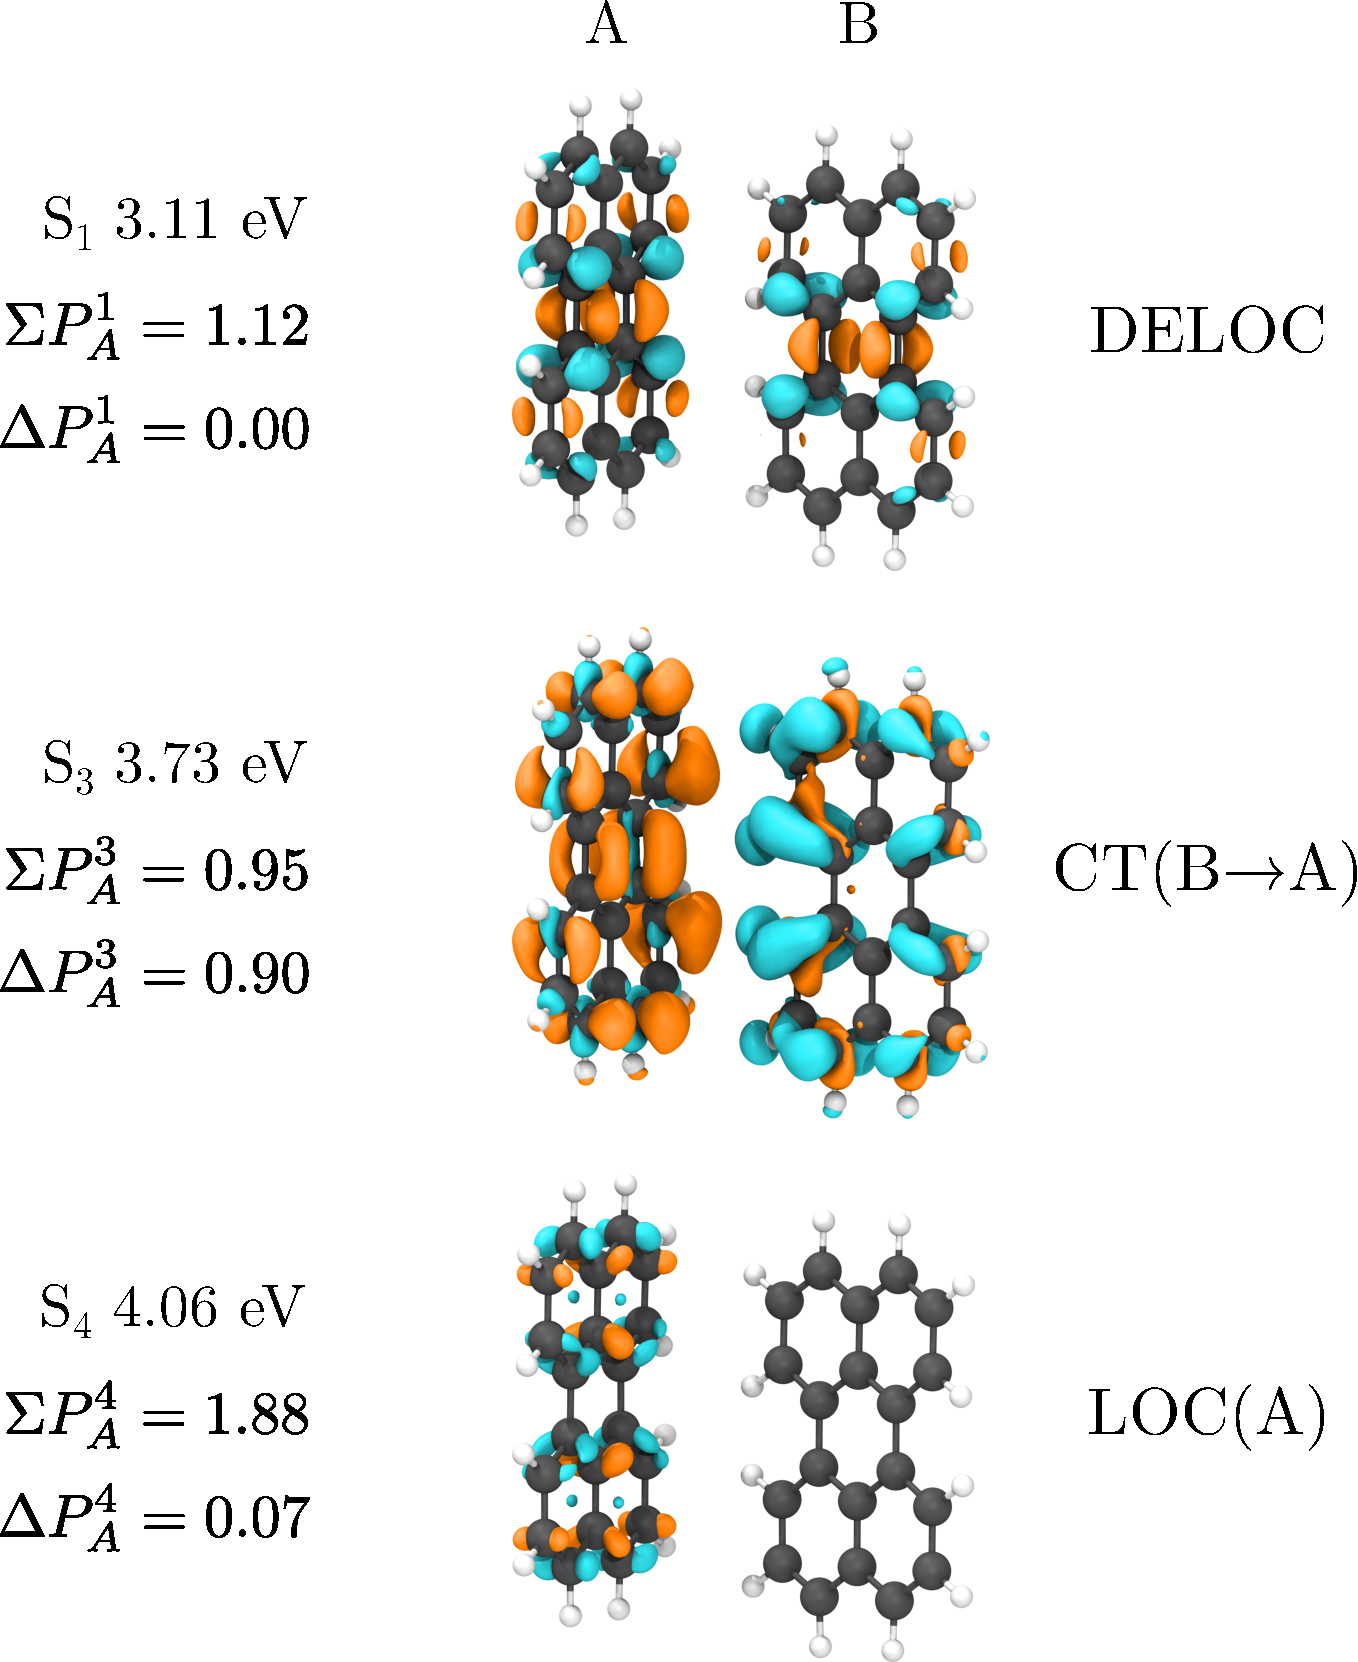
\includegraphics[width=7cm]{Chapters/6Implementation/classification.pdf}
  \caption{Transition density of two excited states of a perylene dimer taken from its crystal structure. The excited state energies are reported with respected to S$_0$. The electron density migrates from the blue to the yellow areas upon excitation. The exciton classification indices are defined in equation \ref{eq:exciton} and are in units of $\mathrm{e^-}$.}
  \label{fig:classification}
\end{figure}

To evaluate the two indices and classify an excitation, the user should first perform a TDDFT or CIS calculation of the dimer. Currently, only \texttt{Gaussian} calculations are supported. They should ensure that the atoms of molecule A appear before those of B in the geometry field and that an \texttt{rwf} file is produced by using the option \texttt{\%rwf=[name].rwf}. Then, given the output files \texttt{tddft.log} and \texttt{tddft.rwf}, the command line:
\begin{verbatim}
fro_exciton_classification.py tddft.log tddft.rwf [number of excitation]
\end{verbatim}
will print out the values of $\Sigma P^I_A$ and $\Delta P^I_A$ along with a suggested classification (\texttt{DELOC}, \texttt{LOC(A)}, \texttt{LOC(B)}, \texttt{CT(B→A)} and \texttt{CT(A→B)}).

To illustrate the use of this feature, a dimer of perylene was extracted from its experimental crystal structure.\cite{Botoshansky2003} Its excited states were calculated in \texttt{Gaussian16} using TD-$\omega$B97X-D\slash{}6-31G(d), and the transition densities analysed using the orbital specific Mulliken partition scheme. The states S$_3$ and S$_4$ each had extreme values of the classification indices, with $\Sigma P^3_A = 0.95$ $\mathrm{e^-}$ and $\Delta P^3_A = 0.90$ $\mathrm{e^-}$ for the former, indicating a charge transfer from fragment B to a, and $\Sigma P^4_A = 1.88$ $\mathrm{e^-}$ and $\Delta P^4_A = 0.07$ $\mathrm{e^-}$ for the latter, corresponding to a transition confined to monomer A. Figure \ref{fig:classification} corroborates this classification by showing the electronic transition density of a \texttt{DELOC} S$_1$ and comparing it to the \texttt{CT(B→A)} S$_3$ and \texttt{LOC(A)} S$_4$.




\subsubsection{Exciton Coupling Evaluation}
\label{sec:detail_js}
The coupling associated with an exciton is a measure of the correlation between the individual isolated excitations within the exciton. Evaluating it can give us a quantitative bearing on the importance of the many-body effects in the excited state process.

Kasha's exciton model is the initial approach, reducing the electronic densities of the fragments to point dipoles and comparing their relative geometry.\cite{Kasha1965} Under the point dipole approximation (PDA), the exciton coupling between fragments $i$ and $j$ is expressed as:
\begin{equation}
J_{ij}^{\text{Kasha}} = \frac{\bm{\mu_i} \bm{\mu_j}}{R^3} - \frac{3(\bm{\mu_i}\cdot{}\bm{R_{ij}})(\bm{R_{ij}} \cdot{} \bm{\mu_j}) }{R^5}
\label{eq:pda}
\end{equation}
Where $\bm{\mu_n}$ is the electronic transition dipole moment for monomer $n$ and $\bm{R_{ij}}$ is the vector connecting the centroids of monomers $i$ and $j$.

For a better spatial resolution of the electrostatic interactions, one can instead calculate the interaction between atomic transition charges (ATC)\cite{Spano2016}:
\begin{equation}
J_{ij}^{\text{ATC}} = \sum_a^{N_i}\sum_b^{M_j} \frac{q_a q_b}{|\bm{R_a^i} - \bm{R_b^j}|}
\label{eq:atc}
\end{equation}
Where $\bm{R_c^k}$ is the position of atom $c$ of monomer $k$ with ATC $q_c$ and $N_k$ is the number of atoms of monomer $k$.

For more resolution, the transition electronic density itself can be used, yielding costly but exact Coulombic exciton coupling. Additional correction can be included, for example by including the dielectric response of the environment as a polarisable continuum model as is done in \texttt{EXAT}.\cite{Jurinovich2018}

These models are purely Coulombic in nature and do not take into account the short-range interaction affecting the excited state behaviour of adjacent molecules, which for example is dominant in charge-transfer states.

Aragó and Troisi have devised a procedure which evaluates the coupling $J_{ij}$ in a dimer by diabatising the Hamiltonian:\cite{Arag2015}
\begin{enumerate}
    \item Select an excited state property. For the sake of argument we will use the transition dipole moment (TDM) $\bm{\mu}$ but anything bearing relation to the excited electronic density would be applicable.
    \item Evaluate the property for the two lowest excited states, along with the energies, for the dimer. These are the adiabatic energies ($E^A_1$ and $E^A_2$) and adiabatic TDMs ($\bm{\mu}^A_1$ and $\bm{\mu}^A_2$).
    \item Evaluate the property for both isolated constituent monomers in the first excited state, retaining their orientation. These TDMs are labelled $\bm{\mu}^{ISO}_1$ and $\bm{\mu}^{ISO}_2$.
    \item Calculate the singular value decomposition $(\bm{\mu}^A)^*\bm{\mu}^{ISO} = \bm{U}\bm{\Sigma}\bm{V}^*$.
    \item Compute the matrix $\bm{C} = (\bm{UV}^*)^*$ which is the best unitary transformation matrix mapping the adiabatic to the diabatic basis.
    \item Compute the diabatic Hamiltonian:
\begin{equation}
\small
\label{eq:2j}
\begin{pmatrix}
E_{i}^D & J_{ij}\\
J_{ji} & E_{j}^D
\end{pmatrix}
=
\begin{pmatrix}
C_{11} & C_{12}\\
C_{21} & C_{22}
\end{pmatrix}
\begin{pmatrix}
E_{i}^A & 0\\
0 & E_{j}^A
\end{pmatrix}
\begin{pmatrix}
C_{11} & C_{12}\\
C_{21} & C_{22}
\end{pmatrix}
\nonumber
\end{equation}     

\end{enumerate}

The off-diagonal elements of the Hamiltonian the exciton coupling values $J_{ij}$. More details can be found in reference \citenum{Arag2015}. The diabatisation method has already been employed in \texttt{fromage} to investigate the aggregate behaviour of propeller-shaped emitters.\cite{Stojanovic2019}

We have further extended it to calculate $N$-dimensional diabatic Hamiltonians, thus, for example, allowing for the calculation of pairwise exciton coupling within a trimer in the excited state, taking into account the influence of the third monomer.

An additional approximate method is that of exploiting the exciton energy splitting of the molecular excited state upon formation of a dimer. In the dimer, the S$_1$ and S$_2$ states are separated by twice the magnitude of the exciton coupling, provided that the individual constituent molecules are in perfect resonance.\cite{Hsu2009} Even in less symmetric cases, this approximation has been used with reasonable success.\cite{Gierschner2013,Shi2017,Dommett2019}

\texttt{fromage} implements this half-gap method, the PDA Kasha model, the ATC Coulombic interaction model and the diabatisation scheme using either ATCs or TDMs as excited state properties.

The script \texttt{fro\_coupling.py} manipulates \texttt{Gaussian} log files to compute exciton couplings. Several schemes are implemented. For instance, if a user requires the diabatisation method using the TDM excited state property to find the diabatic Hamiltonian containing the first three couplings of a trimer, the steps would be as follows. Carry out \texttt{Gaussian} calculations of the S$_1$ states of the three constituent monomers and the first three excited states of the trimer, yielding the files \texttt{mon\_1.log mon\_2.log mon\_3.log} and \texttt{trim.log}. Then, use the command line:
\begin{verbatim}
fro_coupling.py -m DIA -p TDM -mf mon_1.log mon_2.log mon_3.log -nf trim.log -ns 3
\end{verbatim}

This will print out the diabatic Hamiltonian where the three lower triangular off-diagonal elements correspond to the three exciton couplings of the trimer.

As an illustrative example, the crystal structure of 1,4-bis-(4-styryl-styryl)-benzene (4PV) was used to extract inequivalent dimers and evaluate their couplings. The structure of 4PV has been experimentally shown to contain six monomers, departing from the high symmetry of an ideal herringbone crystal due to variable slight rotation of the extreme phenyl rings.\cite{VanHutten1999} First, the unit cell was optimised using PBE-D2 with a basis set cut-off of 50 Ry and a Monkhorst-Pack grid of 1x2x1 k-points as implemented in \texttt{Quantum Espresso}.\cite{Giannozzi2009} Then, the inequivalent dimers were detected by \texttt{fromage} using a centroid-centroid distance threshold of 7 \AA. The TDMs of these dimers were calculated using TD-$\omega$B97X-D\slash{}6-31G(d) in \texttt{Gaussian16}\cite{g16} and processed in \texttt{fromage} in order to evaluate exciton couplings using dimer and trimer diabatic Hamiltonians. The results are shown in Figure \ref{fig:4pv}. In this system, edge-to-face dimer arrangements have larger exciton couplings (97, 103 and 105 meV) than face-to-face ones (79 and 91 meV). The largest difference is of 26 meV which represents 25\% of the greatest coupling (105 meV). It is expected that in cofacial dimers with couplings of such magnitude, the short-range interactions should account for most of the coupling, making the use of a coupling scheme which accounts for exchange imperative.\cite{Fornari2017}

Overall, the inclusion of the third molecule in the trimer diabatic Hamiltonian reduces the magnitude of the couplings by about 10 meV which is significant since it is in the order of the difference between certain edge-to-face and face-to-face values.

The irregularities in the herringbone packing produce two different face-to-face dimers with respective centroid-centroid distances of 6.05 \AA{} and 6.15 \AA{}. This relatively small increase in distance reduces the exciton coupling by 12 meV (14\% of the average value), indicating that the natural packing of 4PV produces in dimers in an excitonically sensitive geometry.

\begin{figure}[ht]
\centering
  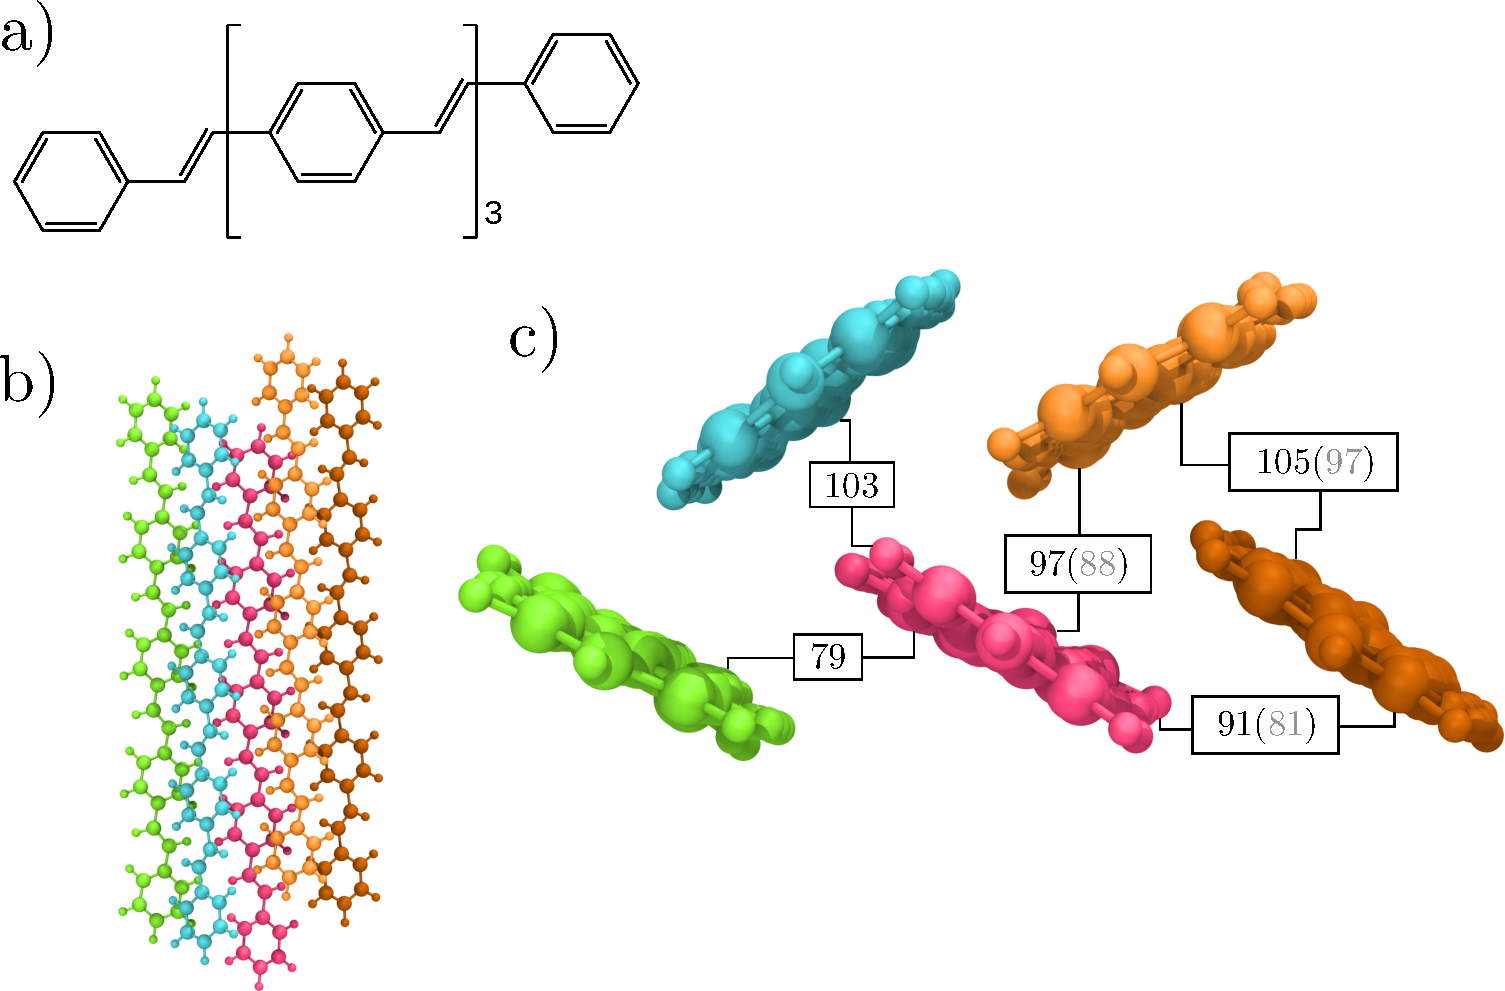
\includegraphics[width=11cm]{Chapters/6Implementation/dimer_js.pdf}
  \caption{a) Chemical structure of 4PV b) Top view of a cluster of 4PV molecules taken from their crystal positions c) Side view of the cluster with inequivalent dimers labelled by their exciton coupling value in meV. The values in parentheses are calculated as a trimer.}
  \label{fig:4pv}
\end{figure}

% In a trimer chromophore, $\textbf{H}^D$ becomes a 3x3 matrix
% \begin{equation}
% \small
% \label{equation: 3x3 diabatic matrix}
% \begin{bmatrix}
% E_{i}^D & J_{ij} & J_{ik}\\
% J_{ji} & E_{j}^D & J_{jk} \\
% J_{ki} & J_{kj}& E_{k}^D
% \end{bmatrix}
% =
% \begin{bmatrix}
% C_{11} & C_{12} & C_{13}\\
% C_{21} & C_{22} & C_{23}\\
% C_{31} & C_{32} & C_{33}
% \end{bmatrix}
% \begin{bmatrix}
% E_{i}^A & 0 & 0\\
% 0 & E_{j}^A & 0\\
% 0 & 0 & E_{k}^A\\
% \end{bmatrix}
% \begin{bmatrix}
% C_{11} & C_{12} & C_{13}\\
% C_{21} & C_{22} & C_{23}\\
% C_{31} & C_{32} & C_{33}
% \end{bmatrix}
% \end{equation} 


\subsection{ONIOM Calculations}
\label{sec:prog_oniom}
Whether it be to calculate an absorption or emission energy, locate nonradiative pathways, or build a potential energy surface, calculating an excited state electronic structure is an often unavoidable step in the study of molecular aggregates. This often proves to be challenging due to the environmental effects in such media.

As discussed in Chapter \ref{chap:emb}, hybrid method schemes can offer environmental corrections, where an active site calculated with a high accuracy method is embedded in an explicit environment of lower accuracy. Inter-program hybrid method codes are not uncommon. \texttt{GARLEEK}\cite{Pedregal2018} communicates between \texttt{Gaussian} and \texttt{Tinker} for subtractive QM:MM calculations. \texttt{Chemshell}\cite{Metz2014,Lu2019} provides additive QM:MM formulations. The Atomic Simulation Environment (ASE)\cite{Larsen2017} offers both additive and subtractive QM:MM as a Python library. However to our knowledge no such code yet offers inter-program ONIOM QM:QM' calculations in the excited state. \texttt{fromage} uses its interfaces with \texttt{DFTB+}, \texttt{Gaussian}, \texttt{Molcas}, and \texttt{Turbomole} to calculate energies and geometry optimisations of different kinds with ONIOM QM:QM'. Namely mechanical embedding, regular electrostatic embedding, Ewald point charge embedding, and self-consistent versions of the last two.

The point charges can originate from Mulliken or RESP calculations. To fit point charges to the Ewald potential, we use the \texttt{Ewald} program.\cite{Klintenberg2000,Derenzo2000,Weber2010} It was modified to allow for the use of noninteger charges and redistributed at \href{https://github.com/Crespo-Otero-group/Ewald}{https://github.com/Crespo-Otero-group/Ewald} with permission from the original authors, fulfilling the requirements of the Computer Physics Communications license.

The various quantum methods available and tested in \texttt{fromage} are listed in Table \ref{tab:methods} along with their corresponding programs.
\begin{table}
\centering
\caption{Interfaced quantum methods and their availability in electronic structure programs}
\begin{tabular}{lcccc}
    \toprule
    Method & DFTB+ & Gaussian & Molcas & Turbomole \\\midrule
    Hartree-Fock & \xmark & \textcolor[HTML]{589A21}{\cmark} & \xmark & \textcolor[HTML]{589A21}{\cmark}\\
    DFTB & \textcolor[HTML]{589A21}{\cmark} & \xmark & \xmark & \xmark\\
    DFT & \xmark & \textcolor[HTML]{589A21}{\cmark} & \xmark & \textcolor[HTML]{589A21}{\cmark}\\
    TDDFT & \xmark & \textcolor[HTML]{589A21}{\cmark} & \xmark & \textcolor[HTML]{589A21}{\cmark}\\
    ADC(2) & \xmark & \xmark & \xmark & \textcolor[HTML]{589A21}{\cmark}\\
    CC2 & \xmark & \xmark & \xmark & \textcolor[HTML]{589A21}{\cmark}\\
    CASSCF & \xmark & \textcolor[HTML]{589A21}{\cmark} & \textcolor[HTML]{589A21}{\cmark} & \xmark\\
    CASPT2 & \xmark & \xmark & \textcolor[HTML]{589A21}{\cmark} & \xmark\\\bottomrule
    \label{tab:methods}
\end{tabular}
\end{table}


Setting up hybrid method calculations is typically a technically tedious task, but as many steps as possible are automated in \texttt{fromage} while retaining the full flexibility of the interfacing programs. The line:
\begin{verbatim}
fro_prep_run.py
\end{verbatim}
accompanied with a few input files such as the unit cell and a configuration file, will prepare the template files for the actual calculations to follow. This may include cluster geometry generation, Ewald fitting procedures and self-consistent population analyses.

Then, if the user is satisfied with their newly generated embedded cluster, the line:
\begin{verbatim}
fro_run.py
\end{verbatim}
can perform geometry optimisation or single point calculations.

OEC, OEEC and SC-OEEC calculations all require the distribution of point charges from single molecule population analyses to aggregate geometries or unit cell structures. This is a routine operation for preparing forcefield calculations, where sets of atomic types are associated to a potential or another with predetermined charge values.\cite{Wang2004,Wang2006} The atomic type is usually dependent on its neighbouring bonded atoms and the bond types. For QM:QM' calculations, it would be more attractive to use a broader definition of the atomic type which distinguishes between same function atoms at nonequivalent parts of the molecule.

To this end, \texttt{fromage} implements a connectivity detection tool which reads population analysis information from a single molecule or unit cell calculation and redistributes it onto any other finite or periodic ensemble of same molecules. The procedure builds a bond order matrix $\mathbf{B}$ where $B_{ij}$ is the shortest path connecting atoms $i$ to $j$ in number of bonds. The construction of the matrix is represented in Figure \ref{fig:connectivity} and is performed as follows:
\begin{enumerate}
  \item Detect the first connections by computing all of the interatomic distances complemented by atomic radii.
  \item Check every zero element and detect atom pairs $(a,b)$ which have a connected atom $c$ in common, i.e. $B_{ac} \neq 0 \land B_{bc} \neq 0$.
  \item Assign $B_{ab} = B_{ac} + B_{bc}$.
  \item Repeat from step 2 until convergence of the matrix.
\end{enumerate}

An atom's identity can be completely defined by additionally using the element of the atom corresponding to each row of $\textbf{B}$. A sufficient fingerprint for a given atom is the amount of atoms of a given element which are located a certain amount of bonds away, accompanied by the atom's own element. For example a methyl hydrogen of methanol is sufficiently defined by stating that it is a hydrogen atom with one carbon atom one bond away, one oxygen atom two bonds away, two hydrogen atoms two bonds away and one hydrogen atom three bonds away.


\begin{figure}[ht]
\centering
  \includegraphics[width=\textwidth]{Chapters/6Implementation/matrices.pdf}
  \caption{Generation of the bond order matrix for methanol.}
  \label{fig:connectivity}
\end{figure}

Once all of the atomic identities are sampled from a reference molecule or unit cell, the partial charge values from this reference are distributed onto the desired target. When several reference atoms have the same identity (for instance three hydrogens belonging to the same methyl group), the average charge is retained. In practical terms, given for instance a Mulliken population analysis of methanol calculated in \texttt{Gaussian} with output file \texttt{pop.log}, and a Cartesian coordinate file of a cluster of methanol molecules \texttt{clust.xyz}, the line:

\begin{verbatim}
fro_assign_charges.py pop.log clust.xyz
\end{verbatim}
will produce a file \texttt{out\_char} which contains the coordinates of \texttt{clust.xyz} with an added column stating the partial charge of each atom.

All geometry optimisation routines use the the BFGS algorithm as implemented in \texttt{scipy}.\cite{scipy} To locate minima on the PES, the ONIOM energy expression (Equation \ref{eq:imomo}) is minimised. To locate conical intersections, the penalty function of Levine, Coe, and Mart\'inez is used instead (see Section \ref{sec:theo}).\cite{Levine2008}

\subsubsection{Example of Use}

The optimisation of excited state geometries in detailed condensed phase environments has numerous applications. For instance, the fluorescence of HC1 (see section \ref{sec:vor}) can also be switched off by the substitution of a methyl group in \textit{para} position with respect to the hydroxyl group, resulting in another dark compound: (2E)-3-[4-(Dimethylamino)phenyl]-1-(2-hydroxy-5-methylphenyl)-2-propen-1-one (DMAP).\cite{Zhang2015,Zahid2017}

Both HC1 and DMAP can experience excited state intramolecular proton transfer, splitting the excited state into two potential decay pathways. It was recently computationally shown that in HC, both the enol and the keto non-radiative decay pathways were rendered energetically inaccessible by a combination of molecular and crystalline factors.\cite{Dommett2017a,Dommett2017c}

OEEC was employed to investigate the critical points in the potential energy surface of DMAP. A thorough tutorial on how to perform these calculations is available here: \href{https://fromage.readthedocs.io/en/latest/tutorial.html}{https://fromage.readthedocs.io/en/latest/tutorial.html}. Geometry optimisations were carried out to locate the ground and excited state minima, as well as its Minimal Energy Conical Intersection Geometries (MECI). The crystal structure was optimised in \texttt{Quantum Espresso} using PBE-D2, a 40 Ry basis cutoff and a 1x2x1 k-point mesh. For the ONIOM calculation, the QM level of theory was TD-$\omega$B97X-D/6-311++G(d,p) while for the QM' level of theory, both HF/STO-3G and DFTB were employed. The energies and gradients were computed in \texttt{Gaussian16} for TDDFT and HF and in \texttt{DFTB+} for DFTB. Figure \ref{fig:pes_hc4} shows the relative energies of all the optimised critical points of the PES.

\begin{figure}[ht]
\centering
  \includegraphics[width=6.5cm]{Chapters/6Implementation/hc4_fig.pdf}
  \caption{Relative energies of critical geometries of DMAP evaluated with OEEC at critical points of the PES. The Franck\textendash{}Condon point (FC), Enol (E*) and Keto (K*) excited state minima and Conical Intersection (CI) geometries were located.}
  \label{fig:pes_hc4}
\end{figure}

The enol non-radiative decay pathway is significantly above the absorption energy, rendering this channel inaccessible. On the other hand, the keto conical intersection is only about 0.2 eV above the absorption energy, arguably making it accessible \textit{via} thermal fluctuations. The availability of this nonradiative decay channel explains the low fluorescence quantum yield.

The TDDFT:HF and TDDFT:DFTB levels of theory have similar results, both in geometry and energy, with a difference of less than 0.1 eV at each point except form the enol MECI. This outlier can be attributed to the extreme bond stretching occurring between carbons in the back bond in the enol MECI conformation which would render both the Hartree-Fock formalism and the parameterisation of the DFTB calculations inadequate in differing ways. The striking agreement between the two methods is encouraging, given the relatively low computational cost of the semiempirical computation and the prevalence of HF as a ground state theory in QM:QM' protocols.\cite{Presti2014,Presti2016,Presti2016a,Presti2017}





\section{Conclusion}
We have detailed the principal capabilities of the Python library \texttt{fromage}, which aims to facilitate the computational investigation of the excited states of molecular aggregates. They include geometrical and exciton analysis as well as QM:QM' geometry optimisation tools, which have already been successfully employed in three past publications.\cite{Rivera2019,Stojanovic2019,Dommett2019} The features were tested on a diverse array of molecules, in order to challenge their robustness. They are implemented with enough flexibility that Python literate researchers can employ \texttt{fromage} scripts as part of a larger workflow with little added effort. By virtue of being an open source, unit tested and documented piece of software, \texttt{fromage} represents an addition to the fast expanding pool of sustainable chemical software libraries. We hope that by enabling researchers to use the framework and manipulate the source code, the field of aggregate photochemistry will continue to mature towards modern reproducible workflows.
\chapter{Application}
\label{chap:molecules}
\section{Introduction}

With the new suite of tools implemented in \texttt{fromage}, we now focus on applying them to increasingly diverse systems, in the hope to glean some chemical insight. The objective is both to provide robustness to the program, whilst studying the properties of emissive organic molecular crystals .

To fully control the luminescent behaviour of these materials, the excited state radiative and non-radiative decay channels of the molecule need to be understood within a particular condensed phase environment. Despite the abundance in experimental and theoretical investigations of the excited states of molecular crystals, understanding these decay channels is still extremely challenging, and is done on a case-by-case basis for newly discovered compounds. The main obstacle to generalising design rules for these materials is the interconnectedness of their defining properties at the molecular and intermolecular levels.

In this chapter, we analyse the role of different factors affecting the emissive response of thirteen luminescent molecular crystals, which have previously been characterised experimentally (Figure \ref{fig:molecules_app}). We aim to consider a large enough variety of systems that comparisons can be drawn between crystals with different degrees of packing and chemical similarity. \miguel{Our main focus is to rationalise the Quantum Efficiency of Fluorescence (QEF) of these materials as a competition between radiative and nonradiative decay channels, arising from different inter- and intramolecular factors. We consider a diverse enough range of materials to highlight how differently behaving solute molecules can arrive at the same desirable emissive property in the crystal phase.}

\begin{figure}
\centering
\includegraphics[width=9cm]{Chapters/7Applications/molecules.pdf}
\caption{Molecular structures of the studied systems.}
\label{fig:molecules_app}
\end{figure}
%%%

The crystals were gathered into series based on their backbone structures and substituents. p-oligophenylenes ($n$P, $n$=3, 4, and 6) are a family of organic $\pi-$conjugated molecules composed of phenyl-rings attached to each other via single bonds in para-positions. The DCS series where three phenylene units are connected by vinylene bridges with cyano-group substituents, and additional buthoxy and methoxy groups are added to the backbone. We also consider the DSB molecule, which shares the same backbone but has no substituents and 4PV which further extends the phenylene chain by two phenylene units. Additionally, we consider 2-(2'-hydroxyphenyl)benzothiazole (HBT), a molecule exhibiting excited state proton transfer in the solid state. All molecules are represented on Figure \ref{fig:molecules}.

% Bogatko2016 says that the absorption of acenes goes down with length

Barring certain substitutions of the DCS family and HBT, all systems display amplified spontaneous emission (ASE) in crystal, making them candidates for use as organic single crystal lasers, as detailed in Reference \citenum{Gierschner2016}. All molecules undergo Solid State Luminescence (SSL),\cite{Shi2017} some of it induced by crystallisation\textemdash{}Solid State Luminescence Enhancement (SLE).


%%%

%%Throwing some ideas around
We first present the computational details of our findings. Then, in order to understand the emissive behaviour of the crystals, we analyse  the geometric features of the crystal packing, the excitonic coupling between constituent dimers, and the energetics of the excited states along critical points of their potential energy surfaces. We conclude by comparing the findings between series and assessing the efficacy of our available analysis methods in \miguel{elucidating competing radiative and nonradiative mechanisms}.


\section{Computational Details}
The crystal structure geometries were optimised using PBE-D2 as implemented in \texttt{Quantum Espresso}\cite{Giannozzi2009}, with a basis set cut-off of 50 Ry and various Monkhorst-Pack Grids chosen in accordance with the unit cell shapes.

The investigation of the multiple molecules was facilitated by the recent development of \texttt{fromage}, a Python library dedicated to studying excited state molecular aggregates and crystals. This work showcases the robustness of its features by applying geometry analysis tools, excitonic coupling evaluation, and ONIOM methods to the crystals.

In order to isolate dimers from the lattice, a spherical molecular cluster was extracted from the crystal, and its pairs of molecules with with intermolecular contacts smaller than 4 \AA{} were selected. Then, the intermolecular atomic distances of each dimer were evaluated and sorted so as to provide a fingerprint for the dimer configuration. These distances were finally compared between dimers and if their RMSD fell below $10^{-4}$ \AA, the dimers were considered identical and only one was preserved.

To characterise the configurations of the unique dimers, an orthonormal pair of principal and secondary axes was calculated for each constituent fragment, and the angles between same axes of two molecules was evaluated. To obtain the vectors, first, all atoms of the molecule were projected onto an averaged plane via singular value decomposition. The principal axis was defined as the vector tracing the longest interatomic distance and the secondary axis its perpendicular vector on the averaged plane.\cite{Rivera2020} This process is represented for a dimer of the 3P crystal in Figure \ref{fig:axes}.

\begin{figure}
\centering
\includegraphics[width=6cm]{Chapters/7Applications/axes.pdf}
\caption{a) Principal and secondary axes on the 3P monomer b) Top view of a 3P dimer c) Side view of the same dimer.}
\label{fig:axes}
\end{figure}

All molecules have rotational symmetry about both of the axes when defined this way apart from HBT which has an inherent orientation. In the case of this molecule, we employed the scheme described in Section \ref{sec:dimer_axes} where, by exploiting the two longest interatomic distances on the averaged plane, a set of axes could be defined with consistent orientation.

To evaluate exciton couplings between dimers, the diabatisation scheme by Troisi and Arag\'o\cite{Arag2015}, as implemented in \texttt{fromage}. The transition dipole moments of the isolated monomers were compared to those in the dimer to construct a diabatic Hamiltonian, whose off-diagonal elements are the exciton couplings. The original algorithm is thoroughly described in the Supporting Information of Reference \citenum{Arag2015} and in reference \citenum{Rivera2020}. The transition dipole moments were calculated in \texttt{Gaussian}\cite{g16} using TD-$\omega$B97X-D/6-31G(d).

For QM:QM' calculations, the ONIOM scheme was used, using electrostatic embedding. The excited state level of theory was TDDFT $\omega$B97X-D/6-31G(d), with \texttt{Gaussian}, or ADC(2)/SV(P), with \texttt{Turbomole}\cite{TURBOMOLE}. The high level region was embedded in point charges from RESP calculations of DFT $\omega$B97X-D/6-31G(d) calculated in \texttt{Gaussian}. For the polar molecules HBT and $\alpha$-DCS, the electrostatic embedding was extended to include long range Coulomb interactions using the ONIOM Ewald Embedded Cluster method (OEEC).\cite{Rivera2019} The ground state level of theory was DFTB, with \texttt{DFTB+}\cite{Aradi2007}, and the embedding for the central region was done using RESP calculations with PBE/6-31G(d) calculated in \texttt{Gaussian}. Multireference SA-2-CASSCF and MS-2-CASPT2 calculations were performed with Molcas.\cite{Aquilante2016} The active spaces are reported in the Supplementary Information.

\miguel{To sample the exciton coupling of in the dimeric vibrational space of the crystal, the QM:QM' calculations were carried out on dimers to find their FC point. Then, a normal modes calculation was carried out, from which a Wigner distribution of 200 sample geometries were extracted using \texttt{Newton-X}.\cite{Crespo-Otero2012,Barbatti2014} The exciton couplings were then evaluated using the diabatisation method.}

The Huang-Rhys factors (S$_i$) for relaxation within the S$_1$ state, between S$_0$ and S$_1$ minima, were evaluated for the members of $n$P and DCS series in vacuum and crystal environment using the \texttt{DUSHIN} code.\cite{Reimers2001AMolecules} The computations were based on normal modes computed at the optimised S$_0$ and S$_1$ geometries in vacuum at the (TD-)$\omega$B97XD/6-31G(d) level and in crystal at the QM:QM' level described above. Reorganisation energies ($\lambda_i$) decomposed into normal mode contributions are related to Huang-Rhys factors as follows: 

\begin{equation}
\lambda_i = \hbar \omega_i S_i
\label{eq_hr}
\end{equation}

The Einstein\cite{Crespo-Otero2012} and Strickler-Berg\cite{SBrelation} (SB) relations were employed to evaluate radiative rates and lifetimes of selected fluorophores in solution and crystal. Einstein equation for spontaneous decay relates fluorescence rate ($k_r$) with emission energy ($\Delta E$) and oscillator strength ($f$).

\begin{equation}
k_r=\frac{2\Delta E f}{c^3}
\label{eq1}
\end{equation}

The SB relation takes into account transitions between vibronic wave functions of excited and ground states\cite{SBrelation}. According to the SB relation, the radiative rate can be evaluated as\cite{Shi2017}

\begin{equation}
k_r=0.667 [cm^2 \times s^{-1}] \frac{\nu_F^3}{\nu_A}n^2 f
\label{eq2}
\end{equation}
Where $\nu_F$ and $\nu_A$ are vertical emission and absorption energies (in $cm^{-1}$), $f$ is the oscillator strength, and $n$ is the refractive index of a solvent.

% \textcolor{blue}{(RCO: - we need here the description of the models we are using for the crystals. We also need to specify the QM:QM' methods we are considering)} 


To evaluate exciton hopping rates, the Marcus scheme was employed:
\begin{equation}
\nu_{ij}=\frac{J_{ij}^2}{\hbar}\sqrt{\frac{\pi}{\lambda k_{\text{B}}T}}\exp\bigg[-\frac{\lambda}{4k_{\text{{B}}}T}\bigg]
\label{eq:marcus}
\end{equation}
Where $J_{ij}$ is the exciton coupling between excited monomers, $\hbar$ is the reduced Planck's constant, $k_\text{B}$ is Planck's constant, $\lambda$ is the reorganisation energy computed as described above, and $T$ is room temperature of 298 K.\cite{Stehr2014,Kimura2000}
\section{Results}

\subsection{Dimeric Arrangement}
Due to the non-covalent nature of molecular crystals, photophenomena often occur locally\cite{Arag2015} and can be understood on the scale of the nearest neighbour molecules. In particular, the conformational features of the dimer arrangements resulting from the packing of the crystal can elucidate the pairwise interactions affecting the excited states in the crystal.

The packing motifs of these materials are diverse and smoothly varying, making them challenging to classify. However certain patterns have been identified to occur frequently, and we use these as reference points.\cite{Desiraju1989,Campbell2017} In particular, herringbone crystals pack in an alternating edge-to-face arrangement, while sheet crystals have all molecules sharing the same orientation arranged in regular layers. These two motifs are represented in Figure \ref{fig:packing}. \miguel{For the sake of clarity, in this chapter, we employ the terms like \textit{herringbone} and \textit{sheet} to refer to the overall crystal packing, and ones like \textit{edge-to-face} or \textit{face-to-face} to denote specific dimer arrangements.}

\miguel{Table \ref{tab:molecules} summarises the principal data relating to the packing and emission of all systems. We immediately note the prevalence of H dimers arising from the herringbone and sheet packing patterns, which result in significant QEF values, contradicting Kasha's exciton model.\cite{Kasha1965} The intermolecular processes in these materials therefore must go beyond point-dipole approximations.}

\begin{figure}
\centering12
\includegraphics[width=7cm]{Chapters/7Applications/packings.pdf}
\caption{Illustration of two archetypal packing motifs in molecular crystals.}
\label{fig:packing}
\end{figure}

The significant dimers of the crystals in consideration were processed in \texttt{fromage} to extract their characteristic angles. The overall crystal packing was found to be split between the series of molecules. The DCS series primarily forms sheets, while the other crystals have a clear bias towards herringbone motifs. The principal axis angles in face-to-face dimers of sheet crystals are almost always 0\degree{} due to the translational symmetry between layers. In contrast, herringbone crystals usually have nearly parallel principal axes and a large array of secondary axis angles. Indeed the tilt between herringbone layers is strongly dependent on the morphology of the constituent fragments.

\begin{figure}
\centering
\includegraphics[width=9cm]{Chapters/7Applications/angles.pdf}
\caption{Distribution of the dimeric arrangements in the DCS series (14 dimers) and the rest of the crystals (14 dimers). The angle between principal axes is plotted against the angle of the secondary axes. Almost all DCS series dimers are perfectly parallel, the exceptions are shown.}
\label{fig:angles}
\end{figure}


The angle values for non-DCS series crystals are represented as a density map in Figure \ref{fig:angles}. The herringbone and sheet families of crystals can be spotted by their characteristic densities centred around (0\degree{},0\degree{}) and (60\degree{},15\degree{}) respectively. Herringbone crystals also contribute to the density at (0\degree{},0\degree{}), given that they are made up not only of edge-to-face dimers but also of face-to-face ones. Furthermore, there is more configurational variety in edge-to-face dimers, as evidenced by the wide spread of $beta$ angles. The island of dimers of $\alpha$ angles larger than 10\degree{} is due only to one 4PV dimer and two HBT dimers. This slight departure from ideal herringbone packing is known in 4PV\cite{VanHutten1999}, where the unit cell includes six molecules instead of two. HBT displays slightly misaligned head-to-tail dimers indicating that each layer of the material in the principal axis direction has an alternating orientation.

The DCS series dimers are represented as a points on the same plot. All of the points were found at the (0\degree{},0\degree{}) position, except for four outliers. DSB has a dimer at (1.2\degree{},58.9\degree{}), which is near the centre of the dense shaded area. This confirms the nature of DSB as a herringbone crystal, which becomes a sheet crystal only following substitutions. $\alpha$-DCS and $\beta$-DBDCS have dimers at (1.3\degree{},24.9\degree{}) and (2.3\degree{},13.5\degree{}) respectively, which break the translational symmetry due to the freedom of rotation of their central aromatic ring. $\alpha$-MODCS has a point at (38.5\degree{},10.3\degree{}), which is far away from any other considered dimer. The packing of this crystal does not match any of the common packing classifications.

\subsection{Exciton Coupling}
The values of the exciton couplings of the molecules under scrutiny, evaluated at their Frank-Condon region, are a result of structural and chemical features of the dimers formed upon aggregation. We therefore wish to highlight any possible correlations between the packing patterns described above, and the exciton states within the crystal. These states are liable to cause delocalised excitation phenomena, discouraging emission.

We first examine the dependence of the couplings on the distance between constituent fragments of the dimer. Figure \ref{fig:dist} shows the exciton coupling of each dimer of the crystal structures with respect to the centroid-to-centroid distance of said dimer. We observe a clear monotonic downward trend for dimers belonging to every crystal except for HBT. This trend is in line with the limiting behaviour where fragments become non interacting at infinite distances and the coupling should therefore tend to zero. In the middle to long range, the electrostatic interaction between the two fragments approaches a $1/r$ shape where $r$ is the distance between the centres of mass of each electron could. Figure \ref{fig:dist} does not have the sufficient resolution to suggest an inverse law as opposed to other monotonically decreasing functions. However, we can observe that dimers from different series have similar exciton coupling given similar centroid-to-centroid distance \miguel{within a range of 50 meV. This is a surprising result because of the inadequacy of centroid distance as a measure of correlation of neighbouring excited states, ignoring the shape of the molecular wavefunctions altogether.}

\begin{figure} [h!]
\centering
\includegraphics[width=8cm]{Chapters/7Applications/dist_coupling.pdf}
\caption{(top) Exciton coupling (J) as a function of the centroid-to-centroid distance of the constituent monomers of each dimer. The values of every dimer are fitted to an inverse law $f(r) = a/r$ \textit{via} least squares. The resulting function, with $a=459$ is plotted in pink and has a standard deviation of 27, represented by the shaded area. A dashed line represents the same fit but using an aromatic carbon (bottom) as a reference for the distance calculation, denoted HBT*. In this case, $a=480$ and the standard deviation is 23.}
\label{fig:dist}
\end{figure}

HBT constitutes a striking exception, where all of the nearest neighbour dimers have exciton coupling values between 20 and 40 meV. In particular, the two closest dimers, with centroid distances close to 5 \AA{}, are about 60 meV below the fit line. The transition densities of these dimers, compared with the monomer transition density are depicted in Figure \ref{fig:hbt_dens}. The excitation of the isolated molecule is mainly localised in the proton transfer moiety, breaking the apparent symmetry of the two constituent rings. Both closest dimer arrangements are aligned in centroid but opposite oriented, effectively distancing the excitation densities. This effect is less pronounced in other molecules because they are all symmetric in orientation of their long axis. By measuring the distance between HBT molecules with an aromatic carbon as a reference point, the exciton coupling values adopt a clearer downward trend, albeit shifted lower than for the other series.

\begin{figure}
\centering
\includegraphics[width=9cm]{Chapters/7Applications/hbt_dens.pdf}
\caption{Transition densities of the bright states of HBT in monomer form and both dimers of least centroid-to-centroid distance. Upon excitation, the density is reorganised from the blue to the orange areas.}
\label{fig:hbt_dens}
\end{figure}

Excluding HBT, the dimers are roughly split into two group, those below 7 \AA{} in separation, with couplings ranging from 82 to 140 meV and those above 7 \AA{} with couplings from 24 to 64 meV. Those in the former group are overall above the $a/r$ trend line, and those of the latter below. This may be explained by the added proportion of exciton coupling resulting from exchange in the strong coupling regime. Ref. \citenum{Fornari2017} found that when Coulombic coupling exceeds 70 meV in organic semiconductor materials and light-harvesting complexes, the exchange portion of the coupling always shares a sign with its electrostatic counterpart, thus increasing the total coupling. This is consistent with the deviation of the limiting behaviour of the total coupling from a Coulombic inverse law.

\begin{figure}
\centering
\includegraphics[width=8cm]{Chapters/7Applications/hist.pdf}
\caption{Exciton coupling values of irregularly packed DSB dimers, sampled from their vibrational phase space.}
\label{fig:hist}
\end{figure}


\begin{table*}
\scalebox{0.7}{
\begin{tabular}{@{}lccccccccccc@{}}

%\begin{tabular}{@{}llllllllllll@{}}
\toprule
\multirow{2}{*}{Crystal}    & \multirow{2}{*}{Series}  & \multirow{2}{*}{$V_i$} & \multirow{2}{*}{J (meV)$^a$} &   \multirow{2}{*}{Packing$^b$}  & \multirow{2}{*}{H dimer \%$^c$} & \multicolumn{3}{c}{Calculated absorption}& \multirow{2}{*}{Exp. absorption} & \multirow{2}{*}{$\Phi_f$}\\
& & & & & & Monomer & Dimer S$_1$ & Dimer S$_2$ &  & \\\midrule

%& E S1 dimer & E S2 dimer &   \\ 
DSB        & - & 1.41         & 131       & HB     & 100      & 3.60      & 3.47       & 3.65       & 3.48$^d$\cite{Shi2017}                        & 0.78          \\
4PV        & - & 1.42         & 103       & HB    & 100       & 3.10      & 2.98       & 3.19       &                -             & -           \\
HBT        & -     & 1.43         & 36       & HB & 83 & 3.98      & 3.94       & 4.00       & 3.65$^e$\cite{Lee2013}                  &  0.77$^g$\cite{hbt_exp}  \\
3P         & $n$P      & 1.37         & 98        & HB    & 100       & 4.36      & 4.24       & 4.43       & 4.51$^d$\cite{Pavlopoulos1974}                         & 0.67\cite{Katoh2009}          \\
4P         & $n$P      & 1.39         & 99        & HB    & 100       & 4.16      & 4.05       & 4.23       & 4.13$^d$\cite{Pavlopoulos1974}                         & -           \\
6P         & $n$P      & 2.27          & 95        & HB    & 100       & 3.75      & 3.63       & 3.82       &                  -           & 0.30$^h$\cite{6P_qy}  \\
$\alpha$-DCS     & DCS     & 1.41         & 97        & S      & 100   & 3.74      & 3.60       & 3.80       & 3.61$^f$\cite{Shi2017} & 0.90\\
$\alpha$-DBDCS   & DCS     & 1.49         & 53        & S  & 100   & 3.33      & 3.19       & 3.30       & 3.34$^f$\cite{Shi2017}                         & 0.62          \\
$\beta$-DBDCS   & DCS     & 1.53         & 113       & S  & 100 &  3.30      & 3.17       & 3.34       & 3.19$^f$\cite{Shi2017}                        & 0.84          \\
$\alpha$-MODCS   & DCS     & 1.42         & 32        & -  & 50 & 3.66      & 3.64       & 3.69       & 3.45$^e$\cite{Shi2017}                        & 0.66          \\
$\beta$-MODCS   & DCS     & 1.39         & 140       & S   & 100  & 3.06      & 2.86       & 3.13       & 2.95 3.60$^f$\cite{Shi2017}                   & 0.73          \\
$\alpha$-MODBDCS & DCS     & 1.44         & 103       & S   & 100  & 3.27      & 3.22       & 3.29       & 3.43 3.84$^f$\cite{Shi2017}                   & 0.42          \\
$\beta$-MODBDCS & DCS     & 1.43         & 121       & S   & 100  & 2.80      & 2.68       & 2.84       & 2.87 3.40$^f$\cite{Shi2017}                   & 0.46          \\ \bottomrule
\end{tabular}
}
\caption{Photoactive molecular crystals considered. $\Phi_f$: fluorescence quantum yield in crystal, $V_i$: steric volume index. $^a$ Largest dimeric exciton coupling in the crystal, $^b$ Herringbone (HB), Sheet (S) or other (-), $^c$ fraction of H (not J) dimers in the crystal, $^d$ tetrahydro-2-metehylfuran solvent, $^e$ cyclohexane solvent, $^f$ chloroform solvent, $^g$ powder, $^h$ film.}
\label{tab:molecules}

\end{table*}

Moreover, we observe a clear linear dependence of the exciton coupling on the dimeric S$_2$\textendash{}S$_1$ gap, depicted in Figure \ref{fig:half}. This can be understood by definition, in the limit of linear resonant molecules.\cite{Spano2016} The S$_2$ and S$_1$ states of the dimer are composed of superpositions of equal and symmetric S$_1$ adiabatic monomer states, and the splitting is only due to the exciton coupling. The remarkable agreement with the fit line implies a strong degree symmetry of the two constituent molecular wavefunctions, characteristic of the herringbone and sheet packing characterised in the previous section.

\begin{figure}
\centering
\includegraphics[width=8cm]{Chapters/7Applications/half_gap.pdf}
\caption{Exciton coupling as a function of half of the S$_2$\textendash{}S$_1$ energy gap. The linear trend line, obtained \textit{via} least squares, is $f(x) = 0.997x$}
\label{fig:half}
\end{figure}

We would also like to probe for any link between the geometric dimer arrangements and exciton coupling values. We sample the vibrational phase space of four dimers of the DCS series: two close to sheet-like packing crystals ($\alpha$-DCS and $\beta$-DBDCS), one perfect sheet crystal ($\beta$-MODCS) and the unclassified outlier $\alpha$-MODCS. The results are shown in Figure \ref{fig:hist}.

We can observe a grouping of vibrational ground state exciton coupling values of 94, 107, and 109 meV for the face-to-face dimers (respectively $\alpha$-DCS, $\beta$-DBDCS, and $\beta$-MODCS), well away from the value of 24 meV for $\alpha$-MODCS. When compared with the corresponding centroid-to-centroid distances\textemdash{}4.95, 4.64, 4.91, and 8.78 \AA\textemdash{}we observe the correlation with interatomic distance mentioned previously. $\beta$-DBDCS shares a similar interatomic distance than $\alpha$-DCS and $\beta$-MODCS, despite its additional buthoxy chains which lengthen the backbone. We can therefore link crystals of this series with similar packing motifs, to a similar interatomic distance, and a similar Franck-Condon geometry exciton coupling.

The broadness of the peaks offers an insight on how the dimers' thermal motions can influence their exciton couplings. From narrowest to broadest, the standard deviations are 11 meV for $\beta$-DBDCS, 27 meV for $\beta$-MODCS, 35 meV for $\alpha$-MODCS, and 51 meV for $\alpha$-DCS. $\alpha$-MODCS and $\beta$-MODCS are the two systems with closest molecular structure, and also the most similar standard deviation in exciton coupling values, despite their radical packing difference. $\beta$-DBDCS has a spread of about a third that of $\beta$-MODCS, and a fifth that of $\alpha$-DCS despite them all displaying sheet-like packing. To summarise, in these systems, since exciton coupling is a many-body property, its value at fixed geometry depends on intermolecular structure properties. However the thermal fluctuation in exciton coupling depends on the vibrational phase space of the crystal dimers, which in this case is determined predominantly by molecular structural factors, not the dimer arrangement. \miguel{Crystal-scale vibrations are not probed by this model, and we cannot comment on the importance of exciton-phonon effects.}

\subsection{Excited-state Relaxation by Series}
Whilst geometrical considerations are easily transferable from series to series, their nonradiative decay mechanisms are usually considered to be highly system-specific since they are directly dependent on the molecular conformations available to the molecule in question. In this section, we illustrate this point by investigating the excited-state decay processes of chemically diverse molecules.

\textbf{HBT}

2-(2'-hydroxyphenyl)-benzothiazole (HBT) displays SLE upon its aggregation to herringbone single crystal\cite{hbt_derivatives1} and liquid crystal phases.\cite{hbt_lc} While HBT has low QEF in organic solvents;\cite{hbt_exp,hbt_solvents} in the aggregate phase (THF/water solution, 1:9, v/v) and in powder, the yields are 0.09 and 0.77, respectively.\cite{hbt_exp} For this reason, HBT-derivatives are proposed as materials for organic light-emitting diodes (OLEDs) and fluorescent probes.

The underlying excited state relaxation mechanism of HBT-based systems includes excited state intramolecular proton transfer (ESIPT) in vacuum, solution,\cite{Mario_HBT, HBT_multiplespawning} and crystal \cite{hbt_esipt0,hbt_esipt}. In vacuum and solution, the process is known to be a four-step photophysical cycle enabled by an intramolecular hydrogen-bonding. It consists of a photon absorption, excited-state proton transfer, torsional motion, and the ground-state proton back-transfer\cite{Mario_HBT,hbt_esipt}. The process is characterised by large reorganisation energies dependent on the nature of the solvent.\cite{Mario_HBT,hbt_esipt}

Reorganisation energy can be used to deduce the most efficient relaxation pathways within the excited state PES. We optimised the S$_0$ and S$_1$ states of keto and enol forms of HBT in solution and in the solid state. Following the excitation to the S$_1$ state of the enol form, there are two possible pathways: relaxation to the S$_1$ minimum of the enol form, and ESIPT yielding cis-keto form in the $S_1$ state. The reorganisation energies in the S$_1$ state released during these processes are 0.28 eV for the former and 0.38 eV for the latter in cyclohexane and 0.27 eV and 0.39 eV respectively in the solid state. Thus, the ESIPT process is energetically encouraged.

Additionally, in crystal, the enol emission energy has a 0.54 eV difference with the enol absorption energy and 0.27 eV with the keto absorption energy. In contrast, the keto emission has differences of 1.27 eV and 0.56 eV respectively. This indicates reabsorption is much likelier to occur with light emitted from the enol form, thus quenching this radiative decay channel. Indeed fluorescence experiments have observed emission from both the enol and keto forms in solution solution\cite{hbt_esipt2} and only from the latter in crystal,\cite{HBT_laser} where the packing is closer and the chances for reabsorption greater, only from the latter.

We now attempt to rationalise the SLE mechanism of HBT \textit{via} the lens of the Restricted Access to Conical Intersections (RACI) model outlined by Blancafort \textit{et al.} in References \citenum{Li2013} and \citenum{Blancafort2018}. This framework compares the energy of the MECI energy to the vertical absorption in order to determine the viability of internal conversion through a conical intersection. Our previous work has already proven the efficacy of this method for aromatic ESIPT materials, which indicates that other nonradiative mechanisms can be put aside for now.\cite{Dommett2017a,Dommett2019} We used similar ONIOM Ewald Embedded QM:QM' Cluster methods (OEEC), to optimise critical regions of the solid state potential energy surface. We used the Ewald embedding scheme to account for the long-range electrostatic interactions of the material, which can be important in polar crystals. We chose the $\omega$B97X-D functional since it has reproduced accurate ESIPT optimised geometries in the past, and predicts a QM:QM' absorption energy of 4.20 eV, as compared to the experimental value of 3.65 eV. The results are depicted in Figure \ref{fig:hbt_e}.

The conical intersection which involves only a rotation of the oxygenated aryl bond is the S$_1$\textendash{}S$_0$ MECI in solution, but becomes very unstable due to the steric hindrance of the nearest neighbour molecules upon crystallisation. The S$_1$\textendash{}S$_0$ MECI in crystal additionally involves the pyramidalisation of one of the molecular backbone carbons, thus reaching a distorted but spatially compatible geometry within the close packed environment. However due to this distortion, the crystal MECI remains unstable, surpassing the absorption energy by 1.9 eV. If we use MS-2-CASPT2(12,12)/aug-cc-pVDZ as the excited state method instead, using the geometries optimised in TDDFT, the results are similar, with an absorption of 3.88 eV\textemdash{}now only 0.23 eV above the experimental value\textemdash{}and a MECI 2.05 eV above absorption. In this case, the $S_1$\textendash{}$S_0$ gap at the MECI geometry is 0.36 eV. Further scanning of the CASPT2 PES would help narrow this gap, but would be unlikely to reduce the energy by up to 2.05 eV.

Upon crystallisation, the S$_1$\textendash{}S$_0$ MECI becomes inaccessible for a molecule excited at FC point. This blocks the principal nonradiative decay channel, and explains the 8 to 9 fold rise in QEF from measurements in organic solvent and in powder samples. In this case, alternative nonradiative decay channels are not important enough in the crystal to prevent the formidable 0.77 efficiency.

\begin{figure}
\centering
\includegraphics[width=8cm]{Chapters/7Applications/HBT_energy.pdf}
\caption{HBT energy at critical points of its excited state potential energy surface. The vacuum calculation used TD-$\omega$B97X-D/6-31G(d) and the crystal calculation TD-$\omega$B97X-D/6-31G(d):DFTB.}
\label{fig:hbt_e}
\end{figure}


\textbf{$n$P}

p-Hexaphenylene (6P) has been employed as a building block of photonic nanofibers,\cite{6P_fibers, 6P_fibers2} and as a material for nanolasers,\cite{6P_nanolaser, 6P_nanolaser2} exploiting its amplified spontaneous emission,\cite{6P_ASE} thanks to its fluorescence and structural characteristics favourable for growing well-defined molecular architectures. 

6P has an experimental fluorescence quantum yield of 0.85 in solution and 0.30 in crystal,\cite{6P_qy} whereas the much smaller 3P has a yield of 0.82 in solution\cite{Mukundam} and 0.67 in crystal.\cite{Katoh2009} We would like to rationalise this difference, also considering the intermediate case of 4P. In contrast with HBT, these systems are emissive in vacuum, meaning that their excited state process in vacuum is not dominated by nonradiative deactivation.

% Its reported significant value of experimental fluorescence quantum yield ($\Phi_f$=0.30)\cite{6P_qy} could suggests important nonradiative mechanisms and photon reabsorption in the film. The smaller p-terphenylene (3P) has a more efficient fluorescence in single crystal ($\Phi_f$ = 0.67), powder samples ($\Phi_f$ = 0.80) \cite{Katoh2009}, and in cyclohexane solution ($\Phi_f$ = 0.82).\cite{Mukundam}

We optimised the structures of the emitting $\pi\pi^*$ states of 3P, 4P, and 6P, applying TD-$\omega$B97X-D in cyclohexane solvent using PCM and in the crystal phase with the QM/QM' cluster method at the TD-$\omega$B97X-D/DFTB level including one molecule in the QM region. From the computed S$_1$ energies and oscillator strengths (Table \ref{tab:Rates}), several interesting trends can be observed.

As the length of the chain increases from three to four and four to five, the emission energy decreases. The trend is similar in solution and in crystal where in the former, the emission energy decreases by 0.20 eV from 3P to 4P and by 0.17 eV from 4P to 6P, and in the latter the differences are 0.21 eV and 0.28 eV.

We can relate this phenomenon to the degree of delocalisation of the transition density in the different molecular structures. As can be seen in Figure \ref{fig:nP_delocalisation}, in the case of 3P, the S$_1$ transition density is mostly localised on the central phenyl ring and surrounding C\textendash{}C bonds, while in the case of 4P and 6P, it is localised on two central phenyl rings and surrounding C\textendash{}C bonds. This delocalisation destabilises the HOMO and stabilises the LUMO, which contributes to narrowing the S$_1$\textendash{}S$_0$ energy gap. This could also explain the increases in oscillator strength by 0.54 and 0.90 in solution, and 0.55 and 1.12 in crystal, where a more diffuse transition is correlated with a greater overlap between initial and final wavefunctions and a greater transition dipole moment.

In comparison with the solution, the crystal environment raises the emission energy by 0.1 eV and lowers the oscillator strength by 0.2 for 3P and 4P. These effects are, however, negligible for 6P.

\begin{figure}
\centering
\includegraphics[width=6cm]{Chapters/7Applications/nP_delocalisation.pdf}
\caption{The energies of HOMO and LUMO orbitals of 3P, 4P, and 6P in the crystal computed at the TD-$\omega$B97X-D/6-31G(d) level. The S$_1$ transition densities are represented as well.}
\label{fig:nP_delocalisation}
\end{figure}


The emission rates, $k_r$, computed applying Einstein relation in solution and crystal and applying the SB relation in solution, increase with backbone length. This is due to the large increase of oscillator strength relative to the decrease in emission energy. The $k_r$ values in solution and in crystal are very similar throughout the series due to competing effects of crystallisation increasing the emission energy and decreasing the oscillator strength for 3P and 4P.

The rates in solution obtained based on the SB relation are about twice as large as the values obtained from Einstein relation. This is due to the transitions between vibronic wave functions of the excited and ground states, which the Einstein relation neglects.

\begin{table*}
\scalebox{0.8}{
\begin{tabular}{@{}lcccccccccccc@{}}
\toprule
\multirow{2}{*}{Molecule}   & \multirow{2}{*}{ $E(S_1)^{\text{sol}}$} & \multirow{2}{*}{ $f^{\text{sol}}$ } & \multirow{2}{*}{$k_r^{\text{Ein,sol}}$} & \multirow{2}{*}{$k_r^{\text{SB,sol}}$} & \multirow{2}{*}{$\Phi_f^{\text{sol}}$} & \multirow{2}{*}{$\lambda^{\text{vac}}$} & \multirow{2}{*}{ $E(S_1)^{\text{cr}}$} & \multirow{2}{*}{ $f^{\text{cr}}$} & \multirow{2}{*}{$k_r^{\text{cr}}$} & \multirow{2}{*}{$\Phi_f^{\text{cr}}$} & \multirow{2}{*}{$\lambda^{\text{\text{cr}}}$} \\
\\
\midrule
3P        & 3.69 & 1.37 & 0.81 & 1.24 &  0.82\cite{Mukundam} & 0.51 & 3.83 & 1.19 & 0.76 & 0.80$^a$\cite{Katoh2009} , 0.67$^b$\cite{Katoh2009} &  0.35\\
4P        & 3.49 & 1.91 & 1.01 & 1.54 &     -                &0.54 & 3.62 & 1.74 & 0.99 &   -                                                         & 0.37\\
6P        & 3.32 & 2.81 & 1.35 & 2.17 &     -                & 0.49 & 3.34 & 2.86 & 1.38 & 0.30$^d$                                                    & 0.29\\
\bottomrule
\end{tabular}
}

\caption{Computed S$_1$ energies in eV ($E(S_1)$) with corresponding oscillator strength ($f$), radiative rates calculated with the Einstein relation and SB formula in ns$^{-1}$ ($k_r^{\text{Ein}}$, $k_r^{\text{SB}}$), experimental luminescent efficiency ($\Phi_f$), and reorganisation energies in eV ($\lambda$) for the $n$P series. The superscripts indicate the medium, where "sol" is cyclohexane solvent, "vac" is vacuum, and "cr" is crystal. $^a$Powder samples. $^b$ Single crystal.}

\label{tab:Rates}
\end{table*}

%Significant values of exciton couplings in the case of all three systems ($J$ $\sim$ 0.1 eV) suggest that emission rates could be affected by excitonic effects. 

% Optimisation of the S$_1$ state of a $\pi$-stacked 3P dimer shows that both S$_1$ and S$_2$ states at the S$_1$ geometry are bright ($f(S_1)=0.60$), which indicates that emission in crystal cannot be explained based on the model of monomer embedded in crystal environment.
%\textcolor{blue}{(RCO: the couplings are very similar, the differences should be related with the nonradiative pathways. Solution, getting the conicals..)}

The decrease in QEF of 6P with respect to 3P is not explained by the behaviour of radiative rates which instead increase with chain length. This raises the question of the importance of nonradiative relaxation pathways in this series. \mmiguel{We first examine a rationalisation based on conical intersections, as this was a determining factor for HBT.}


The S$_1$\textendash{}S$_0$ minimum energy crossing points were optimised at the ADC(2)/def-SV(P) level in vacuum and crystal for 3P, 4P, and 6P. TD-$\omega$B97X-D/6-31G(d) was also attempted but electronic convergence problems arose due to the highly distorted conformations involved. Previous studies indicate that ADC(2) can represent accurate S$_1$\textendash{}S$_0$ crossing topologies in organic chromophores despite being a single reference method.\cite{Tuna2015}

The optimised vacuum S$_1$\textendash{}S$_0$ MECI geometries of 3P and 4P, represented in Figure \ref{fig:nP_pathways}, correspond to ring puckering conical intersections with puckered phenyl rings on which the S$_1$ transition densities are localised. The central phenyl ring at the MECI geometry of 3P in vacuum is a prefulvene kind of conical intersection,\cite{Olivucci} characterised by a half-boat structure with the $C_s$ symmetry.
%It has previously been identified as a global intersection space minimum of benzene in vacuum.\cite{Blancafort_benzene,Blancafort_benzene2}
The puckering of the central ring is accompanied by flapping motion of peripheral phenyl rings, resulting in a highly distorted structure with one phenyl ring roughly perpendicular to the puckered ring.

However, in the crystal, ring-puckering and flapping motions are partially hindered due to the tight packing. As a result, the crystal S$_1$\textendash{}S$_0$ MECI geometry has a different identity, featuring a pronounced puckering of one C atom of the central ring and substantial out-of-plane distortion of H atom attached to it. The rest of the molecule remains in plane. This conical intersection corresponds to another point at the prefulvene CI seam.

Similarly, the S$_1$\textendash{}S$_0$ MECI structure of 4P in vacuum corresponds to a puckered half-boat structure of one of the central rings, while the other one, on which transition density is also localised at the S$_1$ minimum, displays slight out-of-plane distortion.

The 4P S$_1$\textendash{}S$_0$ MECI structure in crystal phase is similar to the one obtained for 3P. The restriction of large out-of-plane motions can be explained by the herringbone packing of these crystals. Figure \ref{fig:angles} shows how the two prevalent packing motifs\textemdash{}herringbone and sheet\textemdash{}produce crystalline dimers with roughly parallel principal axes. This type of steric hindrance discourages any motion which would make the backbone of the molecule deviate from the overall principal axis and enter the ground state configurational space of its nearest neighbours.

\begin{figure}[h!]
\centering
\includegraphics[width=6cm]{Chapters/7Applications/nP_conicals_master.pdf}
\caption{Energies of S$_0$ and S$_1$ states of 3P and 4P at the FC point, S$_1$ minima, and S$_1$\textendash{}S$_0$ MECI in vacuum (left) and crystal (right) computed at the RI-ADC(2)/def-SV(P) level. For the comparison, in the case of 3P, the corresponding CASPT2(10,10)/6-31G(d)//CASSCF(10,10)/6-31G(d) and CASPT2(8,8)/6-31G(d)//CASSCF(8,8)/6-31G(d) results are given}
\label{fig:nP_pathways}
\end{figure}

For both 3P and 4P, as shown in Figure \ref{fig:nP_pathways}, the optimised MECI geometries lie above the S$_1$ excitations at the FC point, both in vacuum and crystal, implying that this kind of internal conversion is inefficient for these systems. The energy of the 3P vacuum conical intersection, obtained with CASPT2(10,10)/6-31G(d)//CASSCF(10,10)/6-31G(d), lies 0.30 eV above the S$_1$ excitation at the FC point. ADC(2) successfully describes the region of the conical intersection of 3P and predicts the MECI energy close to the value obtained with CASPT2(10,10)/6-31G(d)//CASSCF(10,10)/6-31G(d), but it overestimates the vertical excitation at the FC region. In the case of 4P, the vacuum MECI optimised at the ADC(2)/def-SV(P) level is 0.24 eV above the S$_1$ state at the FC region.

For both systems, the optimised MECI structure in crystal is more energetic compared to the one in vacuum. The MECIs of 3P and 4P lie 0.34 eV and 0.67 eV above the excitation in the FC region, based on the ADC(2)/def-SV(P) optimisations.

The ADC(2)/def-SV(P) optimised MECI of 6P in vacuum corresponds to a puckering conical intersection with a prefulvene-like structure of the central ring. The rest of the chain is highly distorted due to rotation of terminal phenyl rings, as shown in Figure \ref{fig:6P_conical}.

\begin{figure}[h!]
\centering
\includegraphics[width=5.8cm]{Chapters/7Applications/6P_conical.pdf}
\caption{Energies of S$_0$ and S$_1$ states of 6P at the FC point, S$_1$ minima, and S$_1$\textendash{}S$_0$ MECI in vacuum computed at the RI-ADC(2)/def-SV(P) level. The MECI structure is represented in the bottom.}
\label{fig:6P_conical}
\end{figure}

The S$_1$ state at the optimised vacuum S$_1$\textendash{}S$_0$ MECI is 0.18 eV above the vertical excitation at the FC point, implying that internal conversion is unfavourable for this molecule, as shown in Figure \ref{fig:6P_conical}. \miguel{The conical intersection optimisation in the crystal could only minimise the S$_1$\textendash{}$S_0$ gap to 0.3 eV, with an energy inversion between S$_1$ and S$_0$. This shows the inadequacy of single reference methods to characterise conical intersections in the case of 6P, which is also too large for computationally affordable and accurate multireference methods}. \mmiguel{However, multireference methods confirmed the accuracy of ADC(2) for 3P, so if we assume this to apply to 6P, then we observe a MECI energy several eV above the FC energy, making it inaccessible.}

Conical intersections are therefore rightly found to be at least partially inaccessible for 3P and 4P, bocking this nonradiative decay channel. However this barrier is even higher in 6P, which has lower QEF than 3P, indicating the importance of alternative nonradiative decay mechanisms for this crystal.

\miguel{Another explanation for the increased nonradiative decay rate of 6P due to internal conversion would be a vibrational nonradiative mechanism. This would be consistent with the lower S$_1$ energy of 6P, thus enabling large vibrational wavefunction overlap.} However, the low vibrational reorganisation energies of 3P and 6P are of the same order in solution and in crystal. The Supporting Information shows a reduction of these energies to 10\% upon crystallisation for both systems, which does not significantly impact the emissivity of 3P.


Stampfl \textit{et al.} proposed that the decrease of quantum efficiency upon aggregation in 6P is induced by intermolecular excitonic phenomena.\cite{6P_qy} This conclusion is based on a linearly decreasing luminescence efficiency with temperature, instead of an Arrhenius-type dependence. The former is explained by increased excitonic collision probabilities on higher temperatures, whereas the latter would be associated with intramolecular vibrational radiationless deactivation.

\mmiguel{Exciton hopping rates are quadratically dependent on the exciton coupling within a crystal, and inverse exponentially dependent on the reorganisation energy, as shown in Equation \ref{eq:marcus}. The exciton coupling in 6P crystals of 95 meV reported in Table \ref{tab:molecules} is of the same order as for 3P, with 98 meV. In contrast, the total reorganisation energy of 6P in crystal is 0.29 eV, compared to 3P's 0.35 eV, as can reported in Table \ref{tab:Rates}. This difference results in a hopping rate 1.95 greater in 6P than in 3P, a ratio approaching that of the different QEFs in crystal. We can postulate that an increased hopping rate leads to more nonradiative decay due to the mobile exciton more readily reaching surface, grain boundary, or bulk defects in the material}.

\mmiguel{In summary, vibrational and nonadiabatic nonradiative decay channels are mostly blocked in both vacuum and crystal for all members of this series.} The drop in QEF of 6P upon crystallisation is due to its particular property of displaying strong exciton couling, whilst having a low reorganisation energy compared to 3P. We can explain this property by the relative sparsity of 6P, with a steric volume index of 2.27 compared to 3P's 1.37, allowing for less strained reorganisation, but maintaining the high exciton coupling thanks to the length of the 3P backbone maximising $\pi$\textendash$\pi$ interactions.

\textbf{DCS Series}

Finally, we investigate the excited state decay channel of another aromatic molecule with a different structured backbone, based on the DSB molecule. $\alpha$-DCS is a DSB derivative displaying in impressive rise of QEF from 0.002 to 0.90 from solution to single crystal.\cite{Shi2017}

Its geometry was optimised in chloroform solvent using PCM to find its ground and excited state minima and conical intersection geometry. The results are shown on Figure \ref{fig:adcs}. The absorption energy was 3.84 eV, in close agreement with the experimental value of 3.80 eV. The FC minimum was characterised by a tilt of the inner ring with respect to the outer rings of 67.2\degree{}, whereas the S$_1$ optimisation led to a more planar geometry with an angle of 21.3\degree{}. This large reorganisation led to an emission energy of 2.84 eV, shifted 1.01 eV away from the absorption energy.

\begin{figure}
\centering
\includegraphics[width=5.8cm]{Chapters/7Applications/adcs.pdf}
\caption{$\alpha$-DCS energy at critical points of its excited state potential energy surface. The vacuum and solvent calculation used TD-$\omega$B97X-D/6-31G(d) and the crystal calculation TD-$\omega$B97X-D/6-31G(d):DFTB.}
\label{fig:adcs}
\end{figure}

The molecule was reoptimised in its crystal phase using OEEC. Here, the FC geometry had a tilt of 62.9\degree{} but the planarisation of S$_1$ was significantly hindered, only reaching 47.1\degree{}. We observe that the crystal packing reduces the flexibility of the molecule, which is calculated to absorb at 3.93 eV and emit at 3.20 eV, producing a Stokes shift of 0.73, a value smaller than in solution by 0.3 eV.

The increased rigidity also has implications for the geometry of the S$_1$\textendash{}S$_0$ MECI. The access to the conical intersection geometry in solvent for similar molecules has been characterised by a rotation about a double bond of the backbone, causing one ring to be on a perpendicular plane from the other two, and a pyramidalisation of the carbon connecting the rotated ring to the backbone.\cite{Izquierdo2019} We located a similar conical intersection for $\alpha$-DCS, where the rotation was of 88.8\degree{} about the same bond as reported in Reference \citenum{Izquierdo2019}, but involving no pyramidalisation. In either case, the rotation involved in the access to this S$_1$\textendash{}S$_0$ MECI supposes a large reorganisation which represent a quenched nonradiative decay channel in solution, and a blocked one in crystal. Indeed the crystal packing is too dense to allow for the backbone to draw an arc of nearly a right angle, instead the penalty function MECI optimisation algorithm pursues a double bond stretching CI too distorted to evaluate even with multireference methods.

Other emissive DSB-based molecules have similar molecular backbones and packing, as shown in Figure \ref{fig:angles}, pointing to a similar quenching of the internal conversion decay pathway. They have been investigated in a series of studies for their promising SSL properties.\cite{Shi2017,Shi2019,Izquierdo2019} They all have cyano-group (CN) substituents on the vinylene units which connect their phenylene rings. DBDCS and MODBDCS have additionally buthoxy-groups (OBu) on lateral phenylene rings at their para positions. Apart from CN- and OBu-substituents, the MODBDCS molecules are distinguished by methoxy-groups (OMe) on central phenylene rings in their meta positions. MODCS is characterised by OMe-substitutions on central phenylene rings. $\alpha$- and $\beta$-members of the series differ from each other by positions of CN- groups on vinylene units with respect to the phenylene rings; the former having CN- groups closer to the central ring, and the latter closer to lateral phenylene rings. 

\begin{table*}
\begin{tabular}{@{}lcccccccc@{}}
\toprule
\multirow{2}{*}{Molecule}   & \multirow{2}{*}{$k_r^{\text{sol}}$\cite{Shi2017}}  & \multirow{2}{*}{$k_{nr}^{\text{sol}}$\cite{Shi2017}} & \multirow{2}{*}{$\Phi_f^{\text{sol}}$\cite{Shi2017}} & \multirow{2}{*}{$\lambda^{\text{\text{vac}}}_{\text{low}}$} & \multirow{2}{*}{$k_r^{\text{cr}}$\cite{Shi2017}}   & \multirow{2}{*}{$k_{nr}^{\text{cr}}$\cite{Shi2017}} & \multirow{2}{*}{$\Phi_f^{\text{cr}}$\cite{Shi2017}} & \multirow{2}{*}{$\lambda^{\text{\text{cr}}}_{\text{low}}$}\\
\\
\midrule
$\alpha$-DCS     & 0.35 & 175  & 0.002 & 0.095 & 0.43 & 0.05 & 0.90 & 0.046 \\
$\alpha$-DBDCS   & 0.5  & 250  & 0.002 & 0.088 & 0.05 & 0.02 & 0.70 & 0.016 \\
$\beta$-DBDCS    & 0.45 & 0.39 & 0.54  & 0.090 & 0.14 & 0.03 & 0.84 & 0.035 \\
$\alpha$-MODCS   & 0.11 & 5.4  & 0.02  & 0.094 & 0.19 & 0.1  & 0.66 & 0.054 \\
$\beta$-MODCS    & 0.15 & 0.60 & 0.2   & 0.089 & 0.04 & 0.02 & 0.73 & 0.031 \\
$\alpha$-MODBDCS & 0.23 & 77   & 0.003 & 0.059 & 0.09 & 0.12 & 0.42 & 0.009  \\
$\beta$-MODBDCS  & 0.22 & 0.50 & 0.31  & 0.077 & 0.02 & 0.02 & 0.46 & 0.009  \\
\bottomrule
\end{tabular}
\caption{Experimental radiative rates in ns$^{-1}$ ($k_r$), nonradiative rates in ns$^{-1}$ ($k_{nr}$), luminescent efficiency ($\Phi_f$), and computed reorganisation energies for vibrational modes of less than 0.031 eV (250 cm$^{-1}$) in eV ($\lambda_{\text{low}}$) for the DCS series. The superscripts indicate the medium, where "sol" is chloroform solvent, "vac" is vacuum, and "cr" is single crystal}
%Experimental values of radiative rates (k$_r$ in $ns^{-1}$), nonradiative rates (k$_{nr}$ in $ns^{-1}$), fluorescence quantum yields ($\Phi_f$) in solution and aggregate phase.$^e$ Reference \citenum{Shi2017}}
\label{tab:Rates_DCS_series}
\end{table*}

All members of the series are emissive in the crystal form, with higher efficiency than in solution. In particular, the $\alpha$- systems are completely non-emissive in solution. As noted in the previous sections, changes in QEF are understood as a competing change in radiative and non-radiative rates, with the latter being contributed to by differing vibrational wavefunction overlap, intermolecular excitonic processes, and conical intersection accessibilities.

The nonradiative rates only increase upon aggregation for $\alpha$-DCS and $\alpha$-MODCS, as is reported in in Table \ref{tab:Rates_DCS_series}.\cite{Shi2017} Therefore, we can expect an important restriction of nonradiative decay mechanisms upon crystallisation for the series.

Regarding vibrational nonradiative decay, it has been proposed to contribute to SLE within the Restriction of Intramolecular Motions (RIM) model described in References \citenum{Shuai2014} and \citenum{Peng2007}. The crystallisation is said to quench low energy vibrational modes, thus impeding the overlap of vibrational wavefunctions between different excited states, and blocking Fermi-Golden-Rule-style nonradiative decay.

As is shown in Table \ref{tab:Rates_DCS_series} these modes are indeed reduced in the crystal phase for the DCS series, however less so than in 3P and 6P, whose nonradiatively decay is thought to principally be through conical intersections and excitonic dissipation. No clear trends emerge linking the quenching of vibrational modes upon crystallisation to the change in QEF of the systems, though they cannot be excluded as a contributing factor to the enhanced emission.

To probe for excitonic dissipation, we can focus on the case of the strongest coupled system, $\beta$-MODCS, as seen on Table \ref{tab:molecules}, with an exciton coupling of 140 meV. This does not impede a very efficient emission of 0.73, despite its low radiative rate reported in Table \ref{tab:Rates_DCS_series}. As shown in Figure \ref{fig:angles}, most crystals share the characteristic face-to-face dimer packing of sheet-like crystals, indicating that the character of their excitonic states should not be radically different. The principal exceptions are $\alpha$-DCS and $\alpha$-MODCS, where the former still displays the greatest crystal luminescent efficiency of the series, and the latter a mere 32 meV of exciton coupling. We can conclude that within this series, excitonic states are either present but not of a dissipative character, or absent.


% Both $\alpha$- and $\beta$-members of the series show SSLE. The $\alpha$-derivatives feature very low yields ($\Phi_f$) in solution, whereas fluorescence efficiencies of $\beta$-series are significant in solution, but are strongly dependent on a substituent type and position (they increase in order $\Phi$ ($\beta$-MODCS) = 0.20 < $\Phi$ ($\beta$-MODBDCS) = 0.31 < $\Phi$ ($\beta$-DBDCS) = 0.54.
% Even though the $\alpha$-derivatives of S$_1$ states have large oscillator strengths in solution, much faster internal conversion suppresses slower fluorescence.
% $\alpha$-derivatives have low emission in solution and significant emission in the solid state, whereas all $\beta$-derivatives are highly emissive in both phases. The increase on $\Phi_f$ due to both increase of $k_r$ and decrease of $k_{nr}$ happens only in $\alpha$-MODCS and in the rest of crystals $\Phi_f$ increases solely because of the decrease of $k_{nr}$ (Table \ref{tab:Rates_DCS_series}).[TEMPORARY PARAGRAPH]


As for the access to conical intersections, there is reported evidence for is importance in the series. Reference \citenum{Shi2019} observes a a rise in nonradiative decay rates with increasing FC energy in solution. This indicates the comparatively low importance of vibrational decay in the nonradiative rate of this family, due to a lesser overlap between ground and excited state vibrational wavefunctions in the low nonadiabatic coupling regime; leaving the RACI mechanism such as the one previously outlined for $\alpha$-DCS as the principal cause of SLE.\cite{Escudero2019}


The dominance of conical intersection decay in this series can also be linked to the low but present luminescence of the $\beta$- molecules in solution. The position of the CN- substituents upon the rotating section of the double bond which drives the access to the conical intersection, at least in $\alpha$-DCS, can constitute a hindrance to the the motion.

Moreover, the RACI model, depends on the rigidity of the molecules in the excited state, where a smaller conformational freedom of the molecule results in fewer pathways to the conical intersection to restrict. This is consistent with the overall greatest QEF, attributed to the smallest molecule\textemdash{}$\alpha$-DCS, with 0.90\textemdash{}and the lowest QEF to the ones with the most substituent\textemdash{}$\alpha$-MODBDCS and $\beta$-MODBDCS, with 0.42 and 0.46 respectively.



\section{Conclusions}

In this chapter, we have reviewed the crystalline excited state properties of thirteen organic molecular crystals with luminescent behaviour. We used a geometry analysis tool to characterise the different nearest neighbour dimers present in these crystals and associate them to particular crystal packing motifs. We observed that within one series of similar molecules\textendash{}DSB derivatives\textendash{}the packing motif determined the centroid-to-centroid distance of the resulting molecules.

This distance was shown to have direct implications as to the value of the exciton coupling between constituent fragments. Chemically different molecules were found to have similar exciton coupling values within a range of 50 meV. The weakness of this model was highlighted in the HBT crystal, where the centroid of the molecules is far away from the area with most electronic reorganisation upon excitation.

We also observed that the exciton coupling values accessible to dimers in their vibrational phase space are not particularly dependent on the intermolecular arrangement. Indeed the vibrations are mostly determined by the molecular structure, and dictate the broadness of values of the exciton coupling.

We then investigated the internal conversion decay channels for five of the crystals and how they were affected by their crystal environment. For these luminescent materials, the conical intersection energy was systematically found to be higher than the absorption energy, in crystal, pointing to a quenching due to steric hindrance. Molecules with rotation involved in their vacuum phase conical intersection were likelier to have a higher energy crystal conical intersection. In contrast, ones which had puckered geometries in vacuum found alternate puckering patterns in the crystal with close to equivalent energy profiles. \mmiguel{Clear links between the access to the conical intersection and the QEF were drawn for HBT and DCS systems. Vibrational decay was not directly shown to have a significant role in the darkness of any systems in the vacuum, and was further discouraged in the crystal by the quenching of low energy normal modes. Finally, excitonic dissipation was proposed as a determining mechanism explaining the different QEFs of the $n$P series.}

Overall, excited state decay mechanisms remain relatively system specific due to the formidable breadth of chemical space. \miguel{Fluorescence, internal conversion, and excitonic dissipation are competing mechanisms, interlinked by their relation to crystal structure. The complexity of this relationship is exemplified by the diverse luminescent behaviour in solution of the molecules in this study, despite their consistent efficient luminescence in as crystals.} \mmiguel{Programs like \texttt{fromage} prove themselves to be essential in disentangling the holistic mechanisms behind such phenomena.}


%%%%%%%%%%%%%%%%%%%%%%%%%%%%%%%%%%%


\chapter*{Conclusions}
\addcontentsline{toc}{chapter}{Conclusion}
\section*{Summary}
This thesis offered a detailed account of the development, implementation, and application of a new suite of tools for the study of excited states in molecular crystals. Initially, we were interested in applying the self-consistent Ewald embedding scheme of Wilbraham \textit{et. al}\cite{Wilbraham2016a} to our own set of proton transfer crystals, 2'hydroxychalcones, with a focus on the SLE mechanism. It quickly surfaced that due to the comparative flexibility of our compounds, a simple point charge embedding scheme would need to be complemented by short range interactions, in order to allow for a realistic exploration of the PES.

This led us to the development of the ONIOM Ewald Embedded Cluster models described in Chapter \ref{chap:jctc}. Therein, we used a hierarchy of models to recover the correct emissive behaviour of two crystals, HC1 and HC2, only the former of which displayed Solid State Luminescent Enhancement. Our new and most accurate method combined ONIOM QM:QM' with Ewald point charge embedding, in order to eliminate the electrostatic truncation error that accompanies traditional ONIOM QM:QM' in periodic systems. Not only were we able to correctly describe non-Born-Oppenheimer regions of the PES in order to describe Solid State Luminescent Enhancement in these materials using the Restricted Access to Conical Intersections model, we also found emission energies within 0.2 eV of the experimentally observed ones, a result overestimated both by QM:MM and traditional QM:QM'.

The implementation of a hybrid level of theory method into a program immediately hinted to the development of a programming library, since allowing the user a great degree of flexibility was paramount. This paved the way for the development of \texttt{fromage}, described in Chapter \ref{chap:prog}. Along with these ONIOM methods, many other tools were developed by our group since 2016 to aid in the study of molecular crystal excited states, and they were all implemented in \texttt{fromage}. Working with molecules, finite cluster models, and unit cells all at once started off as a very time intensive task from a practical point of view, because of the niche geometry manipulation operations which were ubiquitous as part of the workflow, and the decentralisation of post-processing analysis tools. \texttt{fromage} has streamlined these processes significantly by translating these geometrical objects into Python. This allowed for the development of tools to analyse characteristic dimer geometries within aggregates and manipulate different classes of clusters. It was also used to investigate excited state electronic structures, allowing for the classification of excitonic states, and the evaluation their exciton coupling.

With this arsenal of tools at hand, we broadened our scope, to investigate larger families of compounds. Chapter \ref{chap:molecules} offered a study of thirteen emissive molecular crystals, with different luminescent properties in solution. The competition between radiative and nonradiative decay pathways was explored, highlighting how both vibrational decay and internal conversion \textit{via} conical intersection needed to be quenched in the crystal, without introducing additional excitonic dissipation mechanisms. In our systems, low frequency normal modes were significantly quenched by crystallisation, disfavouring vibrational decay, regardless of its importance in vacuum. The conical intersection was systematically found to be level with or higher in energy than the absorption energy in crystal, thus blocking this channel by the means of steric hindrance. Conical intersections tended to involve puckering in the crystal, which was found to destabilised them more than rotational conical intersections. Energy dissipation through excitonic delocalisation was controlled for by comparing both exciton coupling values and reorganisation energies between different dimers in the crystal.

Of the objectives outlined in the introduction, the first three (extending system-environment interactions, identifying an optimal point charge scheme, probing the response of the environment) are addressed by Chapter \ref{chap:jctc}. The fourth objective, of producing a tailored implementation of these methods to molecular crystals is addressed by Chapter \ref{chap:prog}. The role of Chapter \ref{chap:molecules} is to demonstrate the use and robustness of the outcomes of the previous two chapters.

This doctoral project has therefore produced all of the key steps to enable the modelling of photochemical processes in molecular crystals within a level of accuracy which would previously have been impossible for certain systems. The \texttt{fromage} package is already in use on at least three continents, and will unlock new areas of study for future researchers. Readers can find the source code and documentation here:\\
\href{https://github.com/Crespo-Otero-group/fromage}{https://github.com/Crespo-Otero-group/fromage}\\
\href{https://fromage.readthedocs.io}{https://fromage.readthedocs.io}

\section*{Outlook}
\subsection*{Point Charge Description}
The point charge approximation for the potential emanating from an atom, upon which hinges the ONIOM QM:QM' formalisms described herein, has shown to reach its limits when combined with too diffuse densities. This limits the amount of systems for which these methods could be applicable, as well as the size of the basis set.

We can fathom a whole family of substitutes for the point charges of the molecules, each with its own advantages. A first solution would be to introduce a local repulsive term to the Coulomb interaction of each point charge, accounting for the Pauli repulsion of the atom. This would require parameterisation, but keep the complexity of the embedding scheme to a minimum. Alternatively, smoothing out the point charge potential as Gaussian functions, with a finite cusp, would limit unphysical solutions due to infinite potential wells, but would not account for atomic repulsion.

Embedding the excited state Hamiltonian higher orders of the multipole expansion would further help recover mutual polarisation more naturally than in the self-consistent scheme, whilst keeping the modelling cost to a minimum. Here, the implementation aspect becomes arduous due to the scarcity of electronic structure codes accepting this sort of embedding. Additionally, determining the value of the multipoles representing the environment is not trivial. This polarisation could also be achieved by combining the point charges with a polarisable continuum model,\cite{Loco2016} which would involve parameterising the dielectric constant of the material.

Finally, the interaction between system and environment could be treated in a Rayleigh-Shr\"odinger perturbative way, accounting for accurate Coulomb interactions, polarisation, dispersion, and exchange provided a symmetry-adapted formulation.\cite{Jeziorski1994,Jansen2014} The implementation of a Symmetry-Adapted Perturbation Theory to excited states with ONIOM has yet to be fully developed.

\subsection*{Geometry Optimisation}
Currently, the implementation of ONIOM schemes only accounts for the optimisation of region \textbf{1} of the crystal. Optimising region \textbf{2} would allow for the modelling of many-body reorganisation within the crystal, which could be critical in some systems.

Allowing for the optimisation of region \textbf{2} would require a careful consideration of the conservation of energy in the ONIOM equation, and importantly an Ewald embedding for this region.

Additionally, the current method for optimising conical intersections is the penalty function method. This has the advantage of forgoing the need for derivative and nonadiabatic coupling vectors. However those quantities are available in several packages already interfaced with \texttt{fromage}, meaning that they could be exploited to locate conical intersections faster and more precisely.

\subsection*{Ewald Potential}
Currently, the Madelung sum of the crystal is accounted for by varying point charge values to reproduce an Ewald potential. This is all handled by the program \texttt{Ewald},\cite{Klintenberg2000,Derenzo2000} which was initially devised for ionic systems with a quantum region much smaller than the clusters which are relevant to molecular crystals.

A new implementation of this Ewald scheme would benefit the program hugely, by being tailored to these cluster geometries, and removing implementation problems which arise at large length scales. Other schemes also exist to mimic the result of an Ewald sum which may require fewer point charges or computational power to match,\cite{Fukuda2012} such as the Wolf sum.\cite{Wolf1999}
%\include{Chapters/Chapter4} 
%\include{Chapters/Chapter5}

\bibliographystyle{rsc}
\bibliography{refs}

\appendix
\chapter{Supporting Information for the Ewald Embedded Cluster}

\label{app:ew}
\section{Crystal Structures}
\label{app:sec:cryst_struct}

The experimental crystal structures for HC1 and HC2 are accessible on the Cambridge Structural Database with codes 941991 and 1061608 respectively.\cite{Zhang2015}

\section{Absorption and Emission Spectra}
\label{app:sec:spectra}

To consider the effect of vibrations on the position of the absorption and emission maxima, we simulate both spectra with the nuclear ensemble approach as implemented in \texttt{Newton-X}.\cite{Crespo-Otero2012,newtonx} They are shown in Figure \ref{fig:spec}. For each scheme, the monomer was first optimised to the \textbf{FC} and \textbf{K*} geometries for absorption and emission. The vibrational modes were calculated using $\omega$B97X-D/6-311++G(d,p) in \texttt{Gaussian}\cite{g16} in the presence of the point charges from the embedding model. 

\begin{figure}[H]
%\centering
\includegraphics[width=\textwidth]{Appendices/A/spectra.pdf}
\caption{Absorption and emission spectra for both molecules with experimental data\cite{Zhang2015} for comparison. The experimental emission for HC2 is smoothed with a Savitzky-Golay filter.}
\label{fig:spec}
\end{figure}


\section{Population Analysis for Aggregates}
\label{app:sec:pop_analysis_aggregates}

RESP charges respond directly to the electrostatic environment of the atom. As such they are a measure of the quality of the embedding method. In Figure \ref{fig:chargesFC} we compare the RESP charges of notable atoms on monomers embedded in different charge backgrounds to those calculated in tetramers embedded using \EEC{}. In this case the central molecule is in the \textbf{FC} geometry. The results for \textbf{K*} are in Figure \ref{fig:chargesK}.


\begin{figure}[H]
%\centering
\includegraphics[width=\textwidth]{Appendices/A/just_FC.pdf}
\caption{Deviation of charge on notable atoms from the explicitly calculated tetramer with the relaxing molecule in \textbf{FC} geometry. In the top row, the molecule is optimised with \EEC{} and in the bottom with \SCEEC{}-S$_1$. We compare the charge obtained from the monomer population analysis of in vacuum S$_0$, S$_1$ and in EEC and \SCEEC{}-S$_1$. The absolute average charge in the tetramer is indicated by horizontal ticks, positive values are in grey and negative ones in black. The atom labels are the ones found in Figure 1 of the main text.}
\label{fig:chargesFC}
\end{figure}


\begin{figure}[H]
%\centering
\includegraphics[width=\textwidth]{Appendices/A/just_K.pdf}
\caption{Deviation of charge on notable atoms from the explicitly calculated tetramer with the relaxing molecule in \textbf{K*} geometry. In the top row, the molecule is optimised with \EEC{} and in the bottom with \SCEEC{}-S$_1$. We compare the charge obtained from the monomer population analysis of in vacuum S$_0$, S$_1$ and in EEC and \SCEEC{}-S$_1$. The absolute average charge in the tetramer is indicated by horizontal ticks, positive values are in grey and negative ones in black. The atom labels are the ones found in Figure 1 of the main text.}
\label{fig:chargesK}
\end{figure}


\begin{figure}[H]
\centering
\includegraphics[width=10cm]{Appendices/A/charge_diff.pdf}
\caption{Largest differences in RESP charges between S$_1$ and S$_0$ for HC1 and HC2 in vacuum in units of 10$^{-1}$ e$^{-1}$. We only include atoms where the difference was more than 0.01 e$^{-1}$ in either molecule. The diameter of the circles is proportional to the charge difference.}
\label{fig:char_diff}
\end{figure}
\section{Vertical Excitation for Aggregate}
\label{app:sec:tetramer_vert}

The bright state of \HCC{} has a different identity depending on the charge background. We illustrate this in Figs \ref{fig:hc1abs} and \ref{fig:hc2abs}.

\begin{figure}[H]
%\centering
\includegraphics[width=16cm]{Appendices/A/HC1abs_vertical.pdf}
\caption{Density plots for the absorption of HC1 under \EEC{} and \SCEEC{}. The for each excited state $n$, the difference in electronic density S$_n$\textendash{}S$_0$ is plotted where positive values are shown in orange and negative values in blue. The bright state is highlighted in pink.}
\label{fig:hc1abs}
\end{figure}

\begin{figure}[H]
%\centering
\includegraphics[width=16cm]{Appendices/A/HC2abs_vertical.pdf}
\caption{Density plots for the absorption of HC2 under \EEC{} and \SCEEC{}. For each excited state $n$, the difference in electronic density S$_n$\textendash{}S$_0$ is plotted where positive values are shown in orange and negative values in blue. The bright state is highlighted in pink.}
\label{fig:hc2abs}
\end{figure}

\section{Exciton Coupling in Dimers}
\label{app:sec:troisi_J}


Dimeric exciton couplings were computed using the diabatisation scheme devised by Aragó and Troisi.\cite{Arag2015} In this scheme, a diabatisation excited state property is selected. (1) It is first evaluated for the dimer in S$_1$ and S$_2$, along with the excited state energy. (2) It is also calculated for the constituent monomers of the dimer. (3) Then, a singular-value decomposition is employed to determine the matrix which best transforms the property from the adiabatic to the diabatic basis. (4) Finally, the newly obtained diabatisation matrix is used to transform the adiabatic Hamiltonian into the diabatic one. The latter's off-diagonal elements are the desired J exciton coupling values. 

More details are offered in section \ref{sec:detail_js}. The results for HC1 and HC2 are shown in Table \ref{tab:couplings}. Also shown are the couplings obtained using half of the energy gap between S\textsubscript{1} and S\textsubscript{2} in the dimer.

\begin{table}[H]
\centering
\caption{Exciton couplings (eV) for the different fragments involved in the tetramers computed with the diabatisation scheme. In parenthesis is half the energy splitting between S\textsubscript{1} and S\textsubscript{2}.  The dimers A, B and C are shown in the Figure 6 of the main text} 
\label{tab:couplings}
\begin{tabular}{ccc}
\toprule
\textbf{Dimer} & \textbf{HC1} & \textbf{HC2}\\\midrule
A & 0.012 (0.012) & 0.116 (0.117)\\
B & 0.108 (0.109) & 0.148 (0.148)\\
C & 0.061 (0.063) & 0.001 (0.003)\\\bottomrule
\end{tabular}
%}\par
%\end{adjustwidth}
\end{table}
\section{Results with CC2 and CASPT2}
\label{app:sec:cc2_caspt2}

\begin{table}[H]
\centering
\small
\captionof{table}{Table of absorption and emission energies with RI-CC2 and multireference methods for both model systems after geometry optimisation. The energies are in eV}
\label{tab:em_abs_cas}
%\begin{adjustwidth}{-1.8cm}{}
%\resizebox{\textwidth}{!}{
%\begin{tabular}{@{}c>{\centering\arraybackslash}mcccc@{}}
\begin{tabular}{@{}cp{8cm}cccc@{}}
%\begin{tabular}{@{}cccccc@{}}

\toprule
\multirow{2}{*}{\textbf{Cluster model}}& \multicolumn{1}{c}{\multirow{2}{*}{\textbf{Method}}}& \multicolumn{2}{c}{\HC{}}                 & \multicolumn{2}{c}{\HCC{}}   \\ \cmidrule(lr){3-4} \cmidrule(lr){5-6}
& & \multicolumn{1}{c}{\textbf{FC}}               & \multicolumn{1}{c}{\textbf{K*}}           & \multicolumn{1}{c}{\textbf{FC}}          & \multicolumn{1}{c}{\textbf{K*}}              \\ \midrule
\multirow{4}{*}{\EEC{}}&RI-CC2\slash{}TZVP
& 2.99  & 1.08 & 3.11 & 0.97 \\
&RI-CC2\slash{}TZVP\slash{}\slash{}TD-$\omega$B97X-D\slash{}6-311++G(d,p)
& 3.08 & 1.48 & 3.20 & 1.62 \\
%&CASSCF\slash{}6-31G(d)
%& 4.25 & 1.03  & - & - \\
&CASPT2\slash{}6-31G(d)\slash{}\slash{}CASSCF\slash{}6-31G(d)
& 3.53 & 1.41 & - & - \\
&CASPT2\slash{}6-31G(d)\slash{}\slash{}TD-$\omega$B97X-D\slash{}6-311++G(d,p)
& 3.52 & 1.74 & - & - \\\midrule

\multirow{4}{*}{\SCEEC{} S$_1$} & RI-CC2\slash{}TZVP
& 2.61 & 1.41 & 2.99 & 1.03 \\
&RI-CC2\slash{}TZVP\slash{}\slash{}TD-$\omega$B97X-D\slash{}6-311++G(d,p)
& 2.68 & 2.19 & 3.07 & 1.73 \\
%&CASSCF\slash{}6-31G(d)
%& 3.65 & 1.31 & - & -\\
&CASPT2\slash{}6-31G(d)\slash{}\slash{}CASSCF\slash{}6-31G(d)
& 3.06 & 1.50 & - & -\\
&CASPT2\slash{}6-31G(d)\slash{}\slash{}TD-$\omega$B97X-D\slash{}6-311++G(d,p)
& 3.01 & 2.27 & - & - \\\midrule

\bottomrule
\end{tabular}
%}\par
%\end{adjustwidth}
\end{table}

\chapter{Supporting Information for the Applications}

\section{Geometries}
The optimised geometries of the molecules discussed in the main paper are deposited at: \href{https://github.com/Crespo-Otero-group/paper_data}{https://github.com/Crespo-Otero-group/paper\_data}
\section{Crystal Structures}
All crystal structures were obtained from the Cambridge Crystallographic Database. The ones available freely are listed in Table \ref{tab:ccdc}. As of writing this paper, $\alpha$MODCS, $\beta$MODCS, $\alpha$MODBDCS, and $\beta$MODBDCS do not have deposited structures.\cite{Shi2019}

\begin{table}[]
    \centering
    \begin{tabular}{ll}
    \toprule
    Crystal & CCDC ID\\\midrule
DSB	& 921998\\
4PV	& 129139\\
HBT	& 727487\\
3P	& 1269382\\
4P	& 1245769\\
6P	& 1319661\\
$\alpha$DCS	& 1247728\\
$\alpha$DBDCS	& 778284\\
$\beta$DBDCS	& 969314\\\bottomrule
    \end{tabular}
    \caption{Cambridge Crystallographic Data Centre (CCDC) IDs for the corresponding crystal structures.}
    \label{tab:ccdc}
\end{table}

\section{Active Space}
CASSCF and CASPT2 were carried out for 3P and HBT. The active spaces are reported in Figure \ref{fig:space}.

\begin{figure}
\centering
\includegraphics[width=8cm]{Appendices/B/active_spaces.pdf}
\caption{Active spaces of 3P and HBT for multireference calculations.}
\label{fig:space}
\end{figure}

\section{Full Normal Mode Analysis}
The reorganisation energies in vacuum and in crystal discussed in the main paper are only the ones below 250 cm$^{-1}$. Here, we include the rest of the energies:

\begin{table*}[]
\begin{tabular}{@{}lcccccc@{}}
\toprule
\multirow{3}{*}{System} & \multicolumn{6}{c}{Reorganisation energy (cm$^{-1}$)}                                                 \\\cmidrule(lr){2-7}
                        & \multicolumn{3}{c}{Vacuum}                             & \multicolumn{3}{c}{Crystal}             \\\cmidrule(r){1-1} \cmidrule(lr){2-4} \cmidrule(lr){5-7}
                        & $\omega\leq{}250$ & $\omega>250$ & Total  & $\omega\leq{}250$ & $\omega>250$ & Total  \\\midrule
3P                      & 912.7                & 3221.3                 & 4134   & 64.6           & 2791.4        & 2856   \\
4P                      & 1423.7               & 2948.3                 & 4372   & 383.6          & 2560.4        & 2944   \\
6P                      & 912.6                & 3075.4                 & 3988 & 104.3          & 2230.7        & 2335 \\
$\alpha$DCS                  & 764.9                & 2550.1                 & 3315   & 370.7          & 2335.3        & 2706   \\
$\alpha$DBDCS                & 705.9                & 2228.1                 & 2934   & 129.6          & 1916.4        & 2046   \\
$\beta$DBDCS                & 724.6                & 2593.4                 & 3318   & 286.2          & 2672.8        & 2959   \\
$\alpha$MODCS                & 756.2                & 2675.8                 & 3432   & 433.7          & 2013.3        & 2447   \\
$\beta$MODCS                & 721.6                & 1777.4                 & 2499   & 252.3          & 1990.7        & 2243   \\
$\alpha$MODBDCS              & 473.3                & 1971.7                 & 2445   & 71.7           & 1878.3        & 1950   \\
$\beta$MODBDCS              & 617                  & 2106                   & 2723   & 75.6           & 1792.4        & 1868  \\\bottomrule
\end{tabular}
\caption{Reorganisation energies for normal modes of the $n$P and DCS series, in vacuum and crystal, split between low and high energy normal modes.}
\end{table*}







%----------------------------------------------------------------------------------------
%	THESIS CONTENT - APPENDICES
%----------------------------------------------------------------------------------------


%\include{Appendices/AppendixB}
%\include{Appendices/AppendixC}

%----------------------------------------------------------------------------------------
%	BIBLIOGRAPHY
%----------------------------------------------------------------------------------------
%----------------------------------------------------------------------------------------

\end{document}  
